\documentclass[10pt,letterpaper]{article}
\usepackage[margin=1.25in]{geometry}
\usepackage[utf8]{inputenc}
\usepackage{amsmath}
\usepackage{amsfonts}
\usepackage{amssymb}


%% Sets page size and margins
\usepackage{tikz}
\usepackage{asymptote}
%\usepackage{achicago}

%% Useful packages
%\usepackage{amsmath}
\usepackage{graphicx}
\usepackage{subfig} % Package for subfigures
\usepackage[countmax]{subfloat}  %For text beneath subfigures
% To place mutlipe images
% https://tex.stackexchange.com/questions/84889/combining-multiple-eps-files-into-a-single-figure
\usepackage[colorinlistoftodos]{todonotes}
\usepackage[colorlinks=true, allcolors=blue]{hyperref} 
\usepackage{caption} % Package for captions
\usepackage{soul} % to wrap underlined sentences
\usepackage{float} %package for floats
%\floatstyle{boxed} % For figure with boarders + next line
%\restylefloat{figure} % For figure with boarders + above line
%\usepackage{dcolumn} % For Sideways tables
\usepackage{rotating} % Rotate table


% kableExtra packages
\usepackage{booktabs}
\usepackage{longtable}
\usepackage{array}
\usepackage{multirow}
%\usepackage[table]{xcolor}
\usepackage{wrapfig}
\usepackage{float}
\usepackage{colortbl}
\usepackage{pdflscape}
\usepackage{tabu}
\usepackage{threeparttable}
\usepackage{threeparttablex}
\usepackage[normalem]{ulem}
\usepackage{makecell}

\interfootnotelinepenalty=10000 % Makes footnotes appear on the same page

%% Citations and References
\usepackage{natbib}
\bibliographystyle{chicago}
\setcitestyle{authoryear,open={(},close={)}}
\usepackage{setspace}
\onehalfspacing



% First Page Details
\author{David Simpson\footnote{David Simpson (dcs2171@columbia.edu): Doctoral Student, Department of Political Science, Columbia University, 420 West 118th Street, New York, NY 10027. Special thanks to Jeffrey Lax for his helpful comments, time, and advice on this project.}}

\title{Proposal: Hide and Seek Representation: \\ 
\large Signaled vs Revealed Responsiveness in the 106th House}

\begin{document}
\maketitle

\begin{abstract}
This paper considers the relationship between constituency preferences and legislator roll-call behavior. Results demonstrate that responsiveness measures are sensitive to the classification of independent voters. Classifying independent voters as non-same party voters rather than as independent voters masks the true responsiveness relationship between legislators and sub-district level constituent groups. This paper also explores other the sensitivity of other ideology measures.
\end{abstract}

%%%%%%%%%%%%%%%%%%%%%
%\begin{} Introduction Section
%%%%%%%%%%%%%%%%%%%%%
\section{Introduction/Proposal}
What is the relationship between voter preferences, legislator behavior, and policy outcomes? Answering such a question is essential to assessing the quality of representative democracy in the United States. The goal of this paper is to contribute to the field's assessment of US representation and responsiveness through three contributions. First, this paper resolves a representation puzzle identified in \cite{Clinton2006}. The puzzle suggests that Republican legislators in the 106th House of Representatives are responsive to same-party district constituents where as Democratic legislators are responsive to only non-same-party constituents. However, this observation is due to a coding error. In contrast, I find that legislators of both parties are responsive to same-party constituents. Same-party responsiveness occurs through two channels - same-party share of district constituents and same-party ideology. I also find that the nature of same-party responsiveness is conditional on vote significance. I then use the Clinton data to make two additional contributions.

Second, this paper illustrates the problem created when one lumps independent voters together with opposite party voters to measure responsiveness to non-same-party constituents. Independent lumping conceals a key and important interaction between legislators and independent voters by assuming that legislators respond uniformly to the ideology and constituent percentage share of independent voters and opposite-party voters. I find that when independents are disaggregated from opposite party voters, legislators are strongly responsive to the share and ideology of independent voters. Such a finding should make sense in context of legislator electoral competition. The average share of same-party constituents in Republican held districts is 0.39. In Democratic districts, the average share of same-party constituents is 0.45. The standard deviation of same-party shares in Democratic held districts is nearly twice that of Republican held districts. It is reasonable to expect that legislators are distinctly responsive to independent constituents since a significant number of districts do not have same-party shares larger than 50 percent.

Lastly, this paper provides new and novel evidence of what I (tentatively) call signaled vs revealed responsiveness.\footnote{I want to do more sensitivity and robustness checks, complete a wider review of the literature, and consider additional years of data to confirm that this finding is unique and not epiphenomenal. Another more catchy name for this phenomenon could be Hide and Seek representation.} I find that legislator ideology as measured by an index of all House votes is substantively different than legislator ideology as measured by an index of only key House votes. Notably, I find that the ideology score of nearly all Democratic legislators is more consistently liberal when the score is calculated using key votes rather than all votes. Republicans; however, have a less uniform ideology change. When key votes are used, the Republican caucus is split. Some Republican legislators appear more consistently conservative and others less so. The different ideology scores is not trivial. Rather, the observed nature of legislator responsiveness to sub-district group ideology changes considerably. \textbf{Under key votes, legislators are more responsive to XYZ.}

My findings suggest that legislators may use the set of all votes to signal partisan reliability or bipartisan credibility. In contrast, the set of key votes may (1) serve as a less noisy reflection legislator ideology and (2) provide insight on how legislators optimize between satisfying same-party base voters and attracting independent voters. However, the use of vote based ideology indices is subject to some empirical problems that I discuss in this paper. It is also possible that the difference between the two ideal point measures is related to district competitiveness, the strength of political parties in the US House, and legislative bargaining with the president. I explore these possibilities; however, more analysis is needed to establish the existence and predictability of signaled vs revealed responsiveness and to disentangle the respective impacts of district competitiveness, congressional party strength, and presidential bargaining power. The legislator ideology data used in this proposal is limited to legislative index scores from one chamber of one Congress (the 106th House). As such, consideration of the Senate, additional congressional sessions, and modes of assessing legislator ideology is needed to confirm whether the observed signaled vs revealed responsiveness exists across Congresses in a way is consistent and predictable. I plan to explore these various avenues for research in future drafts and papers.

\section{Literature} 
In a well functioning democracy one should expect legislator behavior to change as voter preferences change. However, understanding the responsiveness relationship between legislators and their constituents requires consideration of both the normative and positive literature on the topic. 

\textbf{Sable (2015)} argues 


same-party constituents  
As such, it is reasonable to expect 

In a health democracy, as voter preferences change, one should expect that legislator behavior changes as well.

% Normative
However, capturing the nature of this relationship has both positive and normative implications. \textbf{Theory paper} argues that legislator responsive to voter preferences is not necessarily an end (p. \#). Rather responsiveness to who and for what purpose also matters. \textbf{Minority Rights} , and \textbf{Deliberation over.} Other paper on what type of legislator. Does the % In addition to why responsiveness is important, we should wonder responsive to what? Should we expected people to always vote one way or another?

% Ineed Federalist suggests that representatives are important and deliberation is important.

Therefore, in the analysis of how responsive policy and legislators themselves are to constituents depends on the degree sits at the intersection of many questions. Who is being represented? Who is doing the representation and blah.

Empirically capturing the how fast (responsive) and how consistent (congruent) policy is provides a baseline for the positive and normative discussion. 


How are people selected? Does the person matter? Yes, people are not just conduits for. Once people are there, how does the legislative process effect their outcomes. 

% How are people selected
\textbf{How are people selected?} A natural starting place is Downs (1957). In addition to comments on the rationality of voting, Downs argued that voting in a unideminsional space with two candidates does not mirror Hotelling's model of spactial competition. Rather, the expected outcome should differ with the make up of the constituency. if voters are XYZ then candidates will compete for the center. If voters are polarized then QRS. Indeed, in the literature we find evidence of TUV. \textbf{Insert} %Need to comment on primary and general eleciton stuff

% Districitng
Similarly, recognition of this fact and public conversation regarding gerrymandering should call attention to how districting shapes who is selected. \textbf{Work on districting}

% How and What
Once legislators are in office, two questions are important. How do legislators vote - that is do the direction of their votes correspond to the preferences of their constituents, and what are they voting on?

Since, chronologically bills must make it to the floor before they are voted on and the writings of the founders both suggest the process matters - it is worth beginning there. Krehbiel argues that parties have relatively little impact in the process rather the preferences of the median voter conditional on the preferences of the veto and filibuster pivots reign supreme. Indeed a measurable test that Krehbiel (1993) offers is that we party influence should be seen through \textbf{alternative behavior}. Cameron XXXX addition of uncertainy and blah suggests that uncertainty regarding the position of pivotal legislators can help the President extract more favorable policy from Congress during legislative bargaining. Though, Howell (XXXX) suggest it is possible to see policy change outside of the bargaining process because the president can move first through unilateral actions such as executive orders. Thrower (XXX) suggests that there are limitations to this power over time.

% See that the median voter does not win
However, within the space of considered legislation there are other reasons to believe that policy outcomes do not follow the median voter. Aldrich and Rhode XXXX discuss the conditional party hypothesis, and cite the blah. Though the hypothesis is compelling, it does not seem to capture the observed strength of party leaders during periods of legislator preference heterogeneity. In contrast Cox and McCubbins argue that party leadership is not conditional. Rather, XYZ therefor we should expect QRS. Indeed they find that party control predicts the direction of legislation. Such work is relevant to historical analysis of Congressional lawmaking. \textbf{Author et al. (XXXX) describe how Southern legislators did xyz to block.} Similarly, a section of the literature focuses on who holds the legislative seat. For example, \textbf{Author (XXXX)} consider the relationship between districts and elected officials and the probability that Black representatives gain leadership positions. They find fewer Black representatives in GOP but under-representation in DEM. Due to modern districting and platform matching, it is unsurprising that less in GOP but maybe a point of concern for Democrats. \textbf{Lax and Phillips (XXXX)} find evidence of blah.

Recognizing the endogeneity of the legislative process is important. The sample of bills matters is not random.

\textbf{Other paper} argues that indeed many of the bills passed by the majority party in either chamber are used for signalling rather than blah. Such work both illustrates the type of legislation that we might expect under the Cartel Model and relates to the work on how legislator's use votes to communicate \textbf{identities} to their districts. \textbf{Author (XXXX)} described this process as legislators crafting their homestyles. \textbf{Another sentence.} \textbf{Author (XXXX)} similarly argues that there are two types of legislators XYZ and XYZ. Author argues that this contributes to increased polarization.

% Empirical aanslysis of legislative behavior
The empirical analysis of legislative behavior is extensive and has produced new methods for analysis . \textbf{Author and author} argued XYZ. Author XXXX finds. \textbf{Others find.}

Within the empirical responsiveness literature there is an active and robust conversation regarding how to measure 	

% My article
This article follows the empi literature.





Such work is consistent with paper on legislator type, and older book on homestyles.

Connect all of this to voter ideology. 


In the theoretical work on Krehbiel

In the space of positive analysis identifying 


responsiveness. It provides a baseline for ud

 researchers should consider the extent to which 

Yet a constant is that constituents choose legislators and those legislators decide policy.




Responsiveness versus congruence.




The positive approach to this question requires a continues conversation between empiricists who rigorously interrogate existing measures and methodologies. Such a rigorous debate is necessary for providing quality information during normative discussions of representation in a representative democracy. In this paper, I examine \cite{Clinton2006} which finds a responsiveness puzzle - Republican legislators are only responsive to same-party constituents where as Democratic legislators are only responsive to nonsame-party constituents. However, \cite{Clinton2006}'s models are misspecified. The primary regression models include interaction terms but fail to include the constitutive variables as separate independent variables. The replication data for the original paper is provided through Harvard Dataverse \cite{Clinton2009}. Using the original data I resolve the puzzle Clinton observes.  


Initial results resolve this puzzle by finding legislators of both parties are responsive to average district preferences as well as the preferences of both same-party and non-same party constituents. Potential future extensions include  testing whether the new findings are sensitive to other common measurement issues in the responsiveness literature such as the ``Delegate-Paradox" and the "Non-Common Scale Problem."

\section{Literature junck} 
\textbf{In the literature on responsiveness XX stands as important beginner.} \textit{Spatial model discussion.} In these frameworks, it is expected that legislators closely align to the behavior of the median voter in their district. \textbf{However, the nature of primary elections suggests that legislators may appeal to sub-district level constituency in whole, or at least during the primary.} This issue is at the forefront of the Clinton analysis. 

 \textbf{Others discuss of different ways to think about representation (forward or backward looking).} 
 
In the space of measurement there are various methods and concerns. 

Literature and relevance:
\begin{enumerate}
\item[$\bullet$] \cite{Clinton2006} - Finds that Republican (Democratic) representatives are only responsive to same-party (nonsame-party) constituents.
\item[$\bullet$] \cite{Clinton2009} - Replication Data for \cite{Clinton2006} provided through Harvard Dataverse.
\item[$\bullet$] \cite{Broockman2016} -  Shows that using roll-call votes to create legislator ideal points can cause an ideologically consistent party moderate to appear ideologically extreme (p. 182-184).
\item[$\bullet$] \cite{Ahler2018} - Describes consistency-extremity puzzle the "Delegate Paradox" and find current legislators on average better represent their constituencies than a counterfactual less polarized legislators.
\item[$\bullet$] \cite{Lax2009} - Demonstrates multilevel modeling of individual opinion and poststratification by population share (MRP) performs better than disaggregation of national surveys by state. 
\item[$\bullet$] \cite{Lax2018} - Identifies "Non-Common Scale" as the problem that arises when one attempts to compare ideology of policy to ideology of opinion when the two measures have different scales. The result is that the slope and intercept of the responsiveness curve to not have a direct meaning (p. 6).
\item[$\bullet$] \cite{Lax2012} - Finds policy is highly responsive to policy-specific opinion though is only congruent with majority will about half the time.
\item[$\bullet$] \cite{Bonica2013} - develops a statistical method to measure candidate ideology from political action committee contribution data. The ideology measure is called CF-Scores.
\item[$\bullet$] \cite{Krimmel2016} - Uses MRP to measure lawmaker responsiveness to constituent opinion on 23 roll call votes on gay rights policies between 1993 and 2010.
\item[$\bullet$] \cite{Brambor2006} - Argues that models with interaction terms should include all constitutive terms in the model.
\item[$\bullet$] - Lax et al. 2015 paper
\end{enumerate}

For the initial analysis, I use the publicly available \cite{Clinton2009} replication data for \cite{Clinton2006}. Using this data, I demonstrate the problem created when one includes interaction terms in a model but fails to include all the constitutive terms.

\section{Data \& Methods} 

\subsection{Data}
For this proposal, I use the publicly available \cite{Clinton2009} replication data for \cite{Clinton2006}. Appendix Table A3 provides summary statistics for each variable in the original data set. The main variables used in this analysis are legislator ideal points (a measure of legislator ideology), ideology scores for district constituents, and the number of district respondents.


Legislator ideal points are generated by Clinton in \textbf{Insert how they were generated} (Clinton, 2006, pg ). In this proposal, I do not explore legislator vote level data; however, I plan to do so in the future. Clinton generates two ideal point scores \textbf{(page n).} The first is generated using all votes cast during the 106th US House (years 1999 and 2000).  The second is generated using only key votes as identified by Congressional Quarterly. \footnote{In the next draft I will insert an appendix table of key vote names and summary statistics.} As stated by Clinton, key votes include items such as the vote on \textbf{Insert (p. n).} Constituent ideology \textbf{finished description.} The number or respondents are used to created sub-district group percentage shares. The constituent groups are same-party, opposite-party, unaffiliated, and non-same party. Same-party (opposite-party) constituents are those that self-identify as belonging to the same- (opposite-) party of their current legislator. Unaffiliated constituents are those that did not self-identify as either Republican or Democrat. \textbf{(p. )}. Naturally, I call these individuals independents. Non-same-party constituents is a group created when opposite-party and independent constituents are lumped together in a single group. Clinton uses 

Using the Clinton data, this proposal demonstrates the problem created when one includes interaction terms in a model but fails to include all the constitutive terms. Additionally, it demonstrates that legislators are responsive to both same-party constituents and independent constituents. Therefore, independent constituents should not be classified as non-same-party constituents together with opposite-party constituents. Lastly, I show that the responsiveness relationship between legislators and constituents varies by the type of votes. Notably, Clinton (2006) finds no evidence that the relationships between legislators and constituents depends on vote policy importance (p. 405). The two ideal point estimates have a correlation coefficient of $\rho = .944$. Clinton's estimates \textbf{see page 405.} In contrast, I find that estimation using different votes types matters empirically as well as for the substantive understanding of Congressional politics.

\subsection{Discussion}
\subsubsection{Data Distributions}
Figure 1 provides a visual overview of the main independent and dependent variables used for analysis. The first row presents the distribution of legislator ideal points. Panel (A) gives the distribution of legislator ideal (ideology) when ideal points are created using all votes. Panel (B) gives the distribution when ideal points are created using only key votes. Panel (C) plots the two ideal point measures of legislator ideology against each other. Together the three panels demonstrate how the distribution of legislator ideal points changes when key votes are used to estimate legislator ideal points rather than all votes.
% Table 1 Legsilator Ideal Point Table
\input{/Users/dsimp/GitHub/Clinton(2006)Rep/drafts/summary/summary1.txt} 
% Continue Description ot Ideal points
Table 1 provides the relevant summary statistics for the first row panels in Figure 1. The all votes point estimates indicate that the average Republican legislator (Ideal Point = 0.79) is more consistently conservative than the average Democratic legislator (Ideal Point = -0.17) is consistently liberal. The difference between the two is statistically significant using Welch's t-test. The result from this test is shown in Appendix Table A1. The chamber average leans conservative as well (0.32). The standard deviation of ideal points among Democratic legislators is larger than that of Republicans. However, the distributions distinctly change when the ideal point calculation is restricted to only key votes. The average Democratic legislator is almost as liberal (-0.81) as the average Republican legislator is conservative (0.084). The standard deviations of the two measures increase to a similar level. The difference is also significant using a Welch's t-test; however, the difference in the two distributions' absolute distance from zero is not significant.\footnote{Note: This suggests that the two parties are statistically identical in their polarization as measured by key votes. However, I still need to revisit the absolute difference test. For example, 5 Democrats have ideal points less than zero. As such, addressing this issue will likely make the Democrats appear even more similar on an absolute scale.} Furthermore, the key vote chamber average of 0.036 is much closer to a perfectly non-partisan consistency score of 0. The key vote point estimates provide evidence of increased partisan consistency at the party level that is not evident by looking at the the chamber average. The different degree of change in the party distributions suggests that the impact of restricting the ideology measure to key votes is not uniform across all members.

Panel (C) shows that the nearly all Democratic lawmakers appear more consistently liberal when key votes are used to measure ideology. The liberal sift is evident since nearly all Democratic legislator points in panel (C) fall below the 45-degree line. In contrast, the 45-degree line splits the Republican legislator ideal point comparison mapping. The result indicates that some Republican law makers appear more consistently conservative when only key votes are used whereas others appear less consistently conservative. To the extent that legislators use inconsequential bills to signal partisan reliability or bipartisan credibility, it is possible that the observed difference between the all vote and key vote ideology scores illustrates what I call signaled vs revealed responsiveness. The phenomenon suggest that across all votes, legislators may vote on less consequential topics to signal a degree of partisan reliability or bipartisan credibility. In contrast, when the House votes on important ``key" legislation, the vote may reveal more insight on a legislator's true ideological preference and how a legislator evaluates the electoral trade off between satisfying same-party constituents and attracting independent constituents.

\begin{figure}[!htbp]
\caption{Distribution of District Ideal Points and Ideology}
\begin{centering}
%\centering
%\fbox{
  \begin{tabular}{@{}ccc@{}}%{@{}ccc@{}}
	 & & \\  	
  	\small (A) Legislator Ideal Point & 
  	\small (B) Legislator Ideal Point (Key Votes) & 
  	\small (C) Ideal Point Comparison \\
    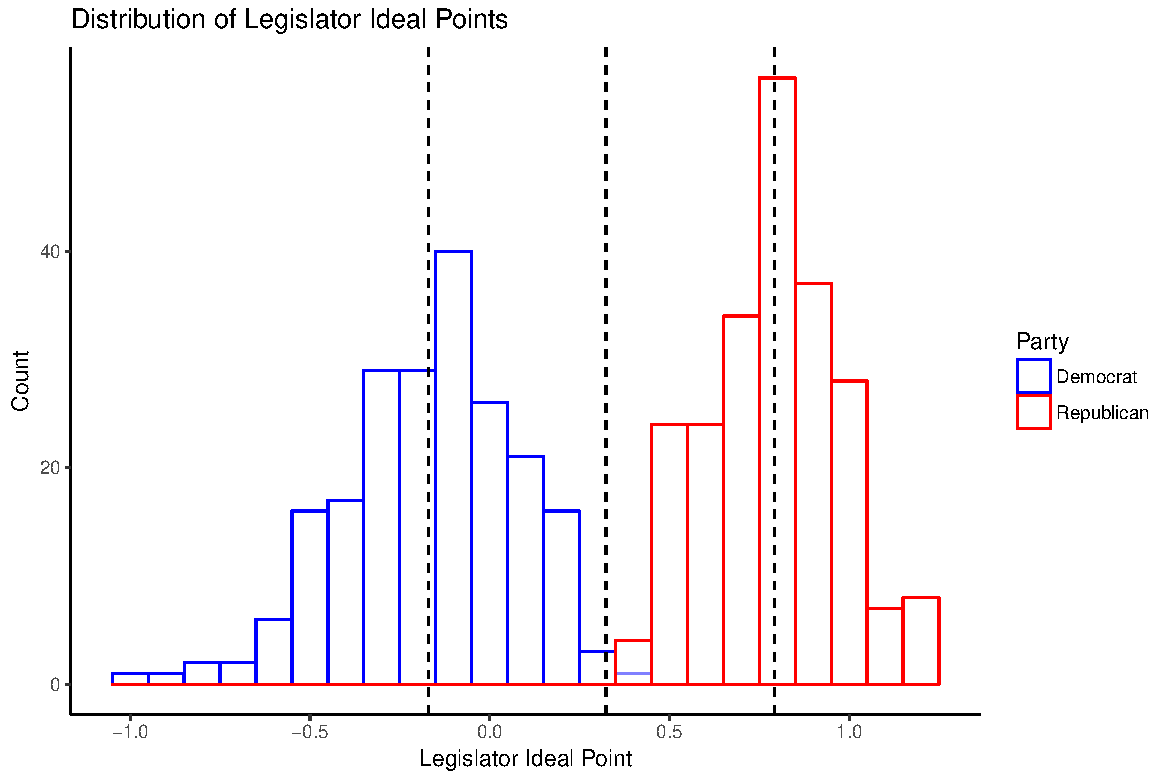
\includegraphics[width=.33\textwidth]{/Users/dsimp/GitHub/Clinton(2006)Rep/drafts/histogram/histogram-1} &
    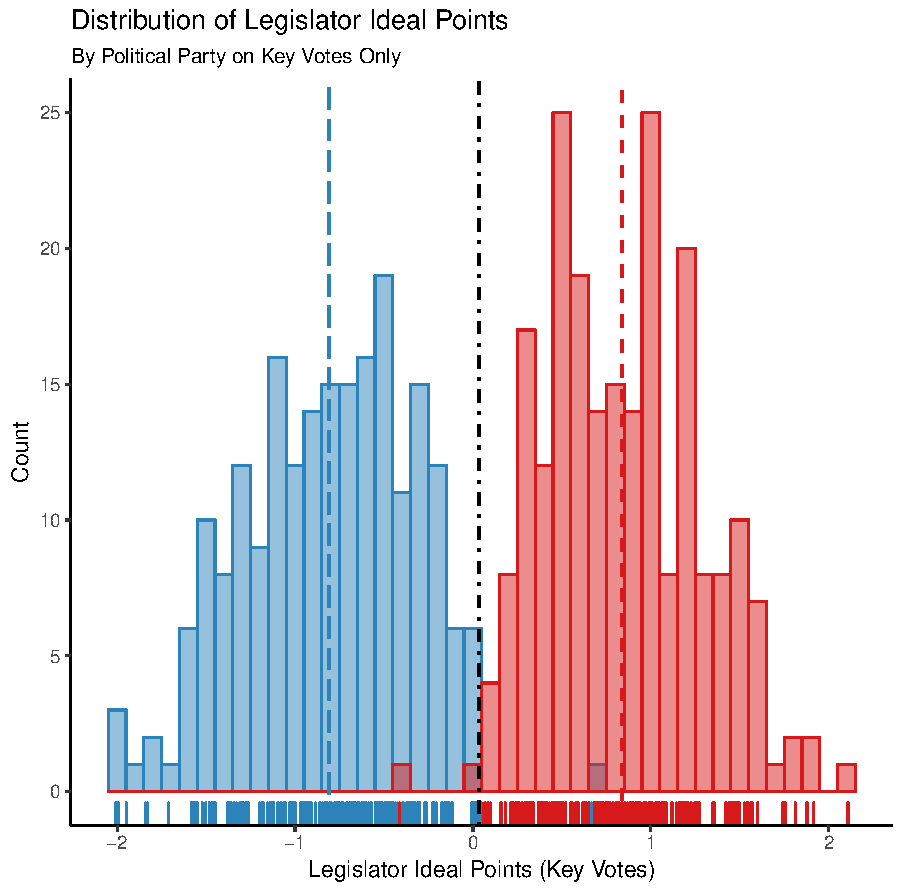
\includegraphics[width=.33\textwidth]{/Users/dsimp/GitHub/Clinton(2006)Rep/drafts/histogram/histogram-2} &
    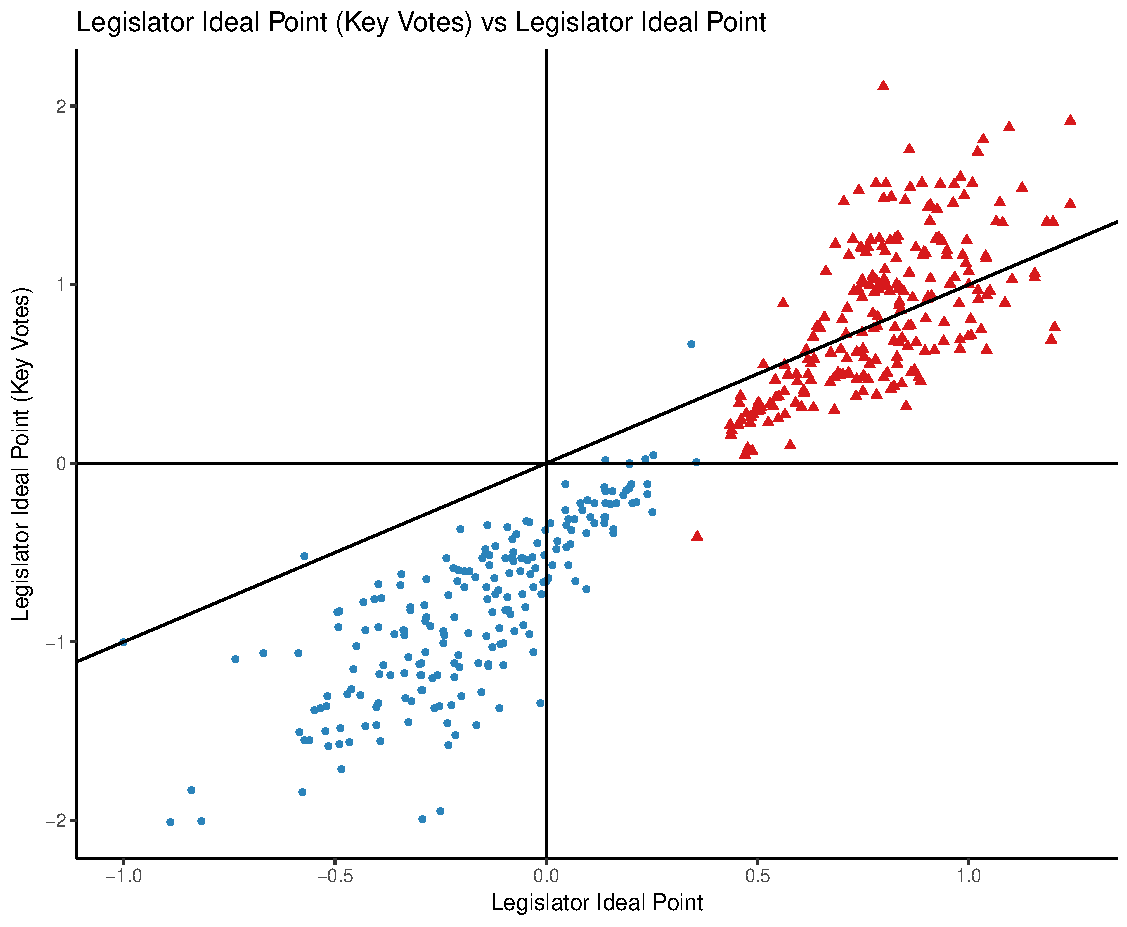
\includegraphics[width=.33\textwidth]{/Users/dsimp/GitHub/Clinton(2006)Rep/drafts/histogram/histo_change} \\
     & &  \\
    \small (D) District Mean Ideology &
    \small (E) Same-Party Mean Ideology &
    \small (F) Non-Same-Party Mean Ideology  \\
	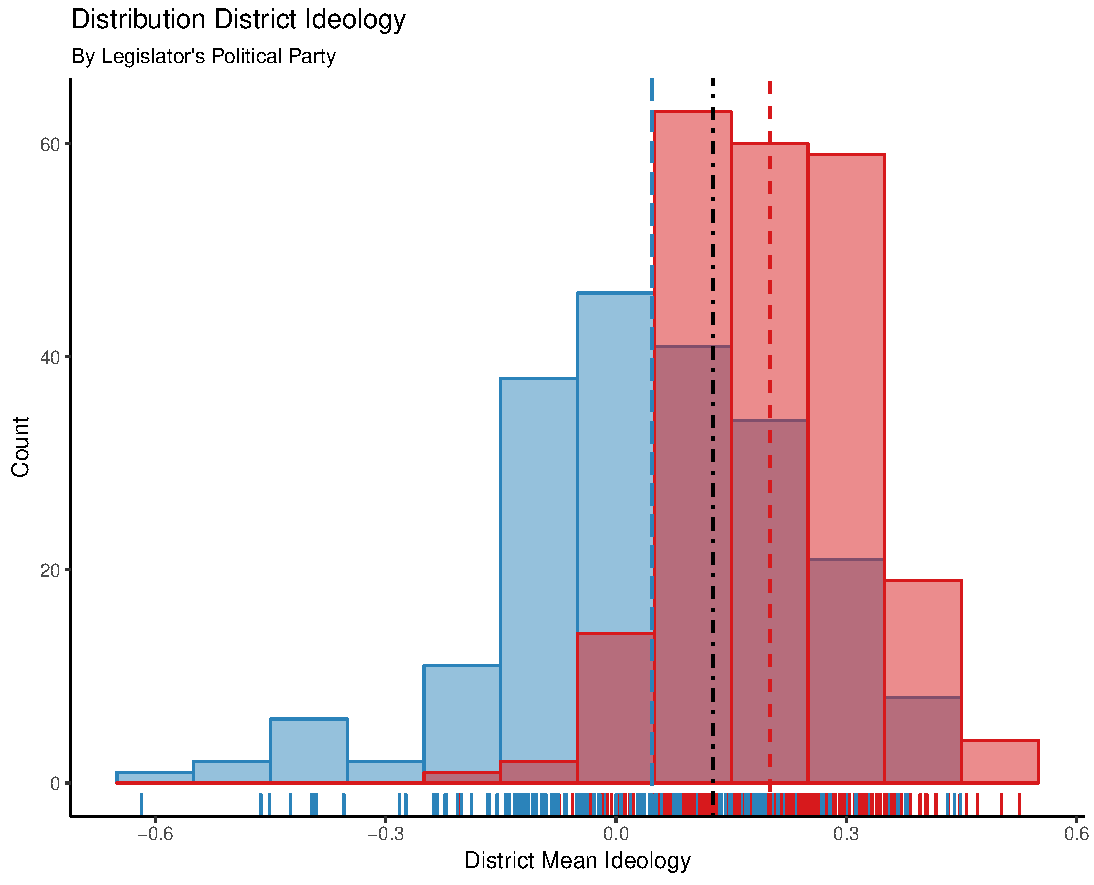
\includegraphics[width=.33\textwidth]{/Users/dsimp/GitHub/Clinton(2006)Rep/drafts/histogram/histogram-3} &
    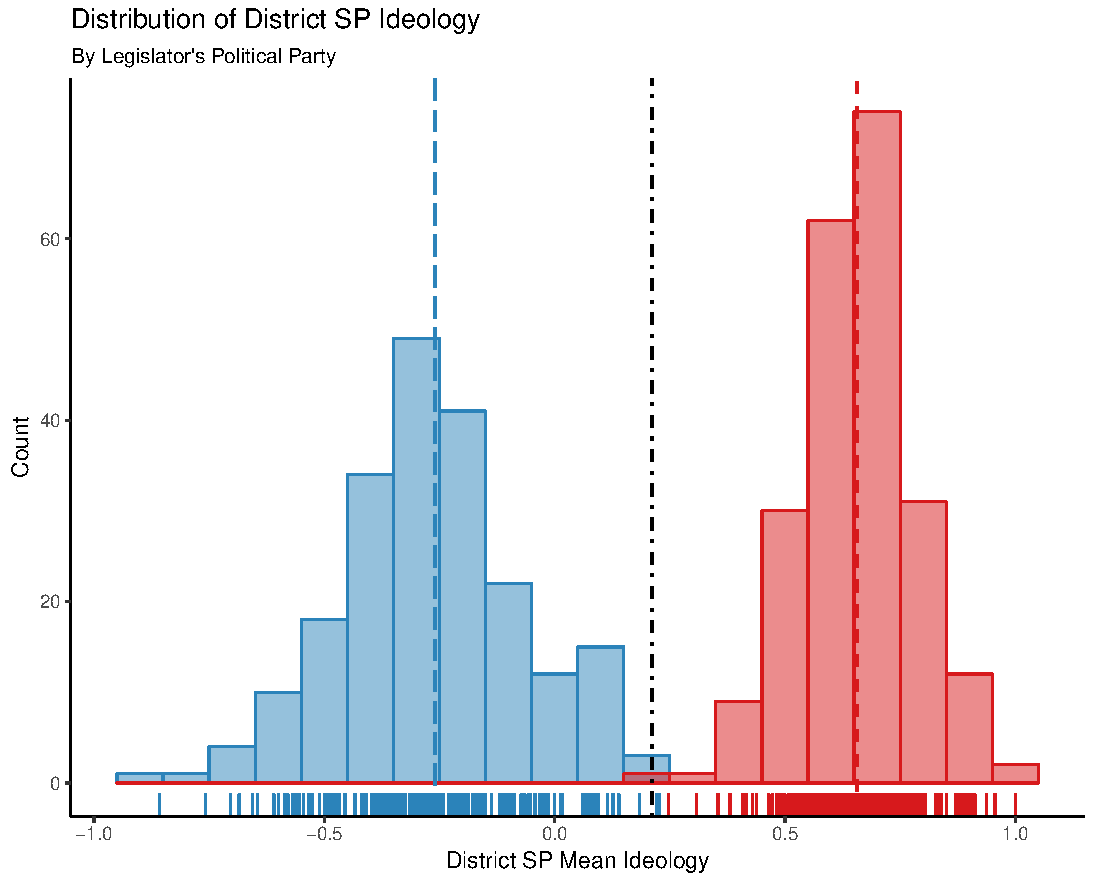
\includegraphics[width=.33\textwidth]{/Users/dsimp/GitHub/Clinton(2006)Rep/drafts/histogram/histogram-4} &
    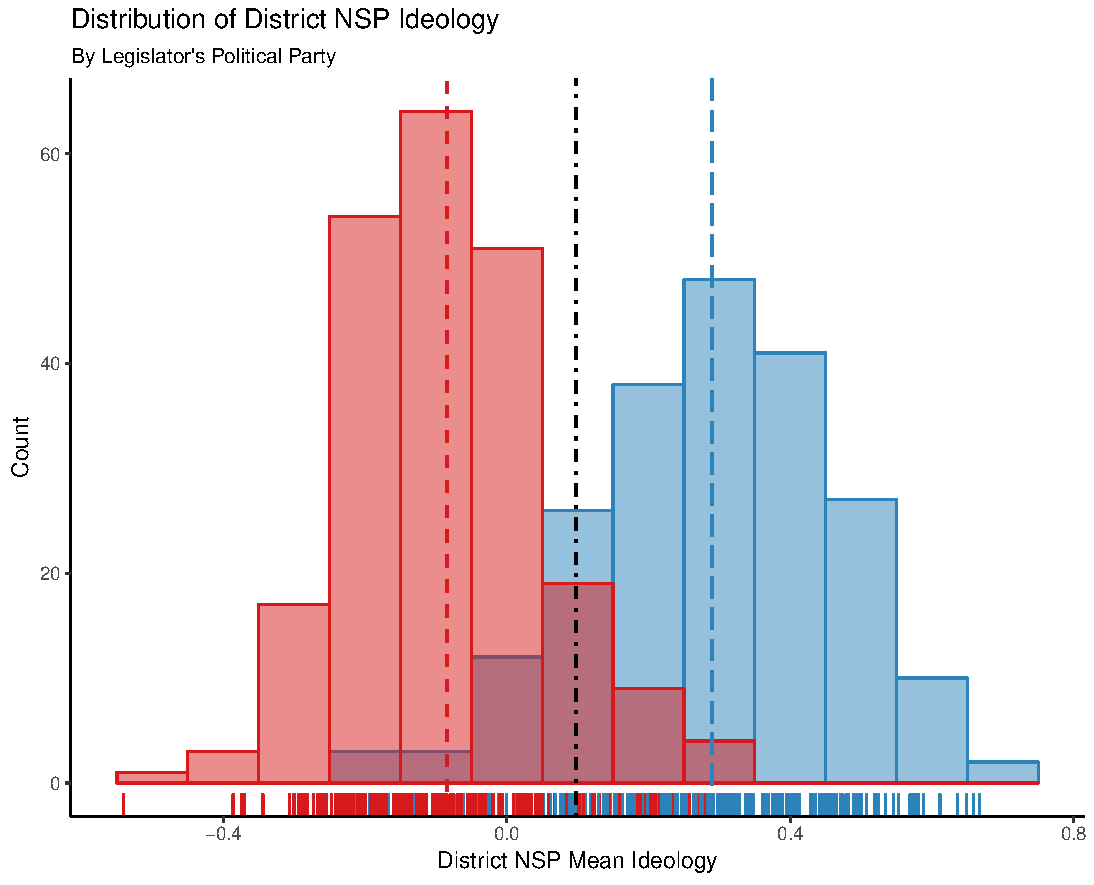
\includegraphics[width=.33\textwidth]{/Users/dsimp/GitHub/Clinton(2006)Rep/drafts/histogram/histogram-5} \\
      & &  \\
    \small (G) Opposite Party Mean Ideology&
    \small (H) Independent Mean Ideology&
    \small (I) Opposite Party vs Independent  \\
    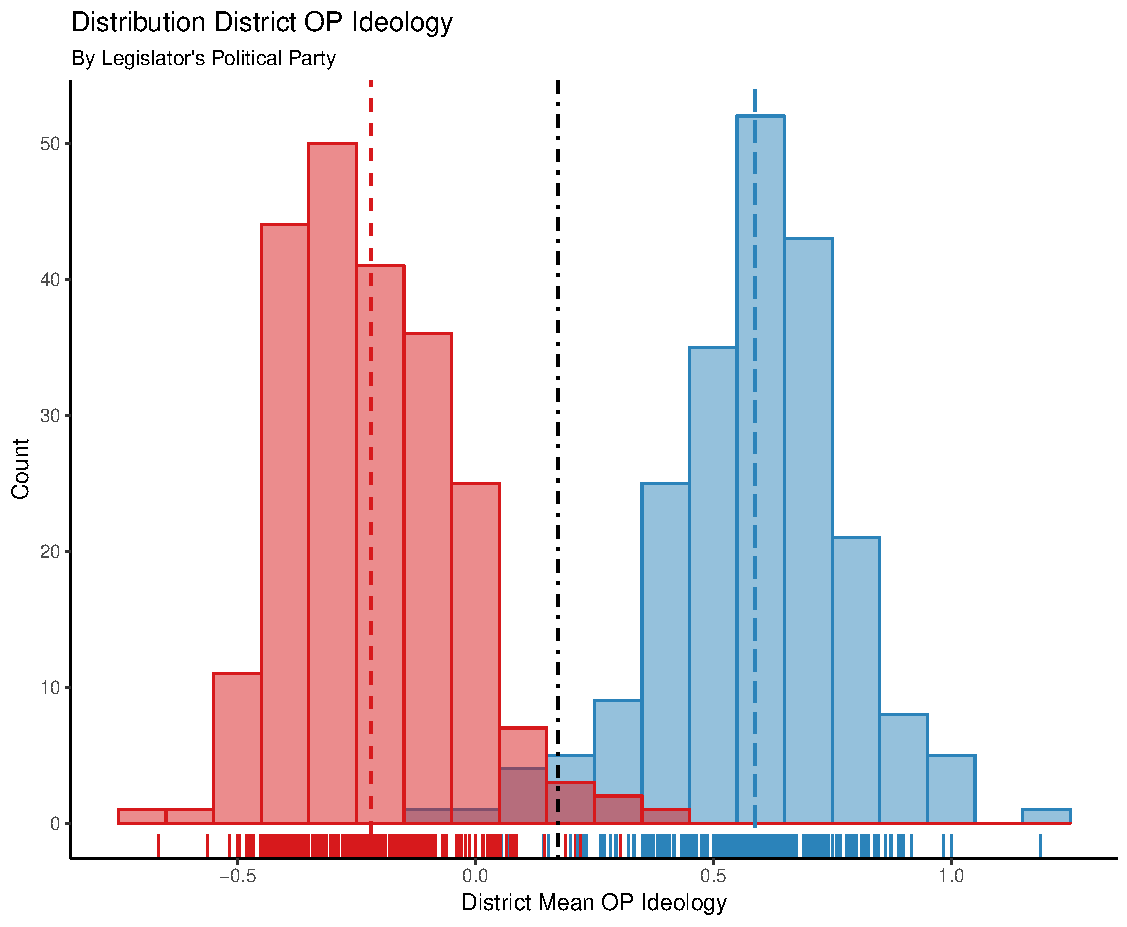
\includegraphics[width=.33\textwidth]{/Users/dsimp/GitHub/Clinton(2006)Rep/drafts/histogram/histogram-6} &
    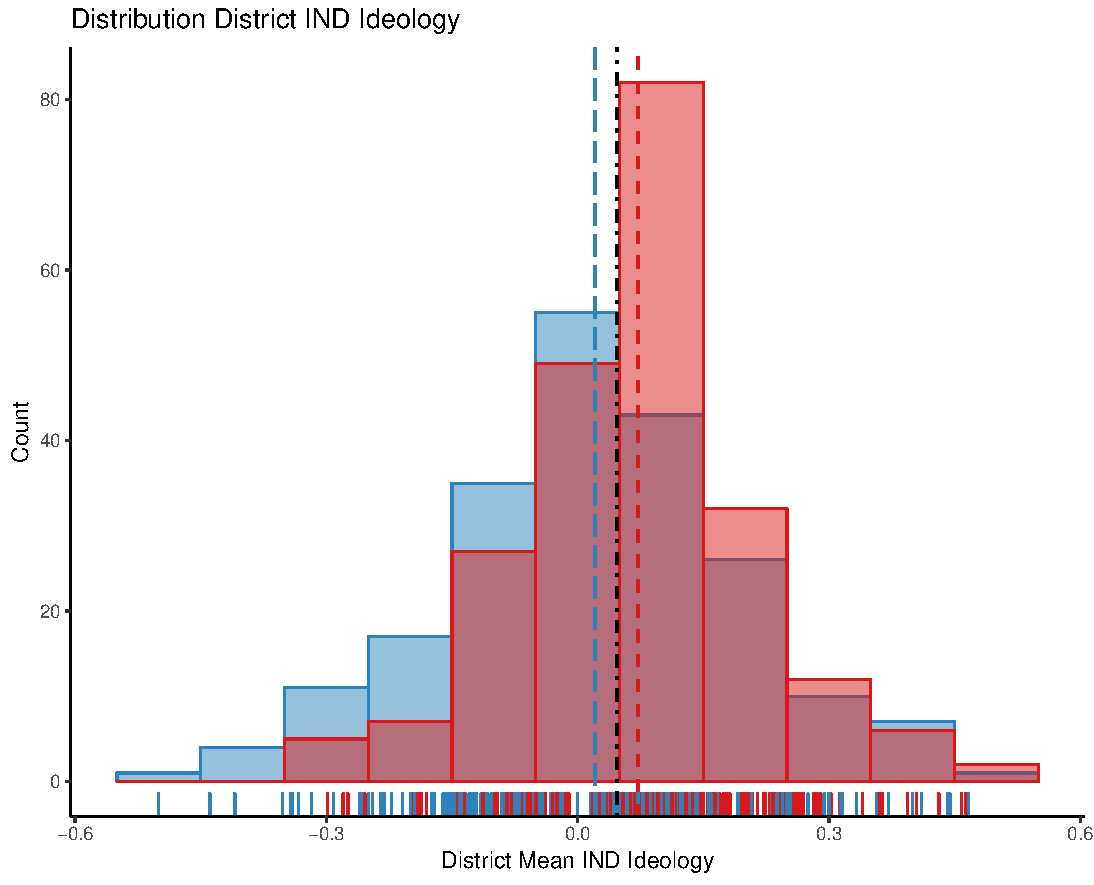
\includegraphics[width=.33\textwidth]{/Users/dsimp/GitHub/Clinton(2006)Rep/drafts/histogram/histogram-7} &
    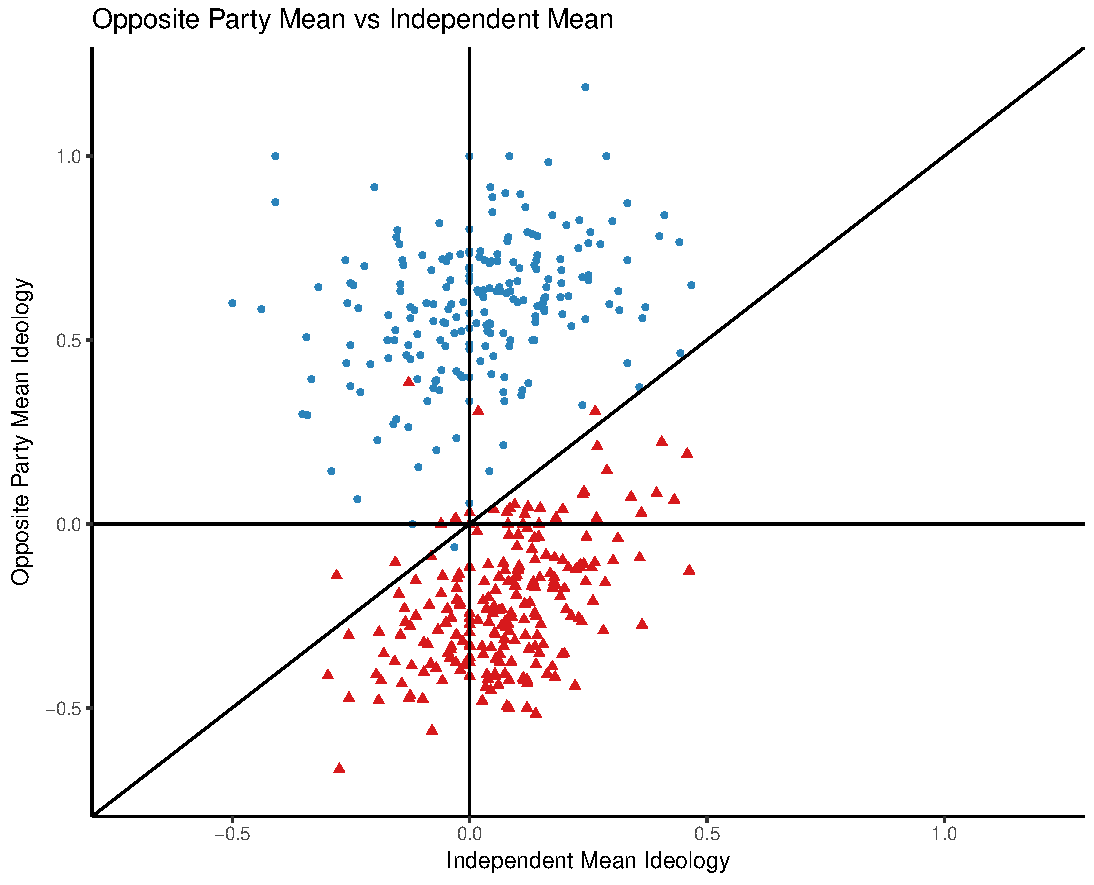
\includegraphics[width=.33\textwidth]{/Users/dsimp/GitHub/Clinton(2006)Rep/drafts/histogram/histo_diff} \\
       & &  \\
  \end{tabular}
    %}   
 \end{centering}\\
  \small \textbf{Note:} The histograms illustrate the distribution of legislator ideal points and sub-district constituency mean ideology grouped by legislator party. For histograms, the short dashed lines are the Republican means, the long dashed line are the Democratic means, and the dotted and dashed line is the chamber mean. Plot (C) shows the change in district district ideal point when key votes are used instead of all votes. Points above (below) the 45-degree line are more conservative (liberal) when key votes are used. Plot (I) compares district independent mean ideology to district opposite party mean ideology. Members with points above (below) the 45-degree line have opposite party constituents more conservative (liberal) than their independent constituents. 
\end{figure} 

The signaled vs revealed phenomenon is similar to but distinct from the delegate paradox described by \cite{Broockman2016} and \cite{Ahler2018}. As stated, the delegate paradox indicates that a vote index can exaggerate the degree of extreme partisanship in a legislative chamber by making moderate legislators appear as extreme ideologues. The paradox is one of the many reasons why \textbf{Lax, Phillips and XXX} use for XYZ analysis. \textbf{Broockman and Ahler} state that the delegate paradox illustrates that an index is more reflective of ideological consistency rather than ideological extremity \textbf{(cite p. N)}. Since the signaled vs revealed phenomenon relies on a index of votes it is important to interpret the index scores as capturing consistency rather than extremity. Similar to \textbf{Ahler and Broockman (2018)'s} findings, the signaled vs. revealed phenomenon suggests vote based ideology indices are sensitive to the set of votes considered. Careful attention is needed when interpreting an index based on variables that can only take a value $i \in {1,0}$.

The signaled vs revealed phenomenon is unique and novel because it suggests that ideological consistency as measured by key votes differs from ideological consistency as measured by all votes in a way that is predictable using existing theory of Congressional law making and legislative bargaining. Index sensitivity is demonstrated by value differences in index values when key votes are used rather than all votes. \textbf{Since all votes in an index are given equal weight, legislators may intentionally or unintentionally use inconsequential votes to shape the ideology of their signaled ideal point. However, key votes may reveal a more accurate reflection of ideological consistency. (Maybe move)}

There are elements of the above findings that fit within what might be expected during an era of split government. Cameron (XXXX)'s analysis of veto bargaining suggests that the president should be able to extract <xx>. As such, there is reason to believe that key votes are \textbf{blah.} As suggested by \textbf{Name (XXXX)}, there is reason to expect the set of all votes includes many votes intended for ideological signaling. Therefore, it is possible Democrats use these votes to signal bipartisan credibility and Republicans to use these votes to signal partisan reliability. In the context of the Cartel Model of Congress, it is expected that the majority of votes that receive a floor vote are \textbf{blah.}


\textbf{(1)} The Cartel Model of Congress indicates that we should expect floor votes in Congress to reflect BLAH. \textbf{(2)} As pointed out by XYZ, we should expect the distribution of votes across all votes to differ from that of Key Votes. If a high share of the total votes are either unimportant or are intended for ideological signaling, then we might expect the few votes of high importance to have a less conservative distribution. In fact, under split government with a Republican held House and a Democratic President we should also expect the average \textbf{Blank to shift toward the left.} Though we might expect both of these to be true, I cannot separate out this effect \textbf{at this time. At the time of writing, I do not have access to the full data set.} \textbf{CLean uP} Furthermore, it would be interesting to see how voting behavior changes in different Congresses and when the Democratic Party has agenda control.

Figure 1 panels (D) through (H) plot histograms for district mean ideology scores and sub-district group mean ideology scores. Unlike legislator ideal points, the district ideology scores are measured using a 5 point ideology scale and are therefore a better reflection of ideological extremity (\textbf{see Data section cite Clinton and A and B.}). Each panel is separated into two groups: districts with Republican legislators and districts with Democratic legislators. Panel (D) shows that districts with Democratic legislators have a mean score that is more liberal than the average district and more liberal than the average district with a Republican legislator. However, Democratic legislators represent districts with mean ideology scores ranging from very liberal to very conservative. Panel (E) shows that same-party constituents are more polarized than the districts as a whole. 

Panels (F) through (H) show that classifying opposite party constituents and independents as a single non-same-party group masks two distinct underlying distributions and makes non-same-party constituents appear less polarized than same-party constituents. Rather, opposite-party constituents (panel G) are nearly as polarized as same-party constituents. \footnote{The left red (right blue) histogram plots the distribution of opposite-party constituents in districts with a Republican (Democratic) legislator.}The two distributions of independent voters reveals that independent voters are much less polarized than their partisan counterparts.\footnote{A Welch's t-test reveals the difference of means between independents in Republican and Democratic districts is statistically significant. However, it is notable that the distributions of independent mean ideologies are both much closer to a mean of zero.} The mean and standard deviations of the ideology scores are given in Appendix Table A2. Table A2 also contains summary statistics for the group shares of each sub-district constituency as a percent of total district constituents. Appendix Figure A1 plots the distribution of sub-district constituent group shares. The average share of same-party constituents in Republican held districts is 0.39, in Democratic held districts it is 0.45. The standard deviation of same-party shares in Democratic districts is nearly twice that of Republican held districts. As such, it is reasonable to expect that independents play a unique role in districts where legislators must compete for both same-party constituents and independents to reach a majority.

Lastly, Panel (I) plots district independent independent ideology against opposite-party ideology. In general, independents in Republican (Democratic) held districts are more conservative (liberal) than the respective opposite-party constituents. The split is evidence using the 45-degree line. Points above (below) the line indicate that independents are more liberal (conservative) than opposite-party constituents.

\subsubsection{Bivariate Regressions}
Figure 2 depicts twelve simple regression plots that explore the relationship between the primary variables of interest. In each panel, districts represented by a Republican (Democrat) are plotted with a red triangle (blue circle). A bivariate trend line is added for overall district level analysis. Trend lines are also included for party specific analysis in districts held by Republican or Democratic legislators. With the exception of panel (I), the slopes of the overall trend lines differ substantially from the slopes of the party specific trend lines. Together the plots illustrate the necessity for analysis that includes differences by party - especially since some overall trend lines suggest a negative relationships among the considered variable pairings. In contrast, each pairing demonstrates a positive relationship when analyzed by party.

Panels (A) through (E) plot legislator ideal points (all votes) against district mean ideology and sub-district constituent group ideology. Panel (A) is particularly interesting because it illustrates that Republican and Democratic legislators with similar district ideologies vote differently. Clinton (2006) states that such a plot indicates that geographic constituency preferences alone cannot explain voting behavior (p. 401). Though this may be true, it is important to interpret the differences in terms of ideological consistency rather than extremity. Additionally, panel (A) illustrates Clinton's observation that Democratic held districts are less homogeneous than Republican held districts. Panel (B) shows that legislator ideal points are consistently more conservative as district ideology becomes more conservative. Similar to Figure 1 panels (F) through (H), Figure 2 panels (C) through (E) show that the relationship between ideal point and non-same party ideology is different than that of ideal points and either independent ideology or opposite party ideology. Across all panels, it is evident that as constituent ideology becomes more conservative so does legislator ideal points.

Though the panel (A) through (E) plots show a relationship between legislator ideological consistency and constituent ideology, it should be expected that legislators respond to both group size and ideology. Appendix Figure 2A depicts the relationship between legislator ideological consistency and group size. The panels clearly illustrate an expected relationship between legislators and their same party constituents. Increased same-party size is associated with increased ideological consistency. Increased non-same-party size has the opposite relationship. Increased non-same-party size is associated with increased (decreased) ideological consistency of non-same-party (same-party) ideology. The opposite-party and independent party plots indicate that opposite party size is the likely the main factor in the observed relationship between non-same-party size and legislator ideal points.

Panels (F) through (I) illustrate that increases in district ideological conservativism is associated with increases in sub-district constituent group conservativism. However, there are still differences by party identification. For example, panel (F) shows that both Republican and Democratic same-party constituent ideology has a positive linear relationship with district ideology. Yet, as a whole Republican same-party constituents are more conservative than Democratic same-party constituents. Similarly, panel (H) shows a positive trend between opposite party ideology and district ideology. Opposite-party constituents with Democratic legislators are more conservative than opposite-party constituents with Republican legislators. In contrast, there seems to be no party effect for Independent voters. In panel (I) average independent ideology is more conservative in more conservative districts; however, there does not seem to be an identifiable difference between independent ideology among districts with similar ideologies but different partisan representatives. This finding is novel for two reasons. First, Table A2 indicates that on average the share of same-party constituencies is less 50\% for districts with legislators of either party. (Though Democratic districts have a larger same-party mean and standard deviation). Second, A2 indicates that independent ideology is less partisan. As such, it should be expected that legislators of each party do have to compete for independent votes. The finding provides additional evidence that classifying independent voters together with opposite party voters may lead to misinterpretation.

Panels (J) through (L) plot sub-constituent ideologies against same party ideologies. \textbf{Add explanation in the next draft.} Plot (L) indicates that Independents in Republican districts are more liberal than self-identified Republicans. Similarly, most Independents in Democratic districts are more conservative than self-identified Democrats. However, independents are not uniformly less polarized than same-party constituents. Observe  that the horizontal $y=0$ line splits both the plotted sets of Republican and Democratic held districts. Regardless of legislator party affiliation, plot (L) indicates that districts with similar same-party ideologies may have on average either conservative leaning or liberal leaning independents. \footnote{In next draft add plot of independents vs opposite party constituents in the appendix.} \footnote{In next draft write the hypothesis associated with this paper and the interpretation limits of these hypothesis.}

This next section establishes the necessity for including all constitutive terms and provided some evidence to contradict responsiveness puzzle and to suggest a need to separate non-same-party into independent and opposite party tor analysis of three rather than 2 sub-district constituent groups. In section 5.2, the analysis is expanded to consider three groups. In section 5.3, the analysis looks at the behavior of legislators by party. I section 5.4, the analysis considers explores the signaled vs revealed responsiveness phenomenon in greater detail.

\newpage
\begin{figure}[!htbp]
\caption{Legislator Ideal Points and District Ideology Means}
\begin{centering}
%\centering
%\fbox{
  \begin{tabular}{@{}ccc@{}}
	% & & \\  	
  	\small (A) Ideal Point &
    \small (B) Ideal Point &
    \small (C) Ideal Point  \\
    \small vs District Ideology & 
    \small vs Same-Party Ideology &
    \small vs Non-Same-Party Ideology \\
    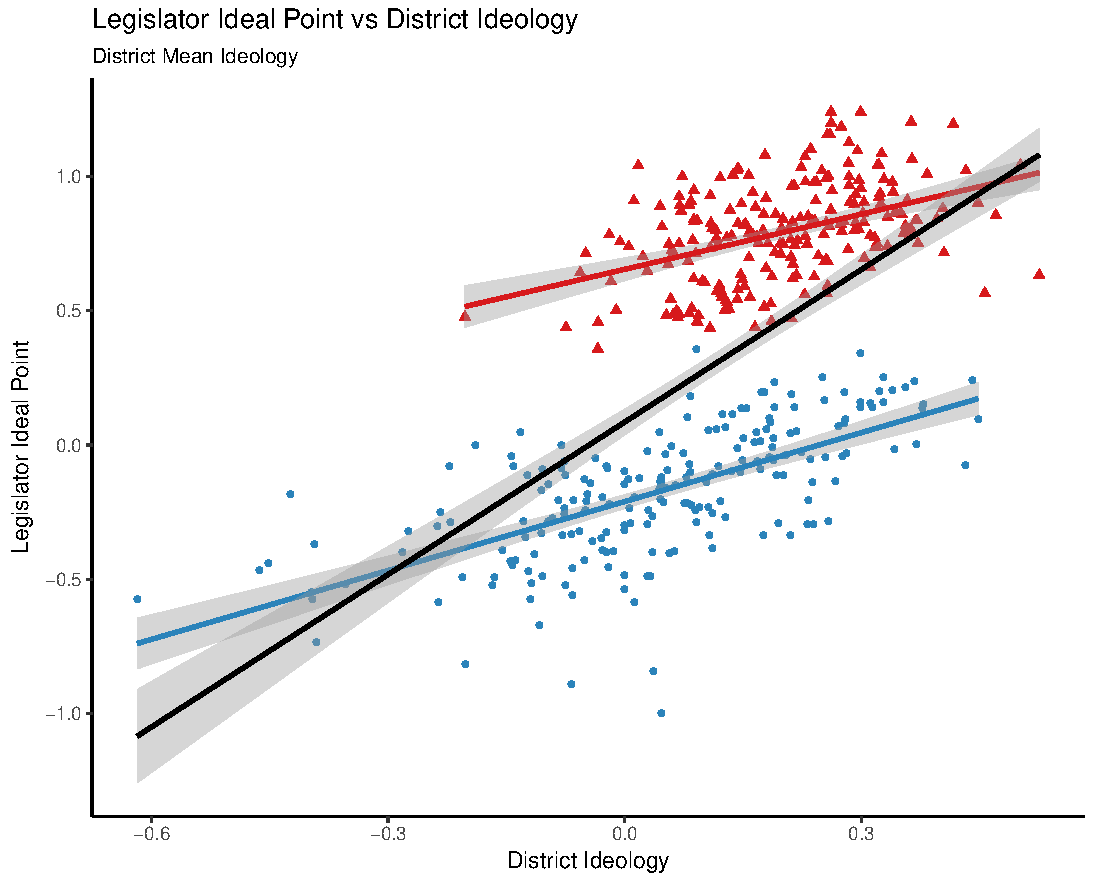
\includegraphics[width=.30\textwidth]{/Users/dsimp/GitHub/Clinton(2006)Rep/drafts/plots/plot1-1.pdf} &
    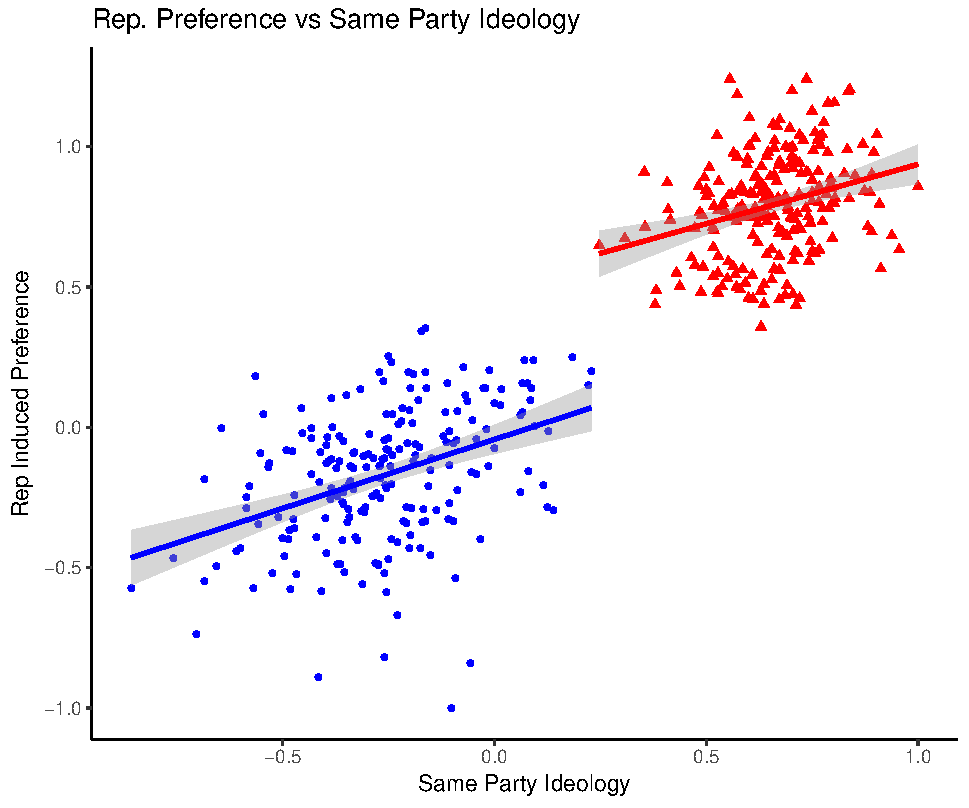
\includegraphics[width=.30\textwidth]{/Users/dsimp/GitHub/Clinton(2006)Rep/drafts/plots/plot1-2.pdf} &
    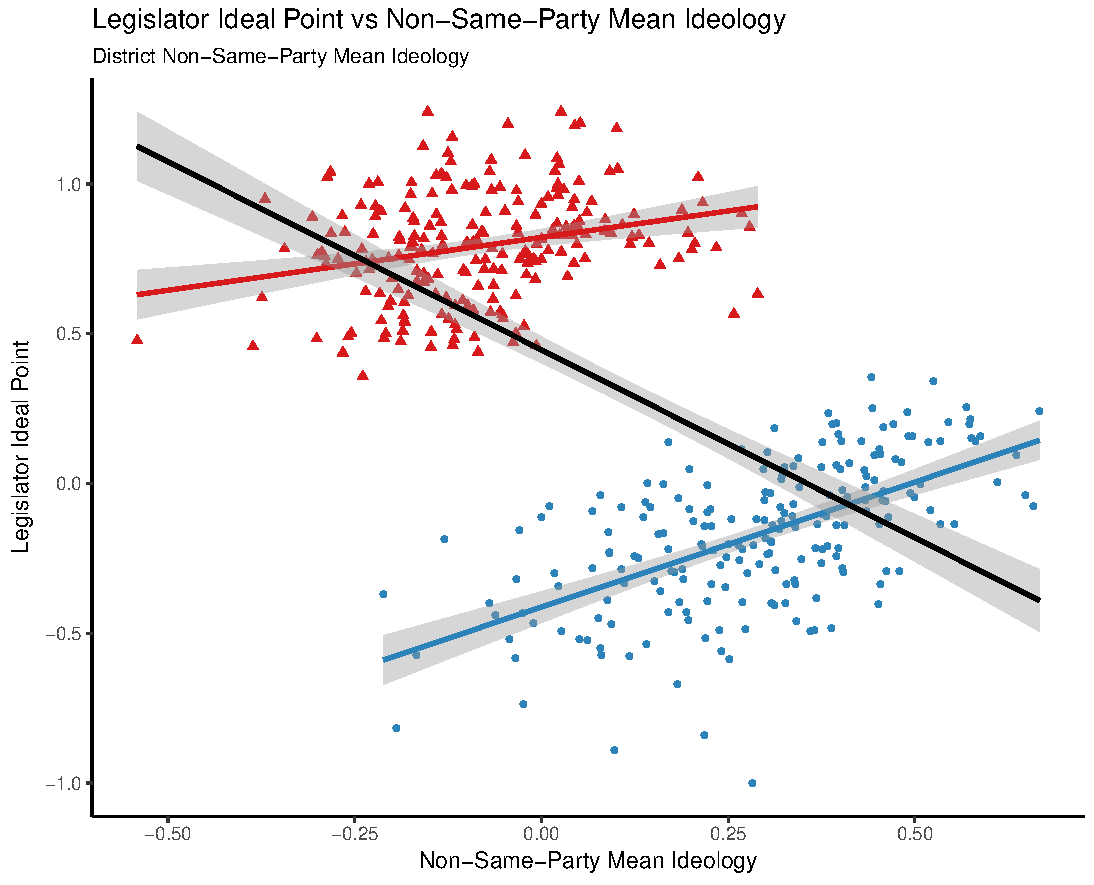
\includegraphics[width=.30\textwidth]{/Users/dsimp/GitHub/Clinton(2006)Rep/drafts/plots/plot1-3.pdf} \\
    % & & \\
    \small (D) Ideal Point & 
    \small (E) Ideal Point & 
    \small (F) Same-Party Ideology  \\
    \small vs Opposite Party Ideology  & 
    \small vs Independent Ideology  & 
    \small vs District Ideology \\
    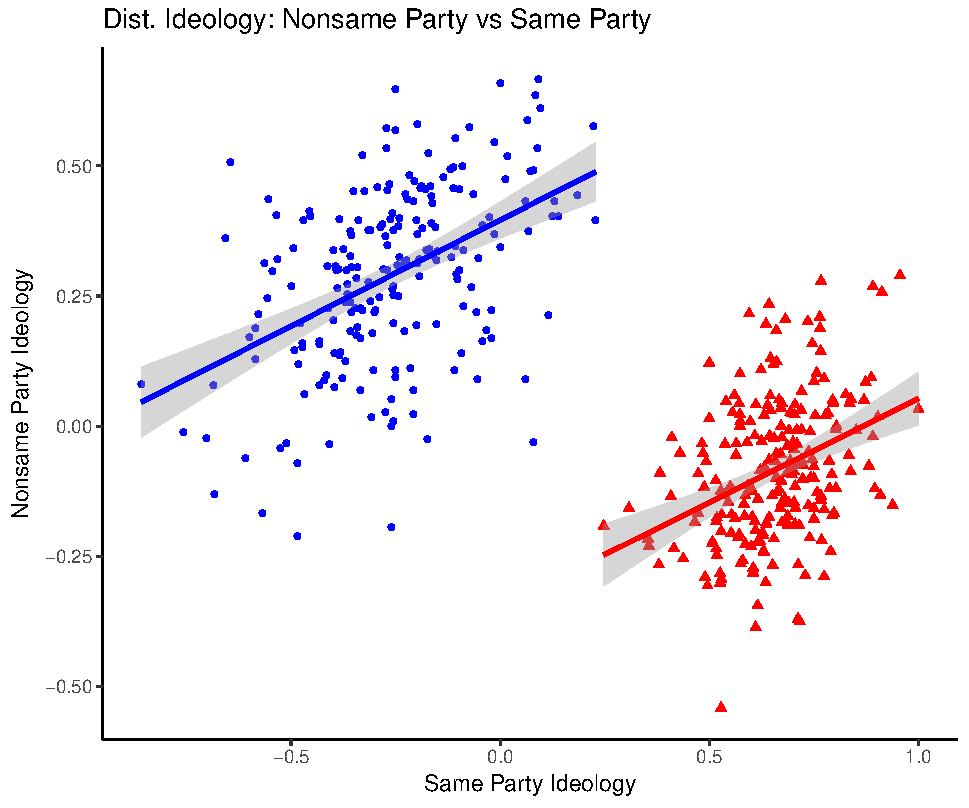
\includegraphics[width=.30\textwidth]{/Users/dsimp/GitHub/Clinton(2006)Rep/drafts/plots/plot1-4.pdf} &
    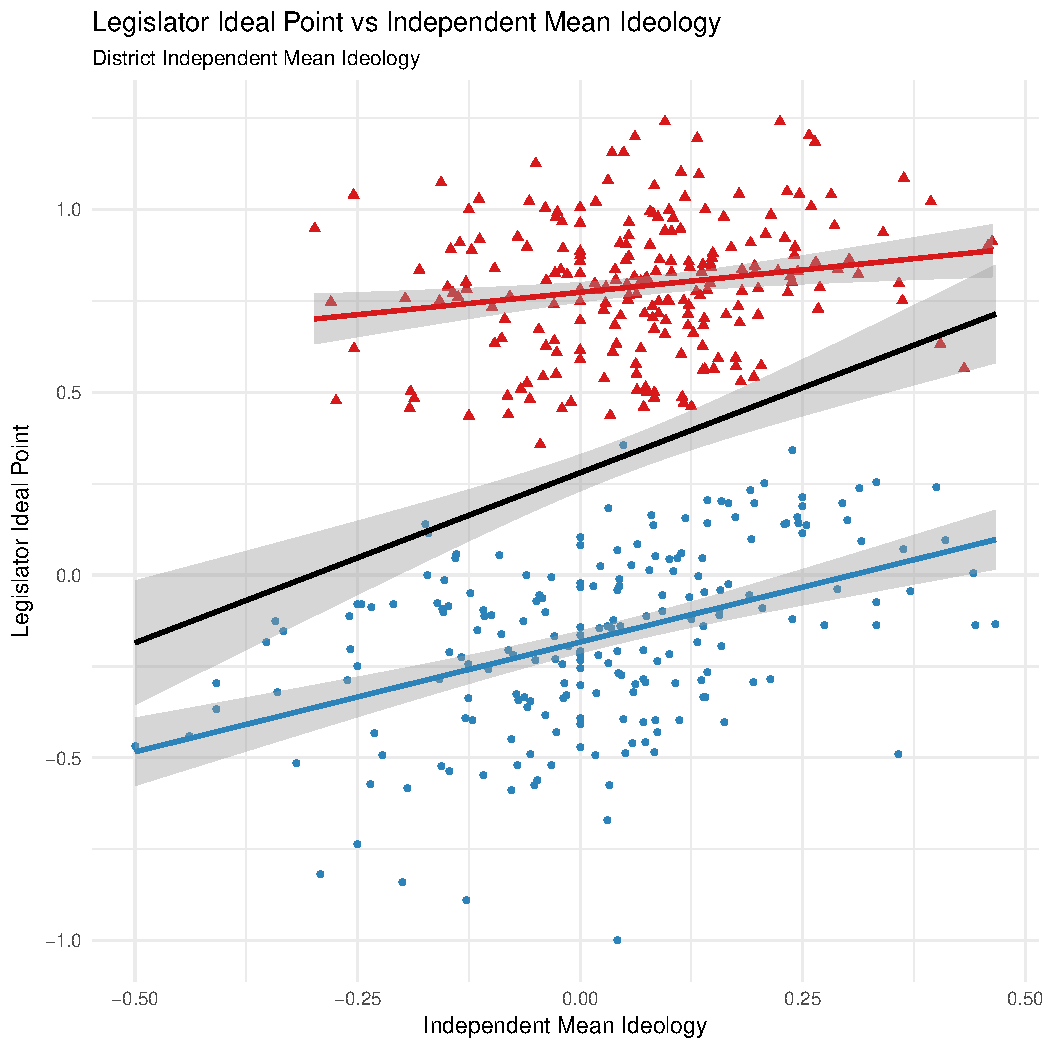
\includegraphics[width=.30\textwidth]{/Users/dsimp/GitHub/Clinton(2006)Rep/drafts/plots/plot1-5.pdf} &
    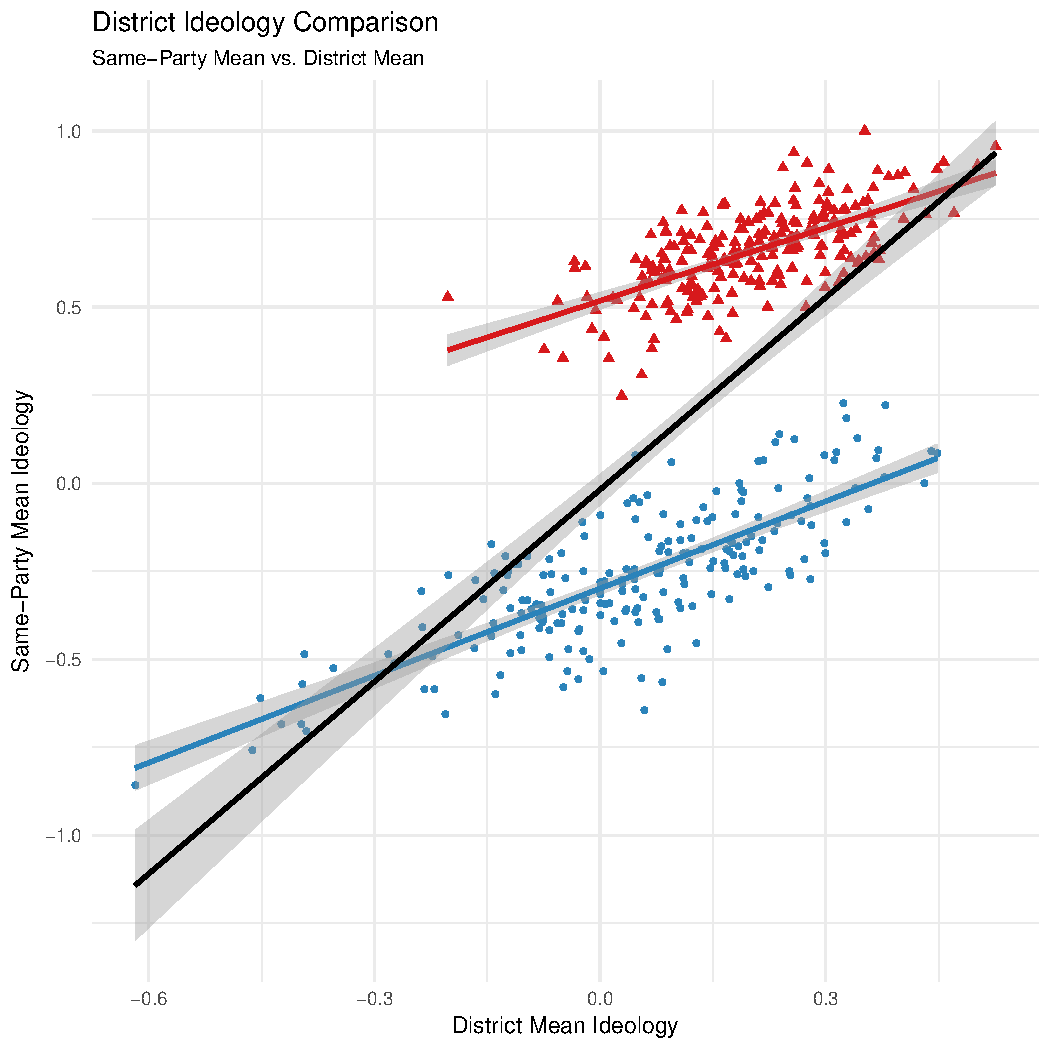
\includegraphics[width=.30\textwidth]{/Users/dsimp/GitHub/Clinton(2006)Rep/drafts/plots/plot1-6.pdf} \\
    % &  &\\
    \small (G) Non-Same-Party Ideology & 
    \small (H) Opposite Party Ideology & 
    \small (I) Independent Ideology  \\
    \small vs District Ideology  & 
    \small vs District Ideology  & 
    \small vs District Ideology \\
    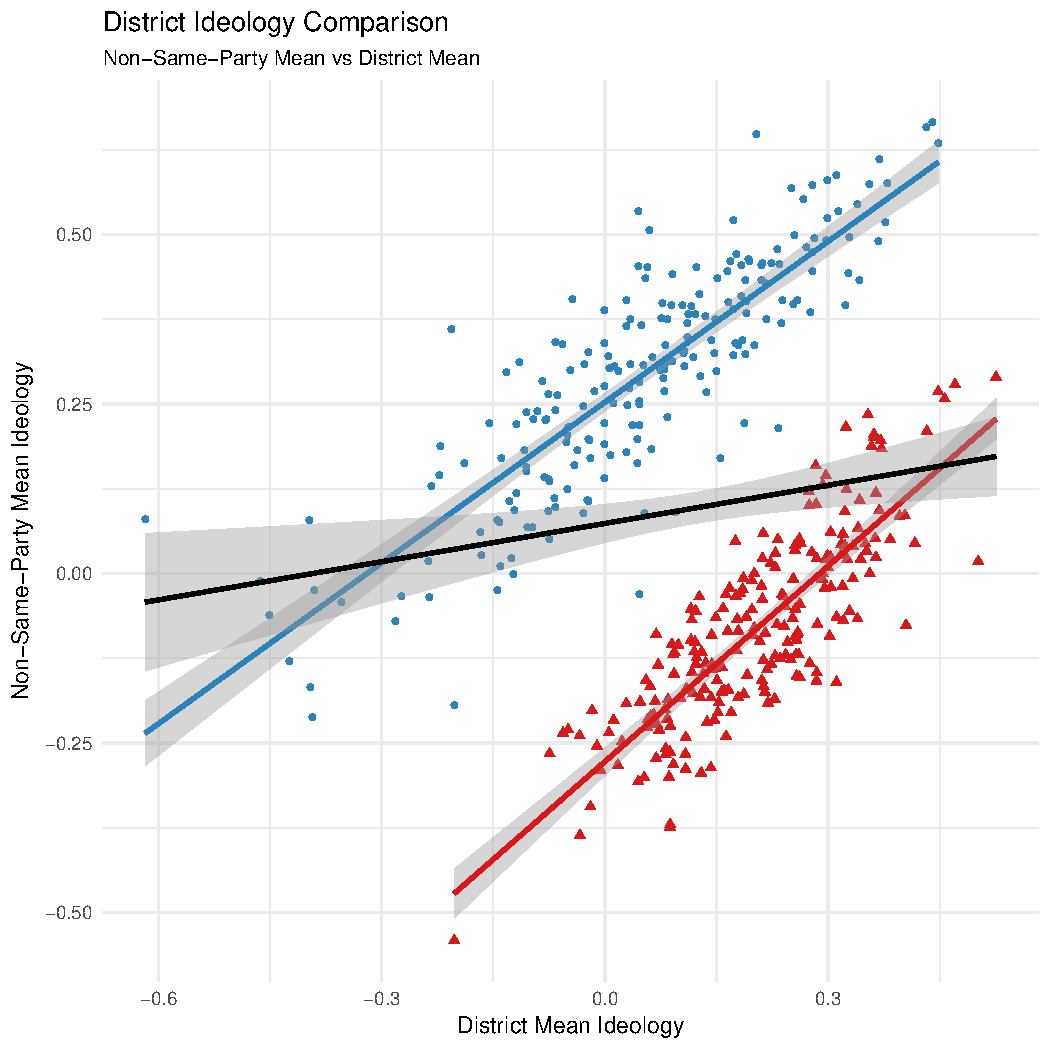
\includegraphics[width=.30\textwidth]{/Users/dsimp/GitHub/Clinton(2006)Rep/drafts/plots/plot1-7.pdf} &
    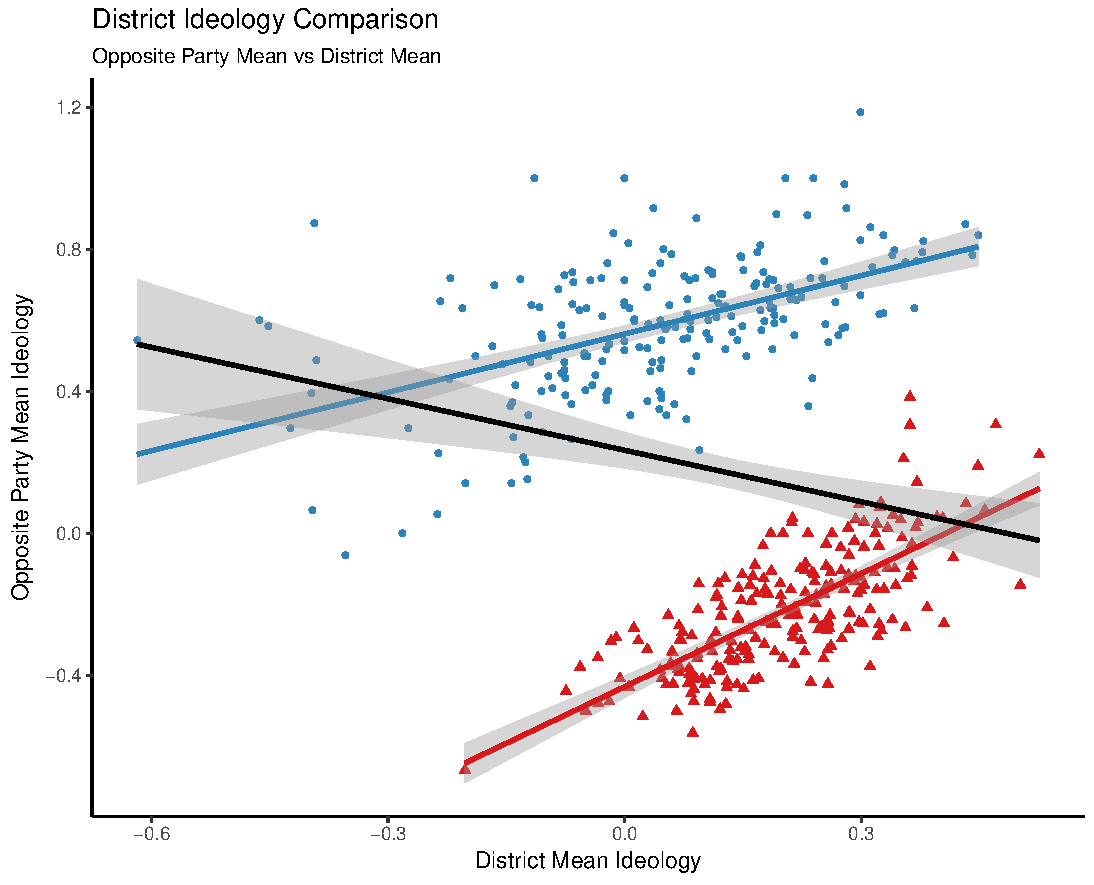
\includegraphics[width=.30\textwidth]{/Users/dsimp/GitHub/Clinton(2006)Rep/drafts/plots/plot1-8.pdf} &
    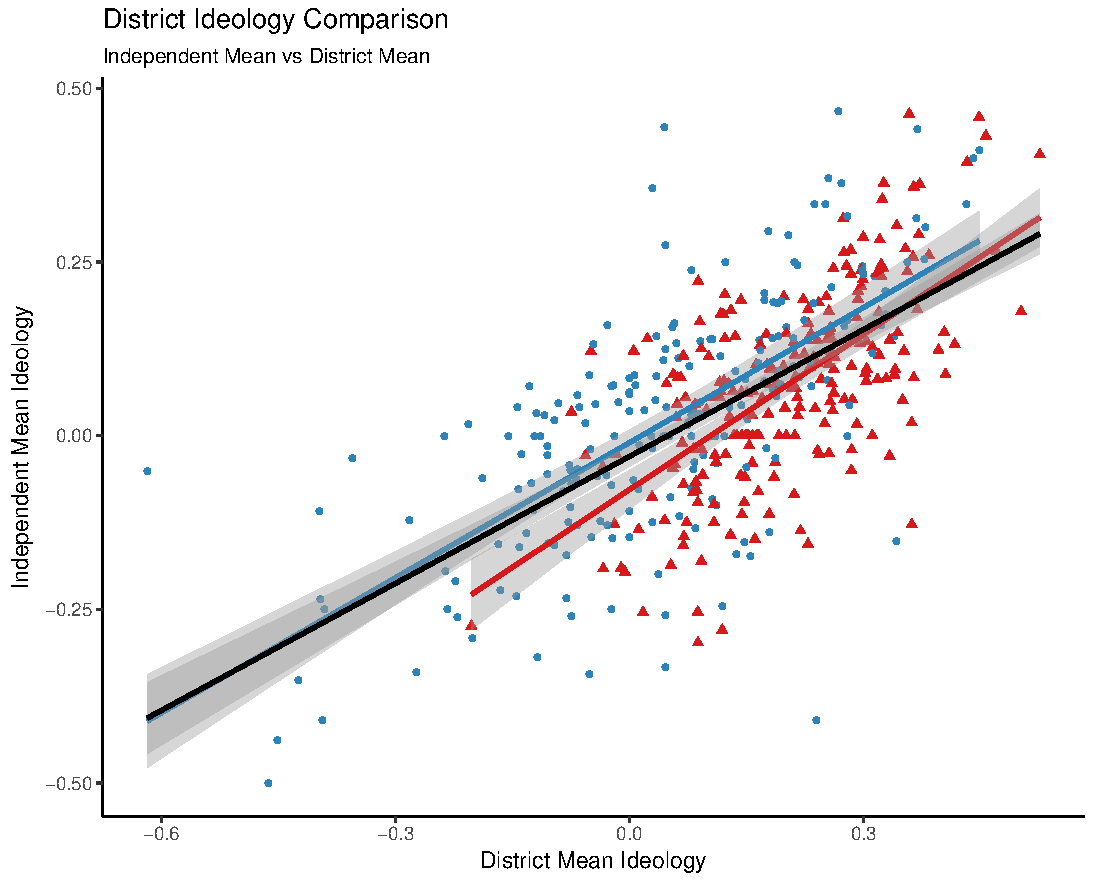
\includegraphics[width=.30\textwidth]{/Users/dsimp/GitHub/Clinton(2006)Rep/drafts/plots/plot1-9.pdf} \\
    % &  &\\
    \small (J) Non-Same-Party Ideology & 
    \small (K) Opposite Party Ideology & 
    \small (L) Independent Ideology  \\
    \small vs Same-Party Ideology  & 
    \small vs Same-Party Ideology  & 
    \small vs Same-Party Ideology \\
    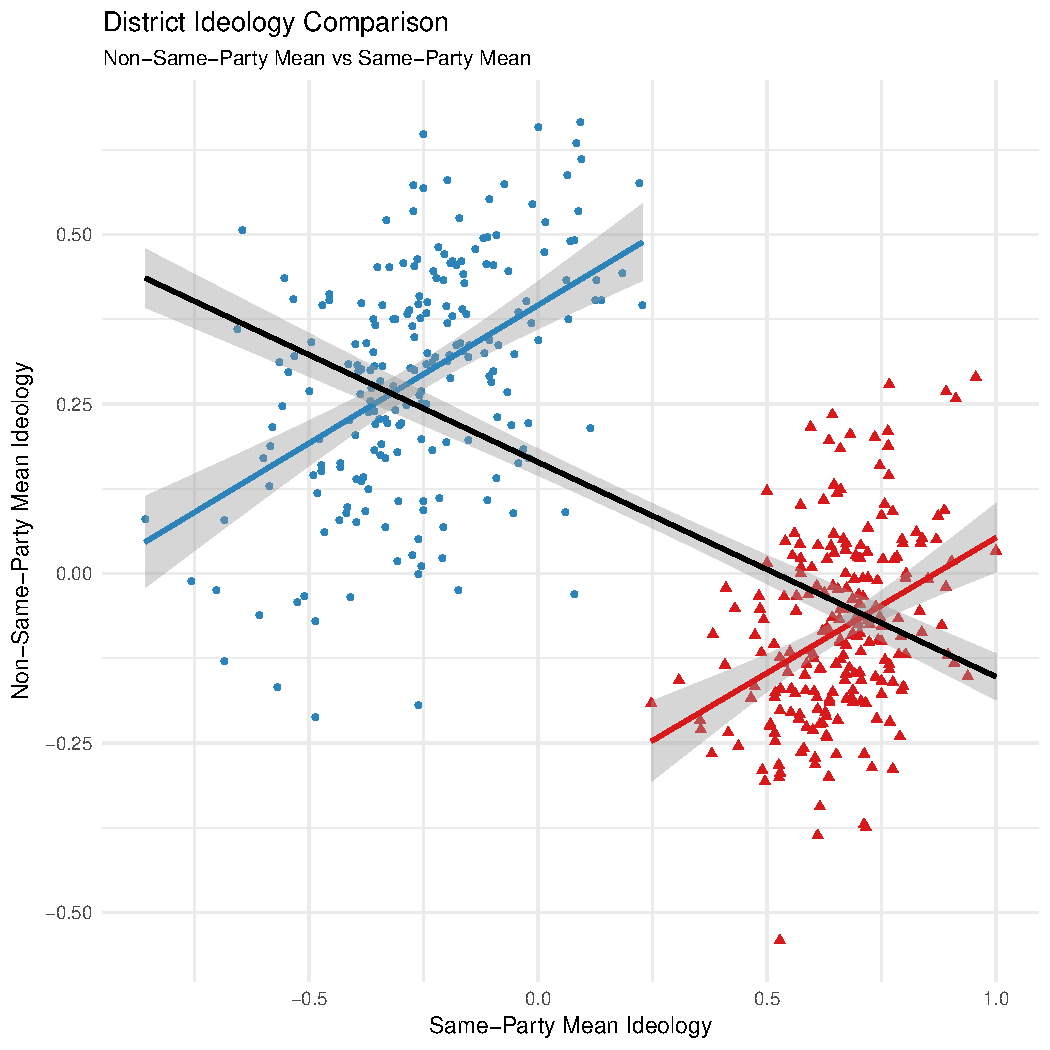
\includegraphics[width=.30\textwidth]{/Users/dsimp/GitHub/Clinton(2006)Rep/drafts/plots/plot1-10.pdf} &
    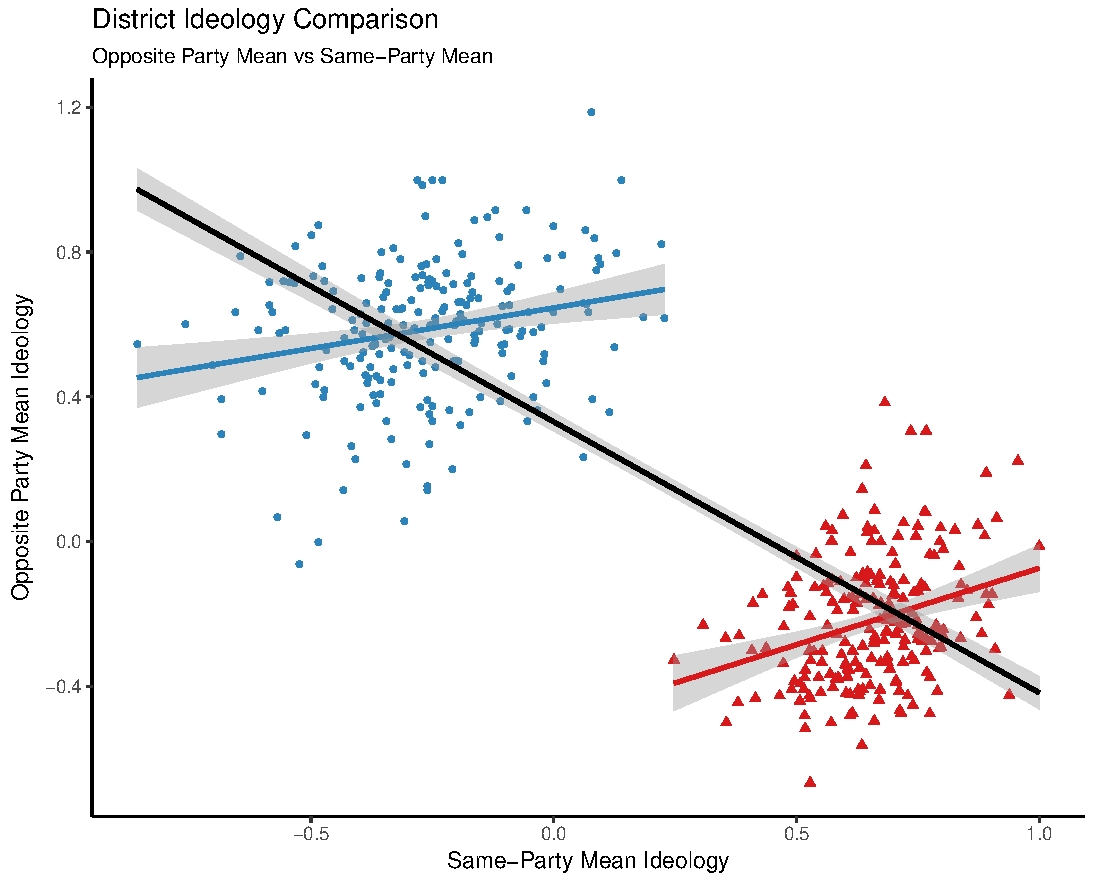
\includegraphics[width=.30\textwidth]{/Users/dsimp/GitHub/Clinton(2006)Rep/drafts/plots/plot1-11.pdf} &
    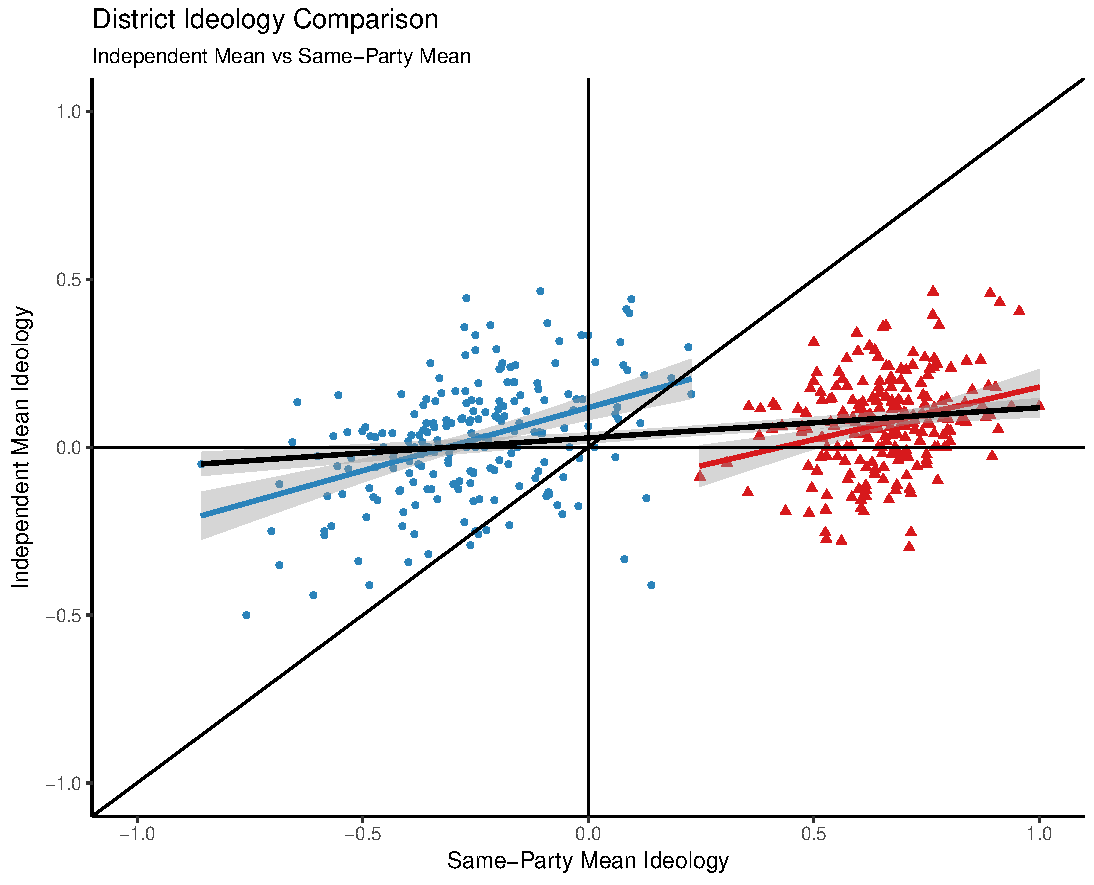
\includegraphics[width=.30\textwidth]{/Users/dsimp/GitHub/Clinton(2006)Rep/drafts/plots/plot1-12.pdf} \\
  \end{tabular}
    %}   
 \end{centering}
 \small \textbf{Note:} Districts represented by Republicans (Democrats) are plotted with triangles (circles). A bivariate trend line is plotted for overall comparison and party trend lines are plotted for comparison within districts.
\end{figure} 
\newpage

\section{Initial Findings} 
The initial findings are split into 4 sections. Section 5.1 illustrates the problem with failing to include constitutive terms in models with variable interactions. It provides unbiased model analysis of legislator responsiveness to two sub-district groups and discusses the implications of the unbiased models. Section 5.2 considers legislator responsiveness to three sub-district groups and argues that lumping independents with opposite-party constituents may conceal underlying unique responsiveness relationships. Section 5.3 uses within party analysis to provide convincing evidence that contradicts the responsiveness puzzle. Section 5.4 provides evidence that suggests that legislator responsiveness to sub-district groups is conditional on the policy significance of considered votes.

\subsection{Interaction Terms}
The main empirical issue in \cite{Clinton2006} is that each model with interaction terms omits the constitutive terms necessary for determining the relationship between sub-district ideology and legislator ideal point. \cite{Brambor2006} demonstrate that there is almost never a valid reason to omit constitutive variables when a model includes interaction terms. Observe the below equation model (1) which appears in Clinton's Table 1 (p. 403). The model regresses legislator (all votes) ideal points ($y_i$) on weighted sub-district level average ideology scores.

\begin{equation}
y_i  = \beta_0 + \beta_1 w_{SP_i} \bar{z}_{SP_i} + \beta_2 w_{NSP_i} \bar{z}_{NSP_i} + \gamma I_{GOP} + \varepsilon_i
\end{equation}
The terms $w_{SP_i}$ and $w_{NSP_i}$ respectively weight same-party average ideology ($\bar{z}_{SP_i}$) and non-same-party average ideology ($\bar{z}_{NSP_i}$) by the share of group members sampled in each district. As such, the weights in equation model (1) are defined as $w_{SP_i} = \frac{n_i^{SP}}{n_i}$ and $w_{NSP_i} =  \frac{n_i^{SP}}{n_i}$. The term $I_{GOP}$ is a party indicator variable. The above specification yields biased coefficient values and underestimated coefficient standard errors. The unbiased specification of model (1) should include $w_{SP_i}$, $w_{NSP_i}$, $\bar{z}_{SP_i}$, $\bar{z}_{SP_i}$ each as individual independent variables in addition to their respective interaction terms. As such, the unbiased specification is given in the below equation model (2).
\begin{equation}
\begin{array}{ccc}
y_i & = & \alpha_0 + \alpha_1 w_{SP_i} \bar{z}_{SP_i} + \alpha_2 w_{NSP_i} \bar{z}_{NSP_i} + \alpha_3 \bar{z}_{SP_i}~~~~~~~~~\\ 
& & ~~+ \alpha_4 \bar{z}_{NSP_i} + \alpha_5 w_{SP_i} + \alpha_6 w_{NSP_i} + \lambda I_{GOP} + \epsilon_i
\end{array}
\end{equation}
Model (1) implies that one can estimate the unconditional marginal effect of weighted group ideology (i.e. $\beta_1$ for the single term $\frac{n_i^{SP}}{n_i} \bar{z}_{SP_i}$) and that neither the weights nor sub-district group ideologies have an independent effect on legislator ideal point. Empirically, model (1) implicitly assumes that $\alpha_3$, $\alpha_4$, $\alpha_5$, and $\alpha_6$ from model (2) are all zero. Intuitively, one should expect group size $w_{j\in \{SP,NSP\}_i}$ and group ideology $\bar{z}_{j\in \{SP,NSP\}_i}$ to each individually influence legislator behavior. One should also expect the impact of group share (group ideology) to change as group ideology (share) changes.

Empirically, the marginal effect of group share (group ideology) is given by the derivative of legislator ideal point with respect to share (ideology). For example in equation (2), the relationship between legislator ideal point and same-party ideology is: 
$$\frac{\partial y_i}{\partial \bar{z}_{SP_i}}= \alpha_1 w_{SP_i} + \alpha_3$$
The coefficient $\alpha_3$ captures the portion of the slope $\frac{\partial y}{\partial \bar{z}_{SP_i}}$ (the relationship between ideal point and same-party ideology) that is constant across all districts regardless of the district share of same-party constituents. The term $\alpha_1 w_{SP_i}$ captures how the slope $\frac{\partial y}{\partial \bar{z}_{SP_i}}$ changes as the district share of same-party constituents increases. Therefore model (2) is underspecified and the estimates of $\beta_1$ and $\beta_2$ will be biased. %For example, the coefficient $\beta_1$ on weighted same-party ideology in equation (1) is capturing $\alpha_1$, $\alpha_3$ and $\alpha_5$ from equation (4). % Uncomment to reinsert

Additionally, it is important to note that the use of interaction terms implies that a second calculation is necessary to determine the standard errors for the marginal effects of group share or group ideology. One cannot rely on the usually reported coefficient values and standard errors to determine statistical significance of a variable that is included in an interaction term. Rather, it is necessary to directly calculate the variance term. For example, consider the marginal effect of same-party ideology. The variance is given as:  $var(\frac{\partial y}{\partial \bar{z}_{SP_i}})$. That is $var(\frac{\partial y}{\partial \bar{z}_{SP_i}}) = var(\alpha_1 w_{SP_i} + \alpha_4)$. Therefore, the standard error term for $\frac{\partial y}{\partial \bar{z}_{SP_i}}$ is given by:
$$\hat{\sigma}_{\partial y_i / \partial \bar{z}_{SP_i}} = \sqrt{w_{SP}^2var(\hat{\alpha}_1)+var(\hat{\alpha}_3)+2w_{SP}cov(\hat{\alpha}_1\hat{\alpha}_3)}$$

\textbf{Results:} Table 2 provides the regression results for models 1 and 2. Model 1 is the identical replication of Clinton (2006)'s model without the constitutive terms. Model 2 is the unbiased model specification with each of the interaction terms. Under this specification, one cannot estimate the marginal effect of Percent Non-Same Party because percent Same-Party and Percent Non-Same Party are perfectly multicolinear by construction. Therefore, there is no Percent Non-Same-Party coefficient estimate.  Model 3 omits the constant term to allow for estimation of the marginal effect of Percent Non-Same Party. \footnote{Need to italicize the variable terms in the next draft.}

Comparison of the regression results from model 1 and model 3 show that the coefficient estimates for the model 1 interaction terms are downwardly biased with smaller standard errors. In the unbiased model 3 specification, the coefficients on three of the four constitutive terms are significant. However, the point estimates should not be used for simple interpretation. The coefficient on same-party ideology and the plots in Figure 3 perfectly illustrate this point.  Figure 3 plots the marginal effects of group ideology and group share on legislator ideal point. Each plot also contains a rug and distribution plot of group ideology or share to help visualize how  the marginal effect of group share (group ideology) changes at different ideology (share) levels.

\textit{Same-Party Share:} The coefficient point estimate on same-party share indicates that same-party share  does not have a significant effect on legislator ideological consistency. However, panel (A) shows that the magnitude of legislator responsiveness to same-party share increases with constituent ideological extremity. The effect of same-party share on legislator ideological consistency is more positive/conservative (negative/liberal) as same-party ideology becomes more conservative (liberal). Therefore, the results suggest that increases in same-party ideological extremity are associated with increases in the ideological consistency signaled by legislator votes. 

\textit{Same-Party Ideology:} Panel (B) shows that the marginal effect of same-party ideology becomes more positive/conservative with increases in same-party share. Therefore, as the percent same-party increases, the associated positive effect on the conservative ideological consistency of legislators also increases. This implies that regardless of legislator party, same-party ideology is associated with a positive/conservative impact on ideological consistency and that this impact increases with larger same-party group size.

\textit{Opposite-Party:} Panels (C) and (D) provide the marginal effect plots for non-same-party. Panel (C) indicates that as non-same-party ideology is more extreme, the associated relationship between non-same-party and legislator ideological consistency increases. Panel (C) also shows the distributions of non-same party ideologies have only a small overlap zone. The visualization suggests that an increase in the magnitude of the non-same-party liberal (conservative) ideology in Republican (Democratic) districts implies that the impact of non-same-party share is associated with a large magnitude liberal (conservative) consistency shift for Republican (Democratic) legislators. As such, the plots suggest a high level of responsiveness to non-Republicans in Republican held districts and to non-Democrats in Democratic held districts. This result seems to contradict the responsiveness puzzle. Panel (D) shows that responsiveness to non-same-party ideology only occurs when percent non-same-party is sufficiently high.\footnote{Insert the share value and a vertical line in panel (D) where ideology becomes significant.} 

\textbf{Summary:} This section has established the necessity of including group share and group ideology variables in models that interact the two terms. However, the ideology marginal effects plots suggest further analysis or theory may be needed to adequately explain the observed relationships. For example, plot (B) seems to suggest districts with a same-party share above 0.6 have a strong positive relationship between party ideology and legislator ideal point. However, the only districts with same-party shares greater than 0.6 are Democratic districts. One might expect such districts to have a negative relationship between ideology and ideal points. Similarly, plot (D) suggests that as the non-same-party share in Republican districts increases, there is a strong positive relationship between party ideology and legislator ideal point.

% Panel (B): This ideological effect is puzzling. One should expect increases in the  ideology of same-party Republicans to be associated with increases  in the conservative vote consistency of Republican legislators. It is unsurprising that the effect would increase as the district share of Republican constituents increases. However, this finding does not make sense for Democratic held districts.\footnote{Jeff, I'd like to talk through the interpretation of this observation with you in more detail.}  In \textbf{Section X}, I split the data by party held district for party based analysis and also consider whether this implied ideological effect holds.

% Panel (D) large subset of legislators represent districts where non-same-party constituents make up larger than 50\% of the district. Therefore, it should be unsurprising that legislators are responsive to non-same-party constituents. However, analysis at the district level may again lead to some misinterpretation. Similar to the panel (B) same-party discussion, there is reason to expect that the relationship by party is different than \textbf{XYZ}. 


\input{/Users/dsimp/GitHub/Clinton(2006)Rep/drafts/stargazer/table2.txt}


\begin{figure}[!htbp]
\caption{Representative Ideal Points and District Ideology (Two Groups)}
\begin{centering}
%\centering
%\fbox{
  \begin{tabular}{@{}cc@{}}
	 & \\  
	\small (A) Marginal Effect of Percent Same-Party&	
  	\small (B) Marginal Effect of Same-Party Ideology\\
    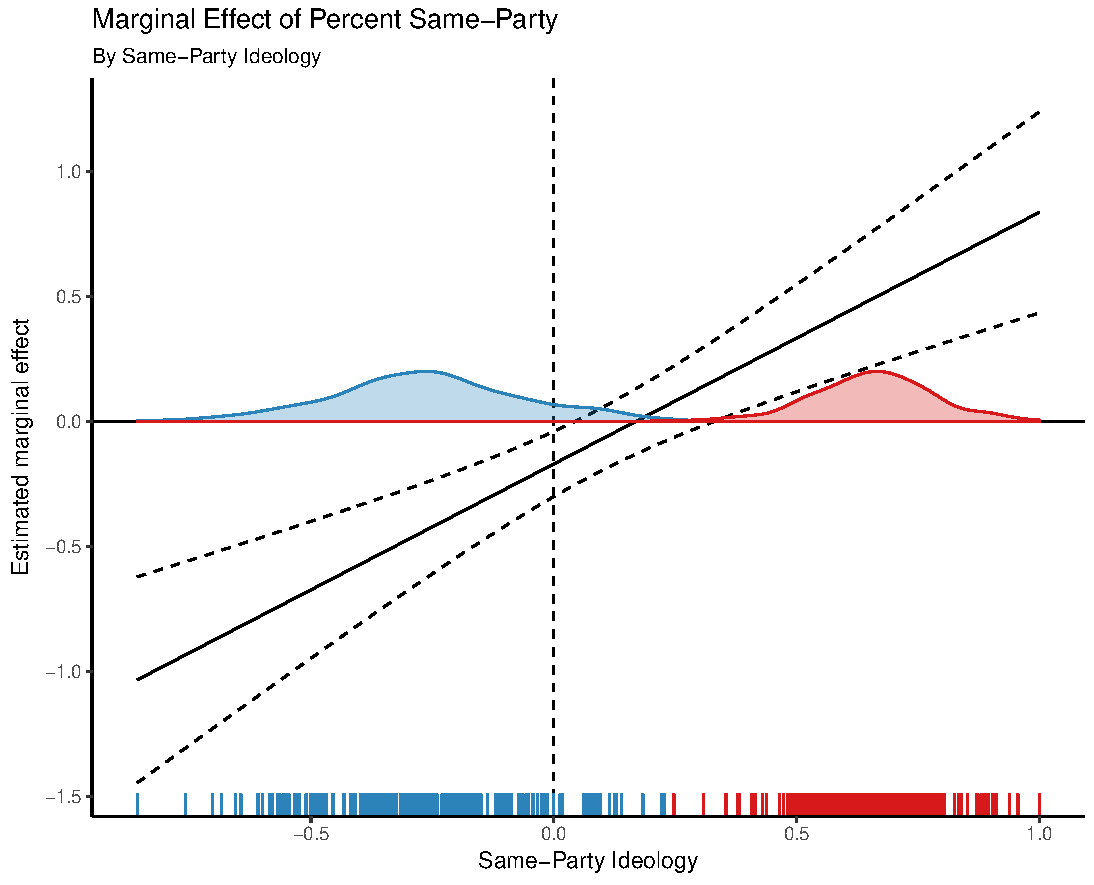
\includegraphics[width=.45\textwidth]{/Users/dsimp/GitHub/Clinton(2006)Rep/drafts/marginals/me-2.pdf} &
    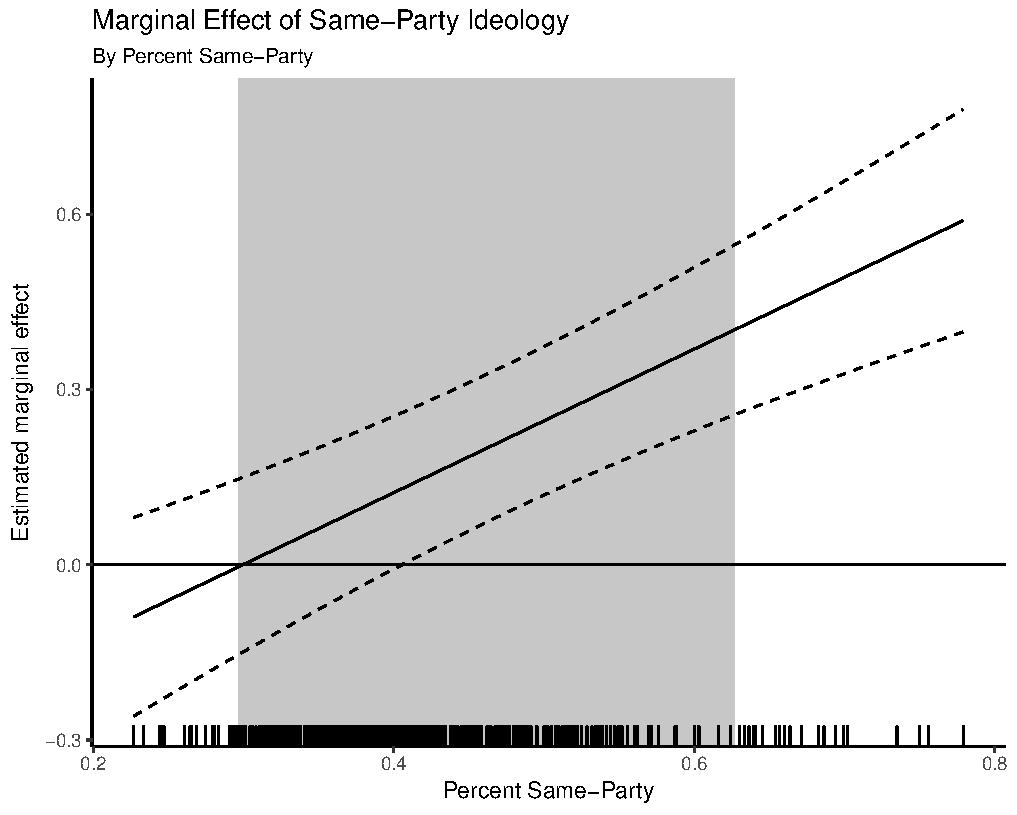
\includegraphics[width=.45\textwidth]{/Users/dsimp/GitHub/Clinton(2006)Rep/drafts/marginals/me-1.pdf} \\
     & \\
	\small (C) Marginal Effect of Percent Non-Same-Party& 
    \small (D) Marginal Effect of Non-Same-Party Ideology\\
    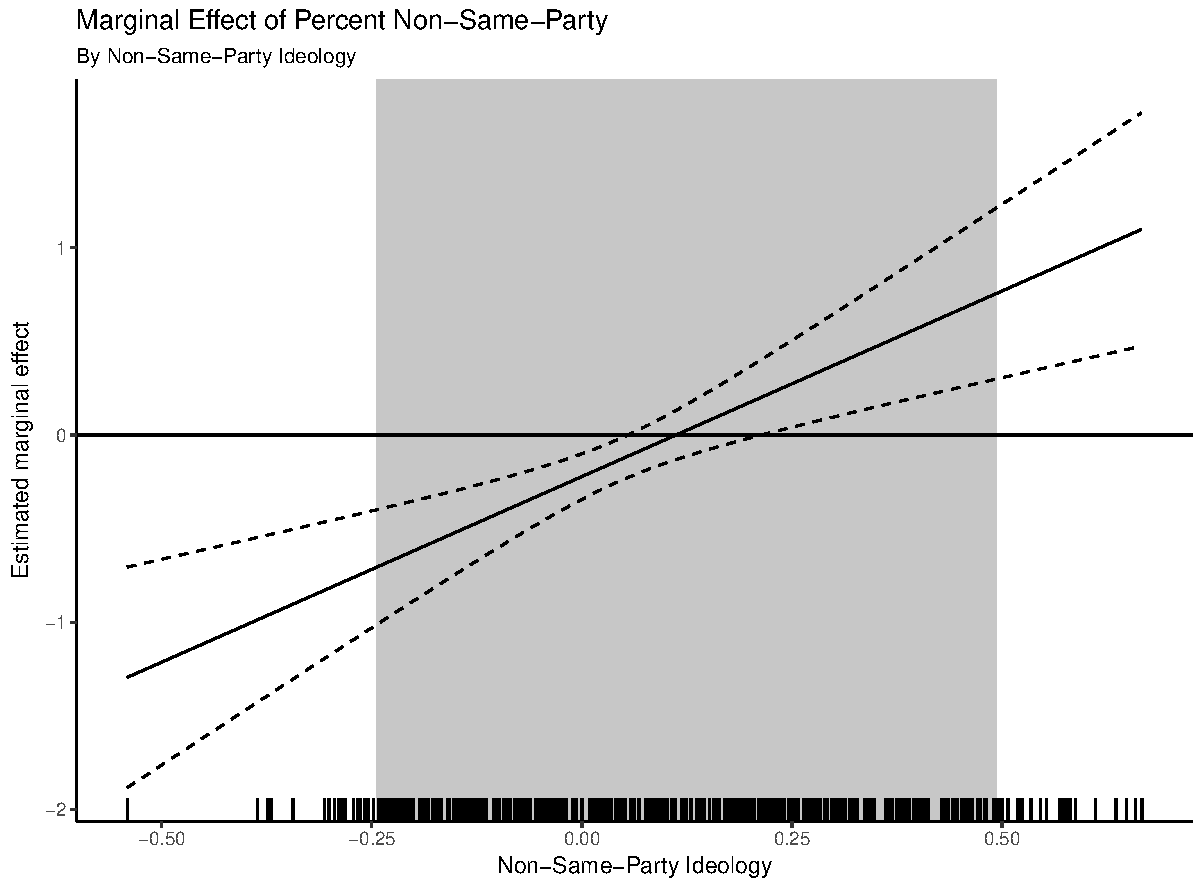
\includegraphics[width=.45\textwidth]{/Users/dsimp/GitHub/Clinton(2006)Rep/drafts/marginals/me-4.pdf} &
    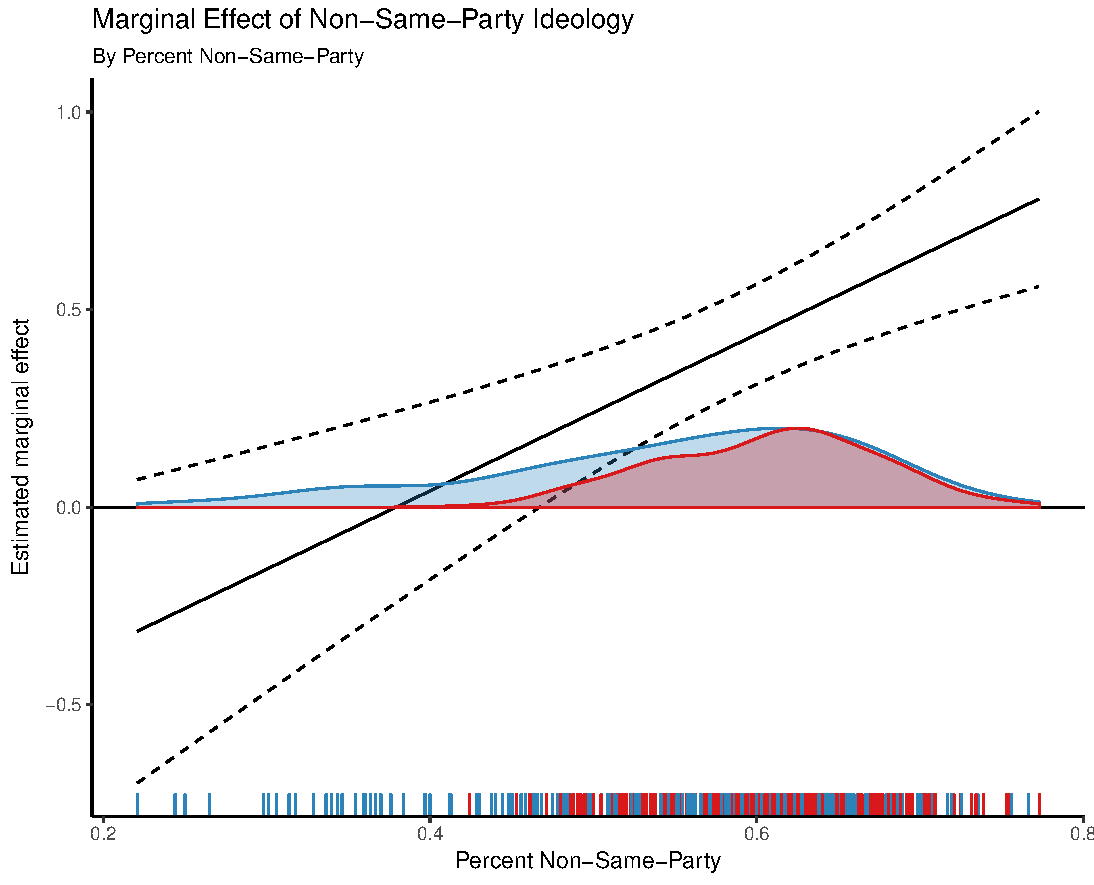
\includegraphics[width=.45\textwidth]{/Users/dsimp/GitHub/Clinton(2006)Rep/drafts/marginals/me-3.pdf} \\
     &  \\
  \end{tabular}
    %}   
 \end{centering}
  \textbf{Note:} Each panel plots the respective marginal effect of the constitutive terms of the interaction variables in Table 2 Model 3.
\end{figure}
 

\subsubsection{Transformations and Interpretation}


\cite{Gelman2007} argue that data transformations such as rescaling can be useful for coefficient interpretation. For example, mean centering data can improve interpretation when an independent variable value of zero does not make sense (p. 55). In this analysis, centering is relevant for variables such as group share, where no district has a sub-district group share value of zero. However, when the data is mean centered, the percent non-same-party variable drops from the regression due to multicollinearity. The results from this regression are shown in Table 1 model 4.  Therefore, to aid in interpretation, (future) Table X presents model 3 group share (ideology) coefficient estimates at various observed ideology (group) levels. \footnote{Will create and insert table in the next draft.}

\subsection{Ideology Scores - Two Groups or Three Groups}
To assess sub-district constituency influence on legislator behavior, \cite{Clinton2006} decomposes geographic constituency preferences into two weighted groups. The average ideology score $\bar{z}_i$ for each district $i$ is separated into the sample-population weighted same-party constituency preference $\frac{n_i^{SP}}{n_i}$ $\bar{z}_{SP_i}$ and the weighted non-same-party constituency preference $\frac{n_i^{NSP}}{n_i}$ $\bar{z}_{NSP_i}$. The decomposition is shown in the below equation (3). Recall $w_{SP_i} =\frac{n_i^{SP}}{n_i}$ and $w_{NSP_i} =\frac{n_i^{NSP}}{n_i}$.

\begin{equation}
\bar{z}_i = \bigg( \frac{n_i^{sp}}{n_i} \bigg) \bar{z}_{SP_i} + \bigg( \frac{n_i^{SP}}{n_i} \bigg) \bar{z}_{NSP_i}
\end{equation}
As stated above and shown in model (1), \cite{Clinton2006} regresses legislator ideal points on the district two group/party decomposition and legislators' party indicator variable. The previous section demonstrated the problems with failing to include the constitutive variables of the interaction terms. However, the decomposition into two rather than three groups poses an additional specification issue.

\textbf{Independent Lumping:} It is possible that partisan legislators are uniquely responsive to independents to the extent that independent constituents vote and are necessary for legislator victory in the 1998 midterm or 2000 presidential elections.
%Furthermore, one might expect that legislators in competitive districts uniquely compete more heavily for independent constituent votes than for opposite-party constituent votes. 
Figure 1, panel (I) demonstrates that, in general, independent constituents are ideologically closer to same-party constituents than opposite party constituents are to same-party constituents. \footnote{For example, in Democratic districts, independent voters span the range $[-0.50,0.50]$, yet the respective district opposite party voters are on average more conservative, with most scores falling in the range $[0.00,1.20]$.} \footnote{Similarly, in Republican districts independent voters are more conservative, with \textbf{Insert the comparison.}} As such, if legislators are responsive to independent and/or opposite party constituents at different share and ideology levels, it is possible that lumping the two groups into a single group could misrepresent the relationship between legislators and sub-district groups. Therefore, it is worth considering whether separating the district constituency into three sub-district groups will show that legislators are responsive to independent constituents and are more responsive to independents than opposite party constituents. To consider the individual effects of independents and opposite-party groups, I decompose the district ideology scores into weighted same-party $\frac{n_i^{SP}}{n_i}$ $\bar{z}_{SP_i}$, weighted independent voters $\frac{n_i^{I}}{n_i}$ $\bar{z}_{I_i}$, and weighted opposite-party $\frac{n_i^{OP}}{n_i}$ $\bar{z}_{OP_i}$. The new specification is shown in equation (3).
\begin{equation}
y_i  = \beta_0 + \beta_1 \bigg( \frac{n_i^{SP}}{n_i} \bigg) \bar{z}_{SP_i} + \beta_3 \bigg( \frac{n_i^{I}}{n_i} \bigg) \bar{z}_{I_i} + \beta_4 \bigg( \frac{n_i^{OP}}{n_i} \bigg) \bar{z}_{OP_i} + \gamma I_{GOP} + \varepsilon_i
\end{equation}

\textbf{Results:} The regression results from this equation are given in table 1 model 5. The high adjusted R-squared value indicates that model 5 explains most of the variation in legislator ideal points and more than the other considered models. The coefficient point estimates are almost all highly significant. However, it is necessary to turn to the marginal effects plots in Figure 4 to gain a holistic understanding of legislator responsiveness to sub-district group share and ideology. The same-party panels (A) and (B) are very similar to those in the Figure 3 two group analysis. \footnote{I need to add a coefficient estimate table for better interpretation and vertical lines to aid in visualization.} 

\textit{Independents:} Panels (C) and (D) provide analysis of independents. Panel (C) shows that the magnitude of the effect of independent share on legislator ideological consistency increases directly as independents become more polarized. Furthermore, as ideological extremity increases the impact of percent independent increases to a liberal value larger than the effect size of either percent same-party or percent non-same-party in the previous model 3 as depicted in Figure 3. Panel (D) indicates strong positive legislator responsiveness to independent ideology. As the percent of independents increases, the independent ideology has an increased positive/conservative effect on legislator ideological consistency.


\textit{Opposite Party:} Panel (E) also suggests legislators are highly responsive to the share of opposite party voters especially as the opposite party becomes more ideologically extreme. The associated relationship is also larger than what is suggested by the non-same-party results in model 3. Panel (F) depicts legislator responsiveness to opposite-party ideology. The plots suggests that at small opposite party shares, opposite party ideology is associated with negative/liberal ideological consistency. However, as opposite-party size increases, opposite party ideology is associated with increases in positive/conservative ideological consistency. \footnote{As with the previous section, I have some interpretation questions here.} \textbf{Maybe insert comment about needed to use two groups and three group to augment analysis.}

\textbf{Discussion:} Figure 4 provides strong evidence that the non-same-party variable is a function of two unique group variables that have distinct relationships with legislator ideal points. As such, more work may be necessary to justify the use of two groups rather than three groups analysis in sub-district analysis. Alternatively, it may be necessary to at a minimum use both two group and three analysis to gain a better understanding of legislator responsiveness to sub-district ideology. The group share marginal effects plots (Panel C and E) show that legislator responsiveness to independents and opposite party constituents follow different paths. The distributions in panel (C) seem to suggest increased responsiveness at liberal ideologies rather than conservative ideologies. The distributions plotted in panel (E) seem to suggest both parties are responsive to opposite party constituents.\footnote{To the left of the vertical zero line, all districts are Republican held; to the the right, most districts are Democratic held. Yet, the plot indicates a high degree of legislator responsiveness to the ideology of opposite-party constituents at both increased liberal and conservative ideologies. The plot suggests that as polarization increases, the opposite party share is associated with a larger decline in the legislator's party based ideological consistency.} Compared to the non-same party plot in Figure 3 panel (C), the opposite party Figure 4 panel (E) plot shows a high level of responsiveness to ideologically extreme conservative opposite party constituents. Furthermore, panels (C) and (E) shows high degree of responsiveness to both ideological extremes.

In this proposal, I do not provide an in depth discussion of why legislators are responsive to opposite party constituents. A potential reason could be coincidental responsiveness. Coincidental responsiveness could occur if changes in opposite-party share and ideology are highly correlated with changes in same-party and independent share  and ideology.  As illustrated by the multicollinearity discussion, opposite-party share is highly correlated with same-party and independents shares. Across all districts, the relationship between district conservatism and opposite party conservatism by party is positive. A second potential source of this observed relationship is the relationship among district competitiveness and group share and ideology. Many districts have large opposite party group shares. For example, Figure 1 panel (D) shows that many Democratic districts have an ideology more conservative than the average Republican held district. For a Democrat to compete in a conservative district, competition for independents may require adopting policies supported by conservative constituents.

\textbf{Summary:} This section finds that legislators are uniquely responsive to independents and to opposite party constituents. Such evidence should raise debate over whether it is valid to lump independents with opposite party constituents to form a non-same party group.
\begin{figure}[!htbp]
\caption{Representative Ideal Points and District Ideology (Three Groups)}
\begin{centering}
%\centering
%\fbox{
  \begin{tabular}{@{}cc@{}}
	 & \\  	
	\small (A) Marginal Effect of Percent Same-Party&	
  	\small (B) Marginal Effect of Same-Party Ideology\\
    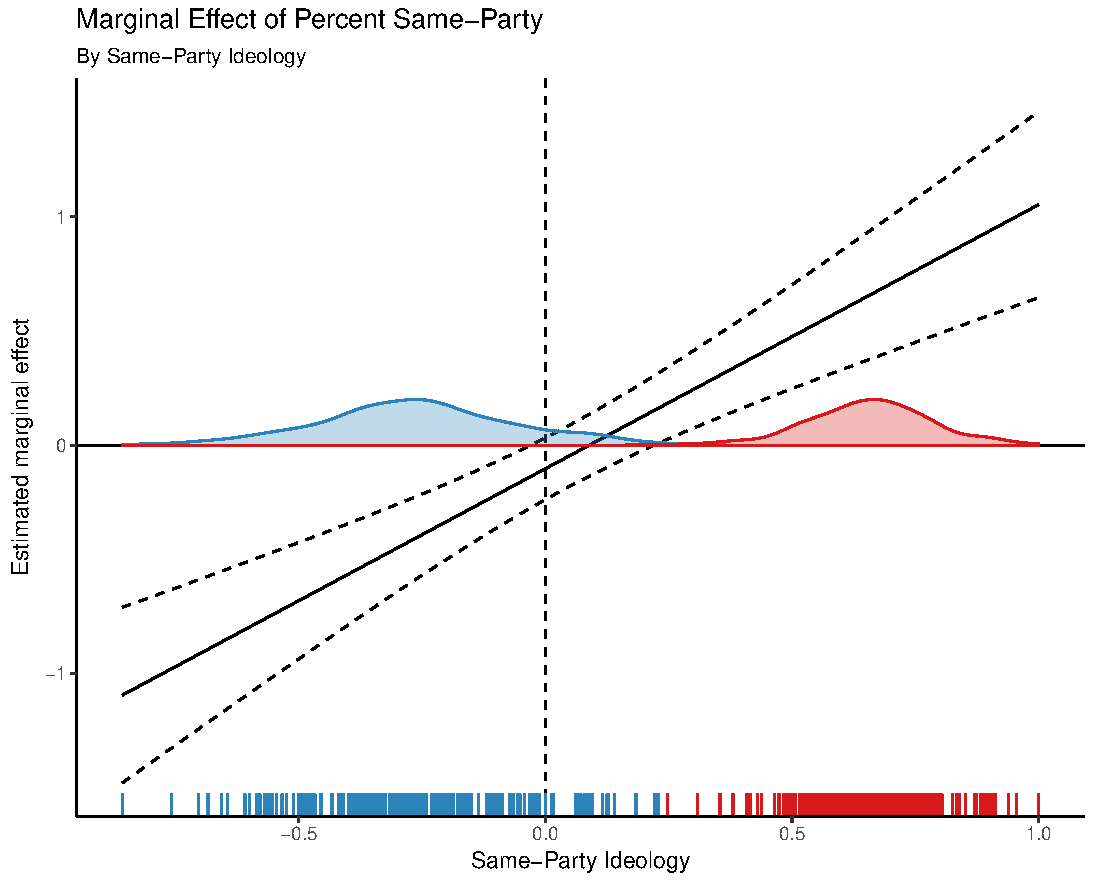
\includegraphics[width=.45\textwidth]{/Users/dsimp/GitHub/Clinton(2006)Rep/drafts/marginals/meb-1.pdf} &
    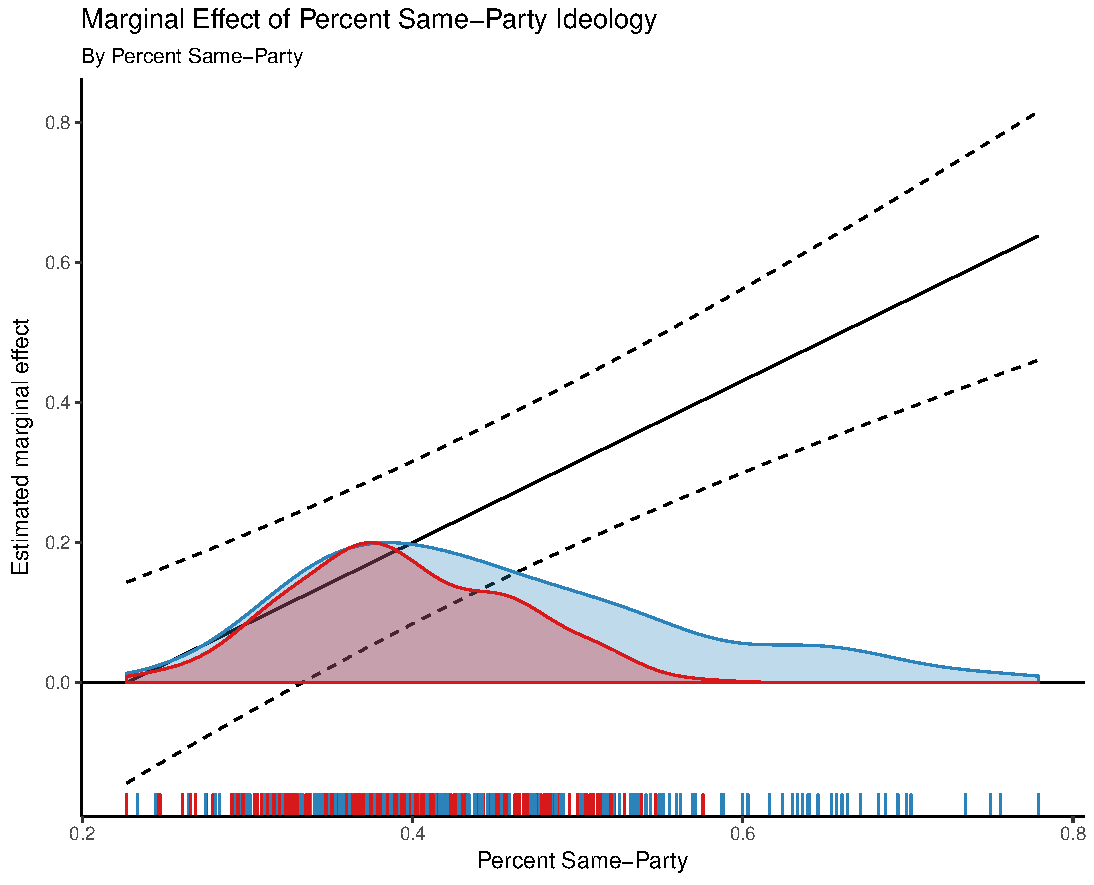
\includegraphics[width=.45\textwidth]{/Users/dsimp/GitHub/Clinton(2006)Rep/drafts/marginals/meb-2.pdf} \\
     & \\
	\small (C) Marginal Effect of Percent Independent& 
    \small (D) Marginal Effect of Independent Ideology\\
    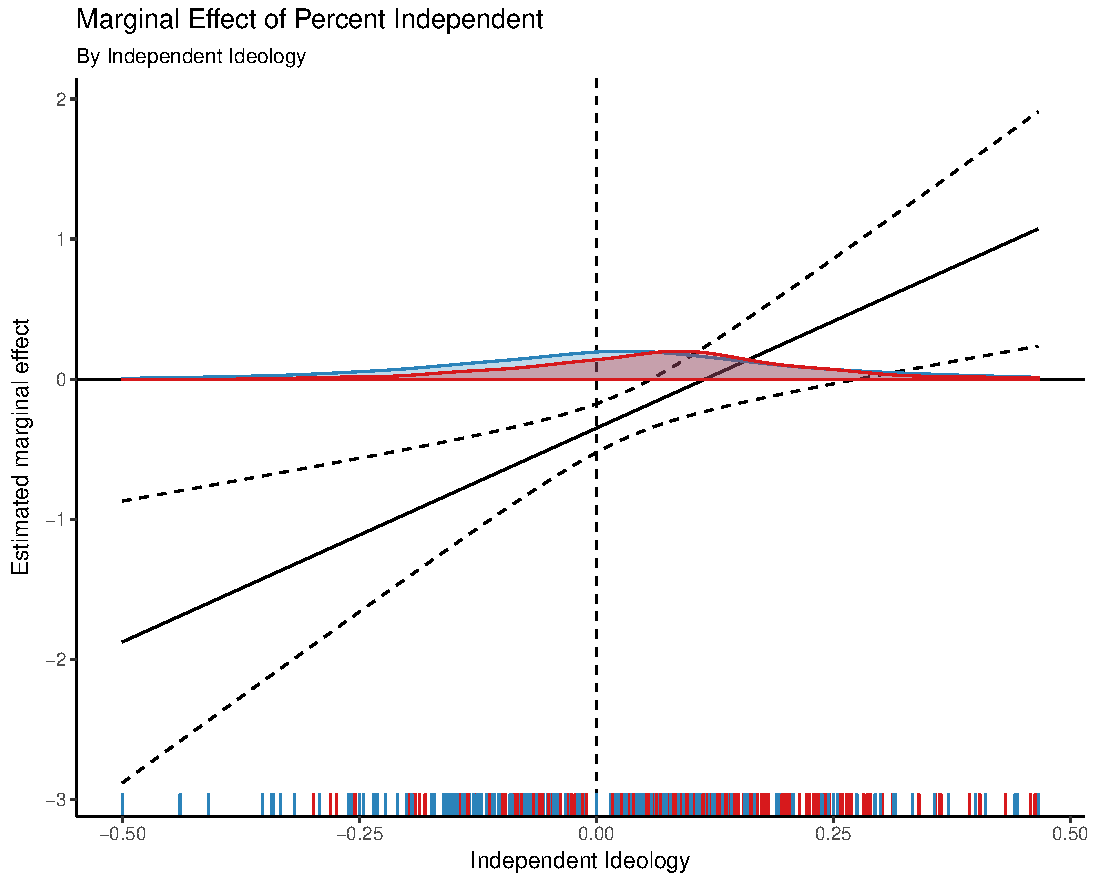
\includegraphics[width=.45\textwidth]{/Users/dsimp/GitHub/Clinton(2006)Rep/drafts/marginals/meb-3.pdf} &
    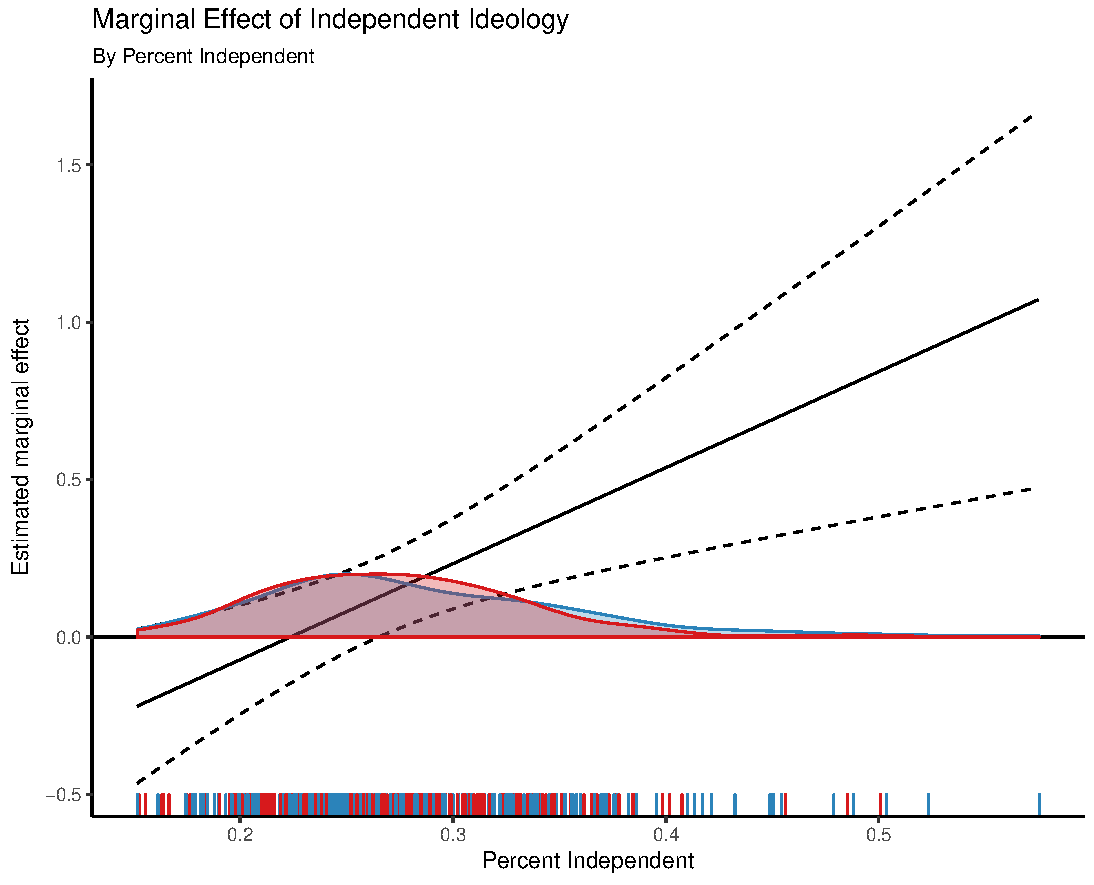
\includegraphics[width=.45\textwidth]{/Users/dsimp/GitHub/Clinton(2006)Rep/drafts/marginals/meb-4.pdf} \\
     &  \\
    \small (E) Marginal Effect of Percent Opposite-Party&  
    \small (F) Marginal Effect of Opposite-Party Ideology\\
    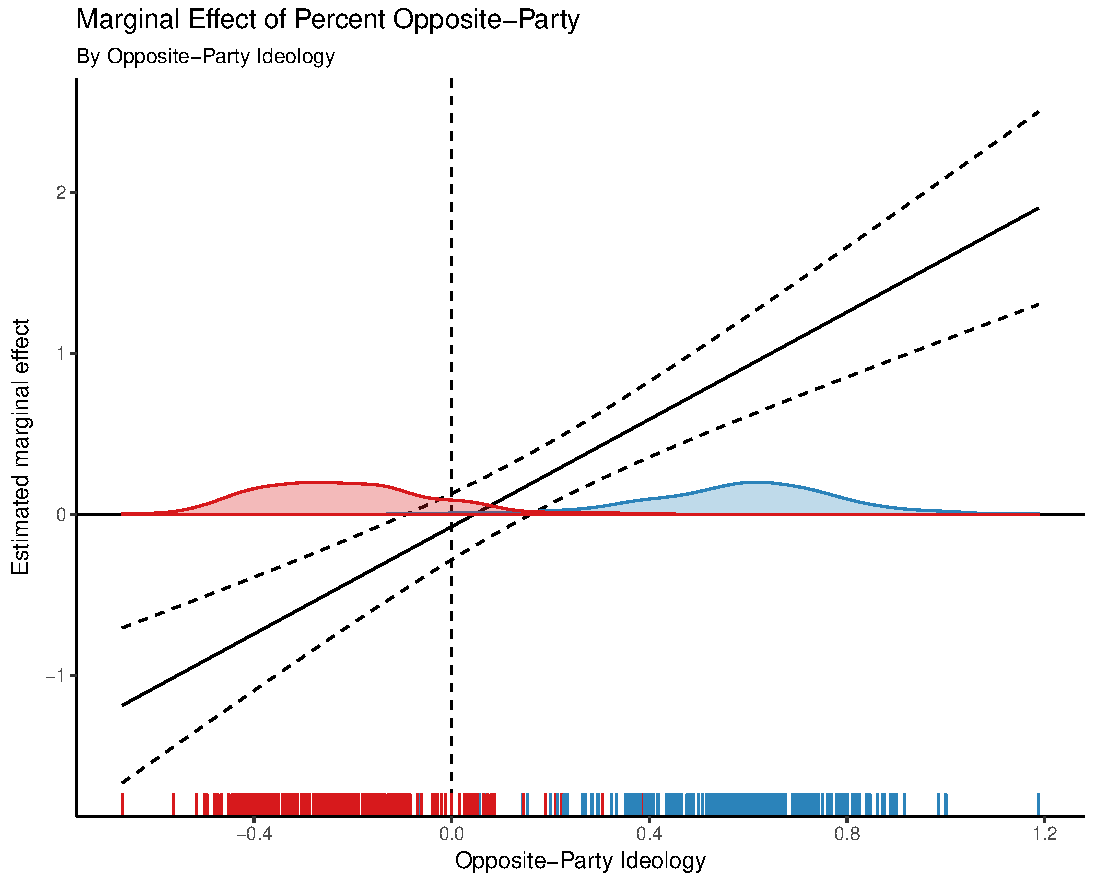
\includegraphics[width=.45\textwidth]{/Users/dsimp/GitHub/Clinton(2006)Rep/drafts/marginals/meb-5.pdf} &
    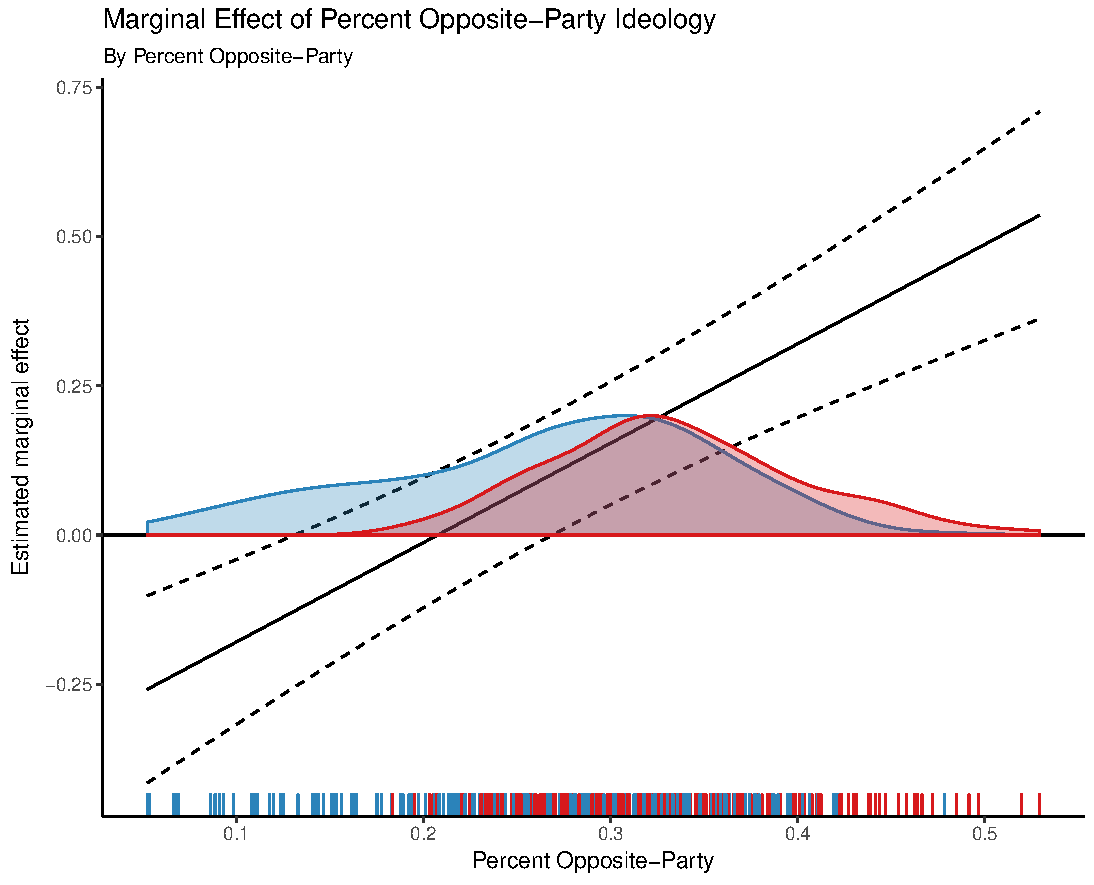
\includegraphics[width=.45\textwidth]{/Users/dsimp/GitHub/Clinton(2006)Rep/drafts/marginals/meb-6.pdf} \\
     &  \\
  \end{tabular}
    %}   
 \end{centering}
  \textbf{Note:} Each panel plots the respective marginal effect of the constitutive terms of the interaction variables in Table 2 Model 5.
\end{figure}
 

\newpage
\begin{figure}[!htbp]
\caption{District Group and Legislator Vote Distribution (All Votes)}
\begin{centering}
%\centering
%\fbox{
  \begin{tabular}{c}%{@{}ccc@{}}
    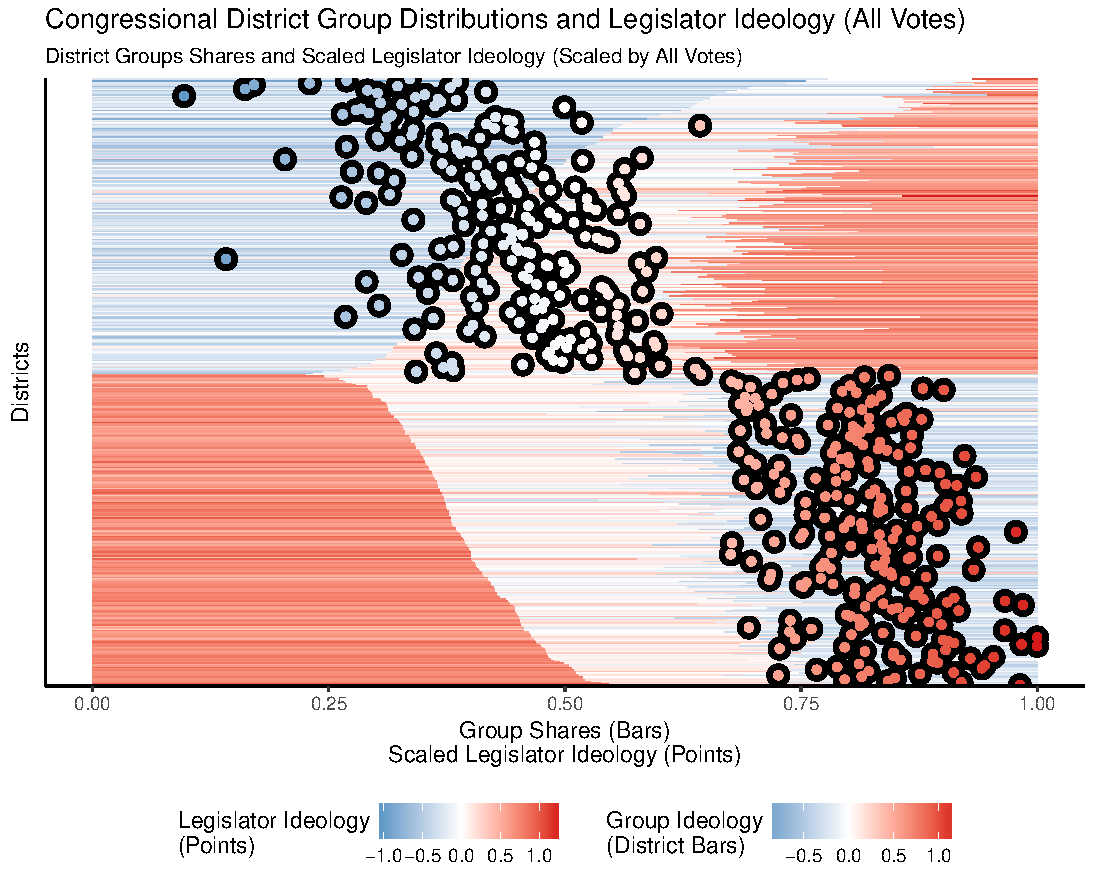
\includegraphics[width=.80\textwidth]{/Users/dsimp/GitHub/Clinton(2006)Rep/drafts/compare/compare1}\\
    \\
    \\
    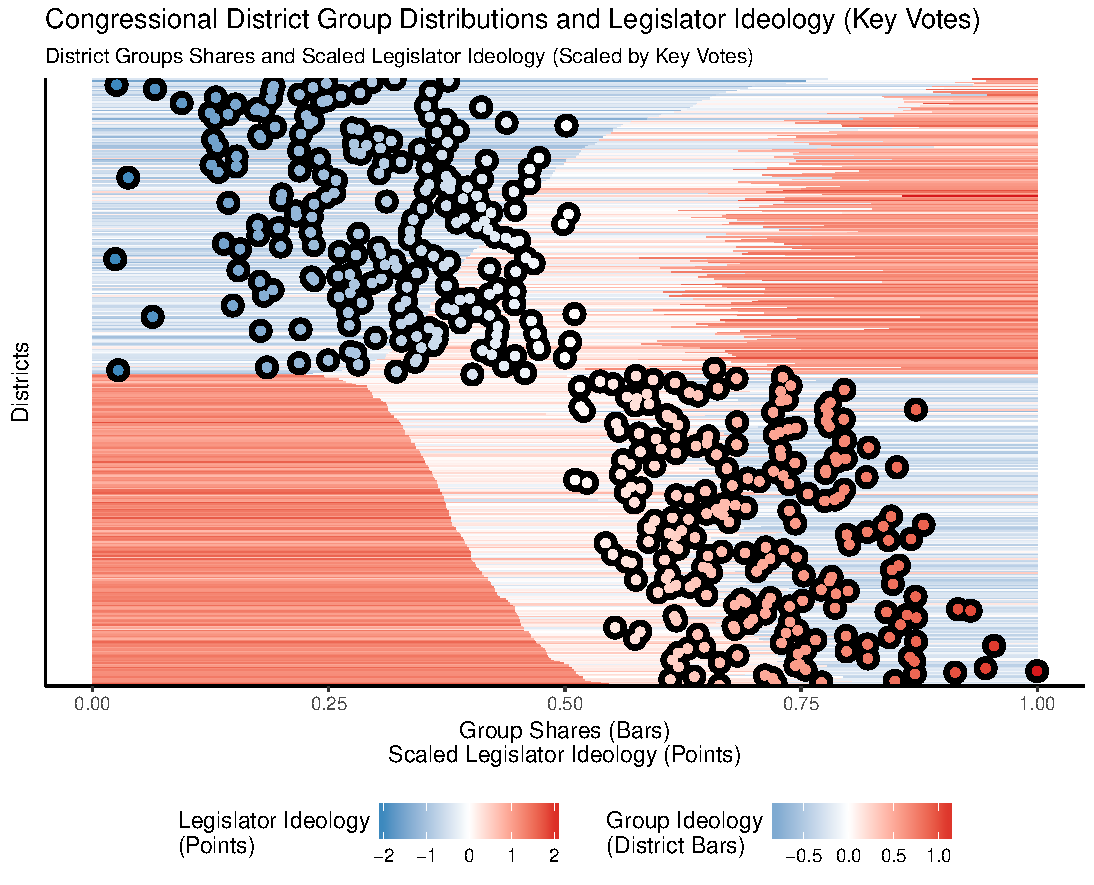
\includegraphics[width=.80\textwidth]{/Users/dsimp/GitHub/Clinton(2006)Rep/drafts/compare/compare2}\\
    %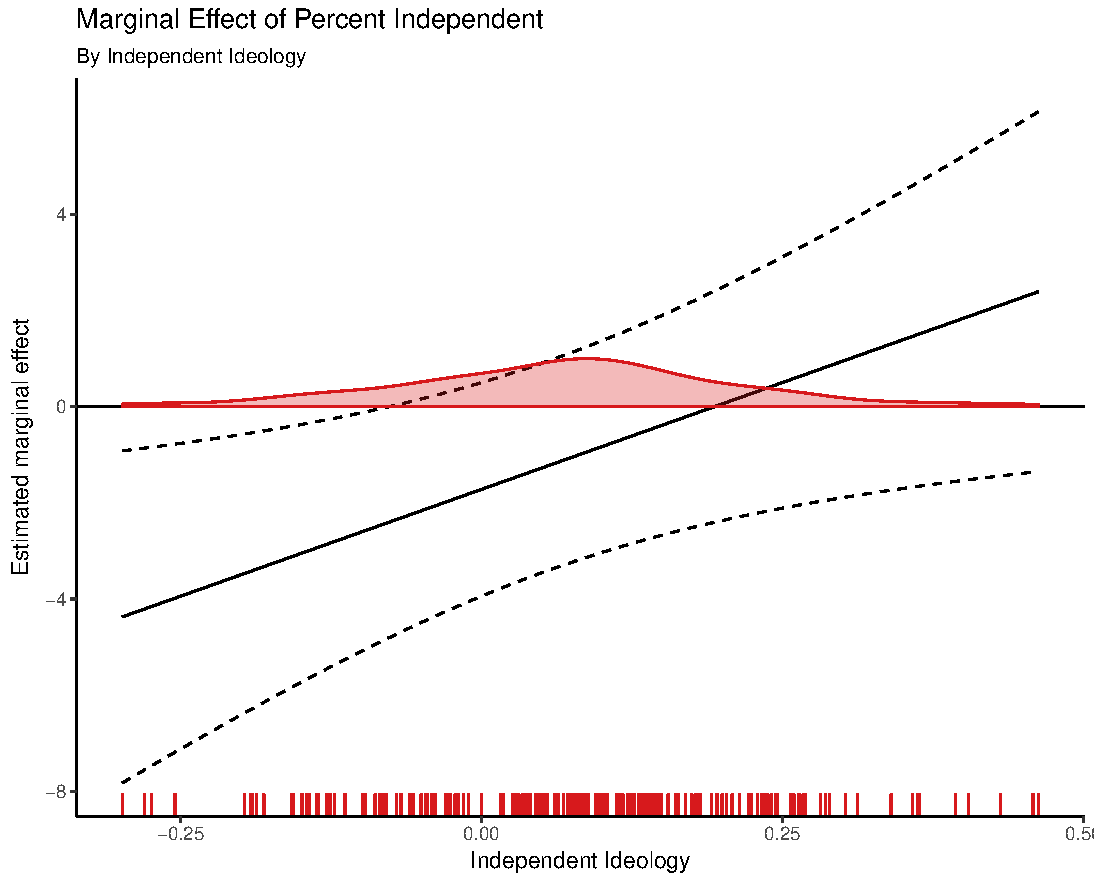
\includegraphics[width=.25\textwidth]{/Users/dsimp/GitHub/Clinton(2006)Rep/drafts/marginals/me4-3}
  \end{tabular}
    %}   
 \end{centering}\\
  %\textbf{Note:} Words 
\end{figure}

\newpage

\subsection{Resolving the Responsiveness Puzzle: Party Analysis with All Votes} The responsiveness puzzle is based on analysis of districts by party control and it suggests Republican legislators are responsive to the preferences of same-party constituents whereas Democratic legislators are responsive to their non-same party constituents. Clinton (2006) argues that analysis of the entire House rather than analysis by party can produce misleading results due to averaging party based differences (p. 404). Similarly, I split the data by district party control to consider ideal point variation within each party. Table 3 presents legislator ideal point responsiveness to sub-district groups. In theses models, the data is split into a Republican set and a Democratic set. Models 1 through 3 provide regressions across Republican held districts. Models 4 through 6 are regressions across Democratic held districts.

\textbf{EIV Analysis:} Models 1 and 4 are identical replications of Clinton's OLS analysis of Republican and Democratic districts. These models fail to include the constitutive terms and should not be used for analysis. To argue in favor of the responsiveness puzzle, Clinton considers an EIV specification of the table 3 models 1 and 4. I am able to reproduce these models in STATA, though I have not reported them here. Clinton argues for the responsiveness puzzle since the EIV models shows that the only coefficient on weighted same-party ideology is significant for Republicans and only the coefficient on weighted non-same-party ideology is significant for Democrats. However, as discussed one cannot infer the relationship among these variable in either the OLS or EIV regression without including the constitutive terms. I have attempted to run the EIV regression with the constitutive terms but STATA returns a model specification error. In the next draft I plan to provide a more extensive analysis of the EIV  models and STATA's EIV package.

\textbf{OLS Analysis:} Table 3 also provides the results for the unbiased specified OLS two group and three group models. The unbiased two group models 2 and 5 illustrate the dramatic improvement in model fit over the biased underspecified models 1 and 4. There is a considerable improvement in the adjusted R squared for both of these models. Readers should refrain from directly interpreting the coefficient values without directly calculating the marginal effects of group share and ideology. The results of the three group analysis are presented in models 3 and 6 and the respective marginal effects plots are given in Figure 6.

\textit{Same-Party:} The Figure 6 panels (A) and (G) provide the respective marginal effects plots of same-party share for Republicans and Democrats. Panel A indicates that Republican legislators are responsive to percent same-party at low ideology levels and that the effect increases with conservative ideological extremity. In contrast, panel G illustrates a weak relationship between percent same party and legislator ideological consistency in Democratic districts with higher levels of liberal ideology. However, as ideology is less extreme, percent same party is associated with an increased liberal ideological consistency. It is possible that the plots show Republicans (Democrats) have increasing (decreasing) returns to ideological extremity in the same party share plots. However, more theoretical work is needed to explain this finding. 

Panel (D) (panel (J)) shows that in Republican (Democratic) districts same-party ideology is associated with increased (decreased) conservative ideological consistence as percent same party increases. For Republicans, as the percent same-party increases the associated impact of ideology on legislator conservative ideology increases. Yet is is only significant along a small range. For Democrats, as the percent same-party increases the associated impact of ideology on legislator ideology is positive and conservative but decreases.

\textit{Independents:} Pots (B) and (H) show that the relationship between percent independents and ideological consistency is negative at liberal ideologies and becomes positive at conservative ideologies. The slope of the Republican plot is steeper than that of the Democratic plot. (In the next raft, I will rescale the axes to provide a more nuanced responsiveness and congruence discussion). Plots (E) and (K) show that the relationship between independent ideology and legislator ideological consistency suggests that as the share of independents increases, the observed relationship between ideology and ideological consistency is more positive.

\textit{Opposite Party:} Panels (C) and (I) show both parties are responsive to opposite party share. Furthermore, they show a strong positive relationship between opposite party share and conservative ideological consistency when opposite party ideology moves toward conservative extremity. Panels (F) and (L) suggest that as opposite party share increases the associated relationship between \textbf{X and Y} becomes more positive/conservative. However, note that at low levels of opposite party size \textbf{blah.}


\textbf{Responsiveness Puzzle:} The party based all votes analysis provides no support for the responsiveness puzzle. Since the puzzle was observed under a biased underspecified model and cannot be supported under unbiased analysis, it should be disregarded in the literature. Rather, the Figure 6 plots show legislators are responsive to same-party constituents and have \textbf{varying} degrees of significant responsiveness to independents and opposite party constituents. \footnote{The OLS results show GOP responsiveness to the size and ideology of their same-party, independent and opposite party constituents. The findings suggest similar significant results for Democratic legislators; however, the relationship for independents is not significant.} Additional work is required to explain the observed relationships.

\textbf{Summary:} This sections has provided strong evidence to contradict the responsiveness puzzle. 

\input{/Users/dsimp/GitHub/Clinton(2006)Rep/drafts/stargazer/table3.txt}

% Interaction Terms All Votes
\begin{figure}[!htbp]
\caption{Marginal Effects of Interaction Terms (All Votes)}
\begin{centering}
%\centering
%\fbox{
  \begin{tabular}{ccc}%{@{}ccc@{}}
	& \small \textbf{GOP Regression} & \\ 
	& & \\ 	
  	\small (A) Percent Same-Party& 
  	\small (B) Percent Independent& 
    \small (C) Percent Opposite-Party\\
    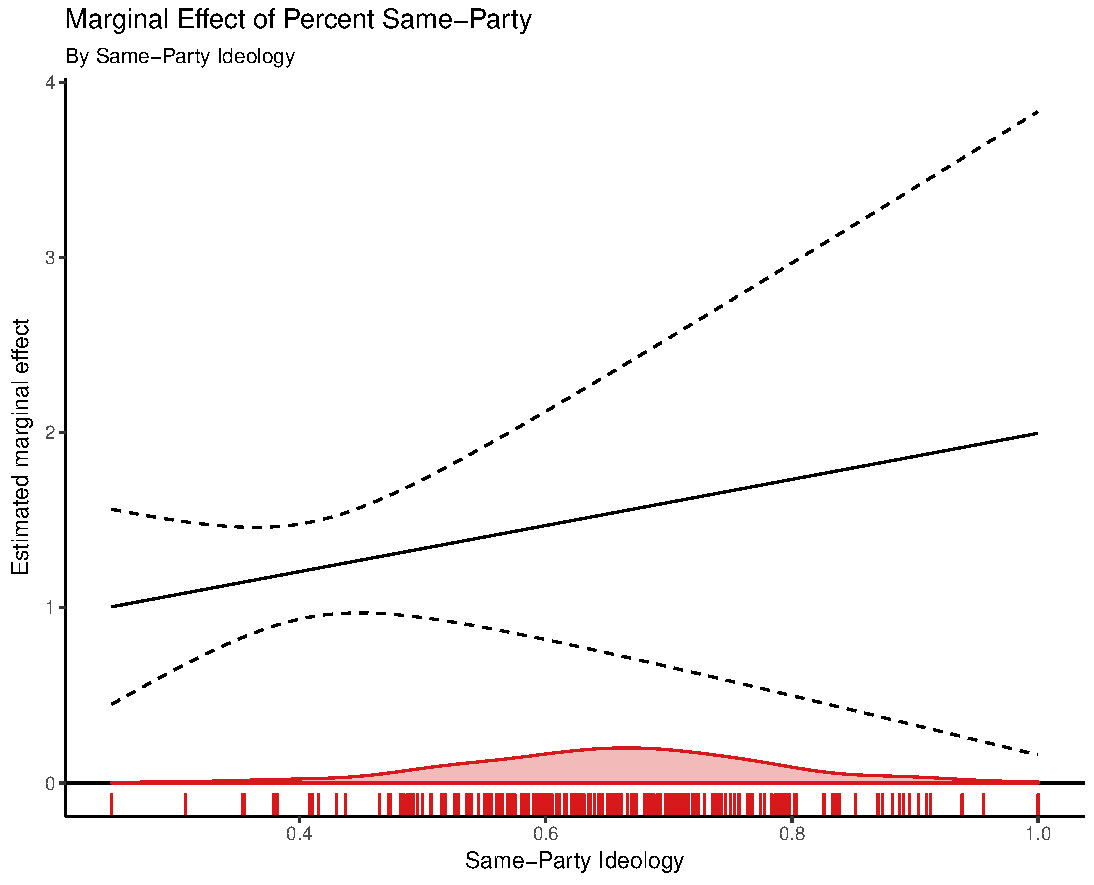
\includegraphics[width=.25\textwidth]{/Users/dsimp/GitHub/Clinton(2006)Rep/drafts/marginals/me2-1} &
    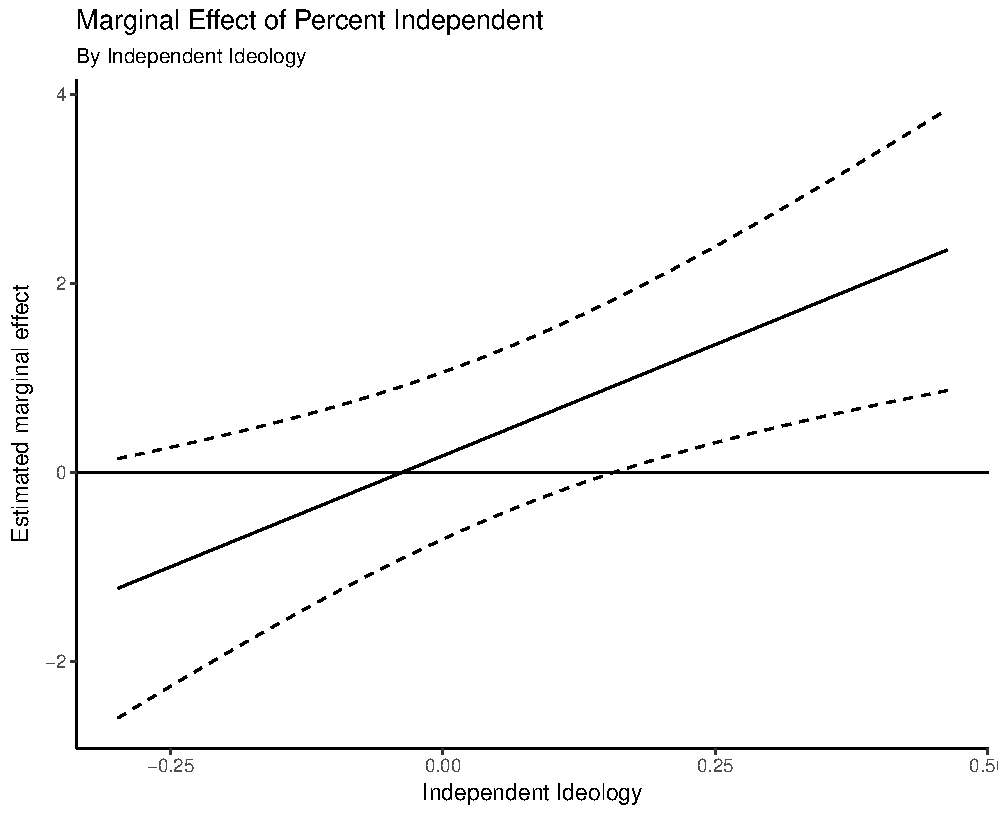
\includegraphics[width=.25\textwidth]{/Users/dsimp/GitHub/Clinton(2006)Rep/drafts/marginals/me2-3} &
    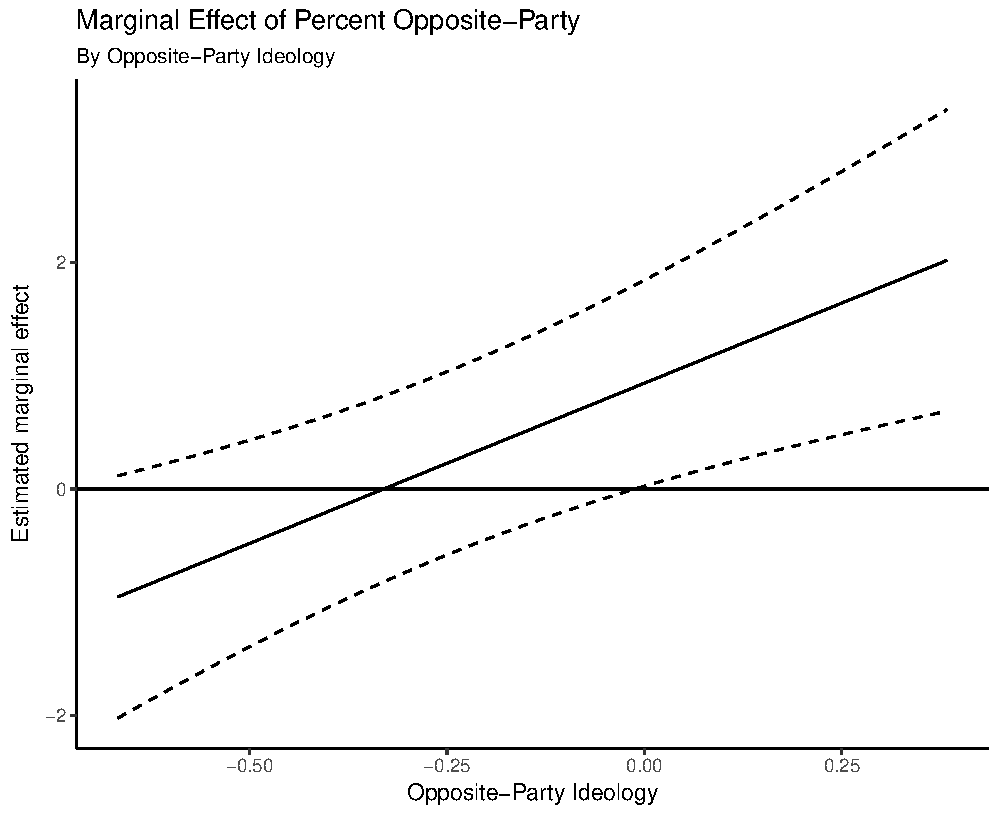
\includegraphics[width=.25\textwidth]{/Users/dsimp/GitHub/Clinton(2006)Rep/drafts/marginals/me2-5} \\
     & & \\
  	\small (D) Same-Party Ideology& 
  	\small (E) Independent& 
    \small (F) Opposite-Party Ideology\\
    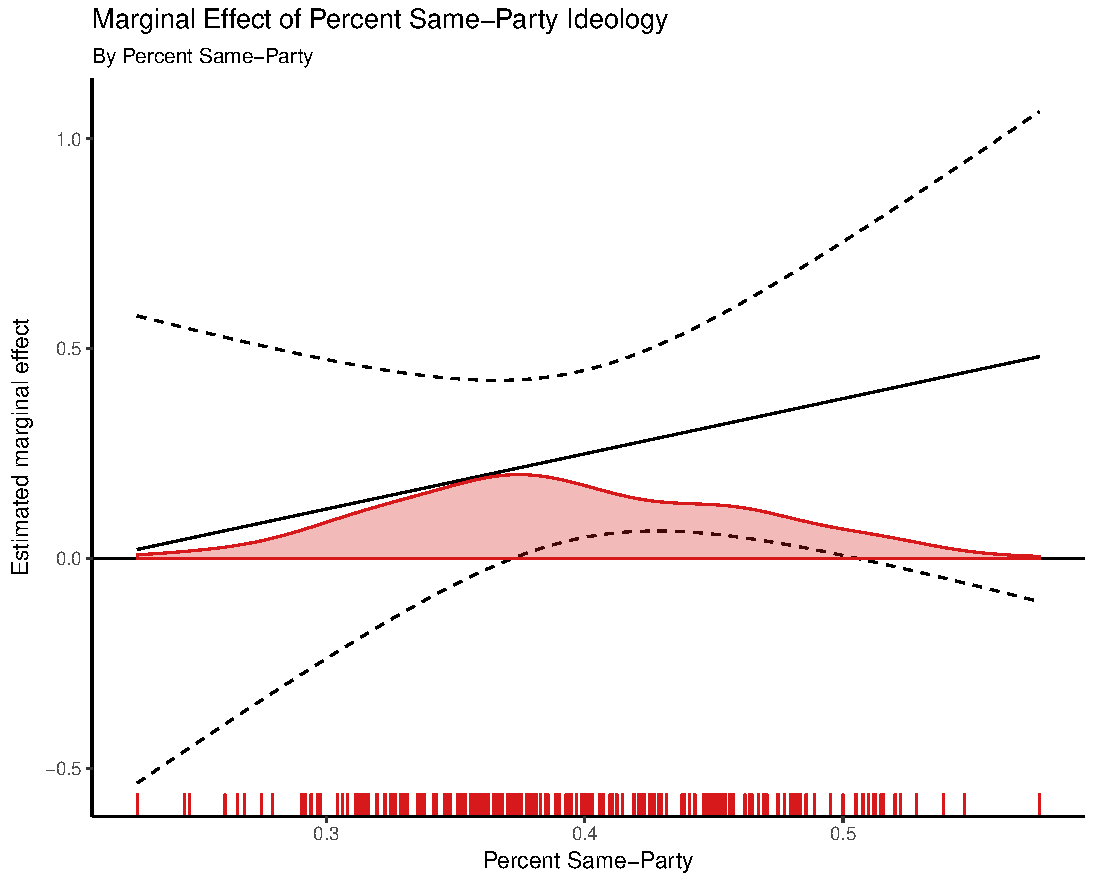
\includegraphics[width=.25\textwidth]{/Users/dsimp/GitHub/Clinton(2006)Rep/drafts/marginals/me2-2} &
    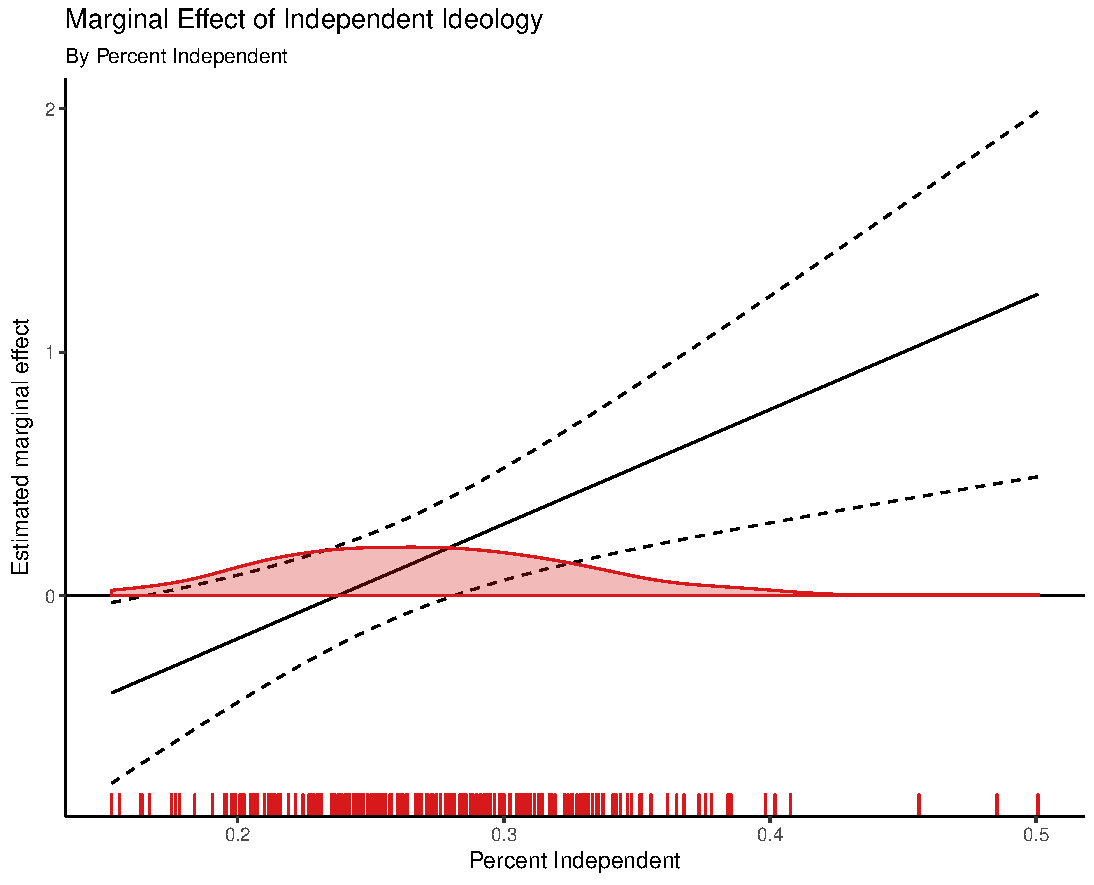
\includegraphics[width=.25\textwidth]{/Users/dsimp/GitHub/Clinton(2006)Rep/drafts/marginals/me2-4} &
    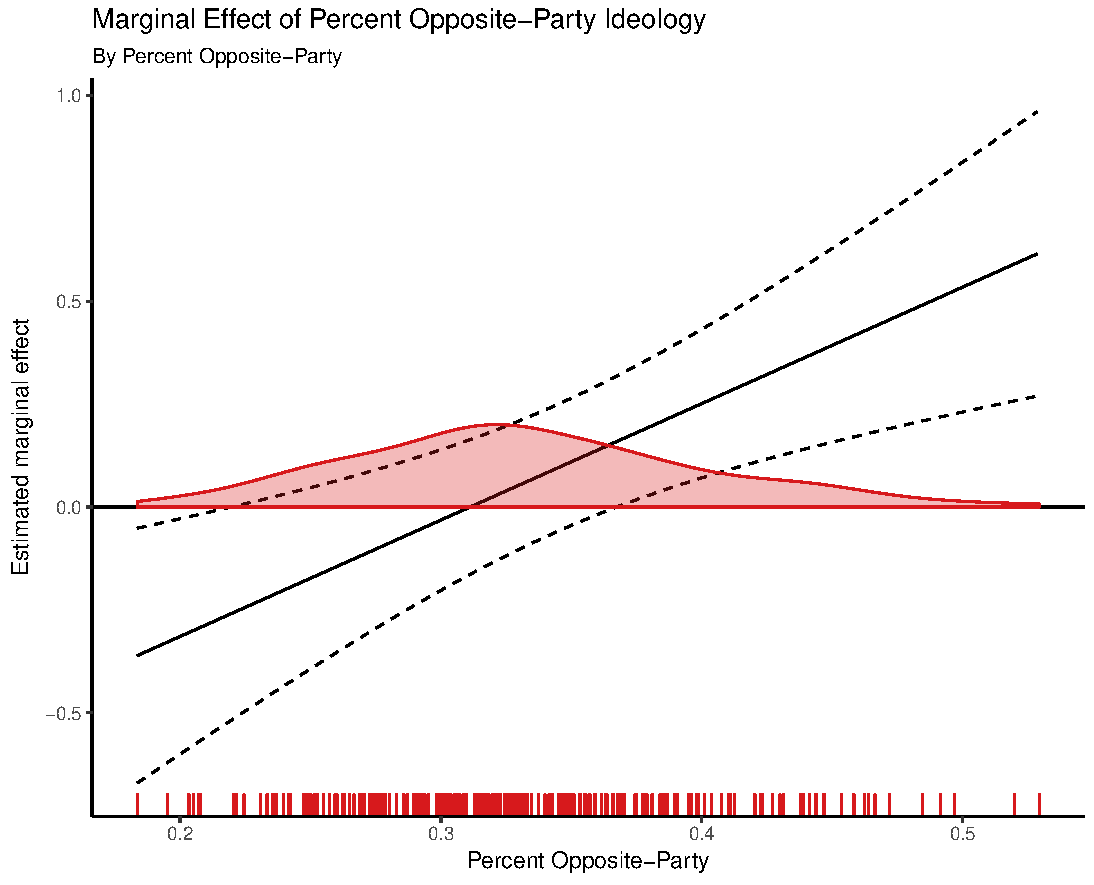
\includegraphics[width=.25\textwidth]{/Users/dsimp/GitHub/Clinton(2006)Rep/drafts/marginals/me2-6} \\
    	& & \\ 
	& \small \textbf{DEM Regression} & \\ 
	& & \\ 
  	\small (G) Percent Same-Party& 
  	\small (H) Percent Independent& 
    \small (I) Percent Opposite-Party\\
    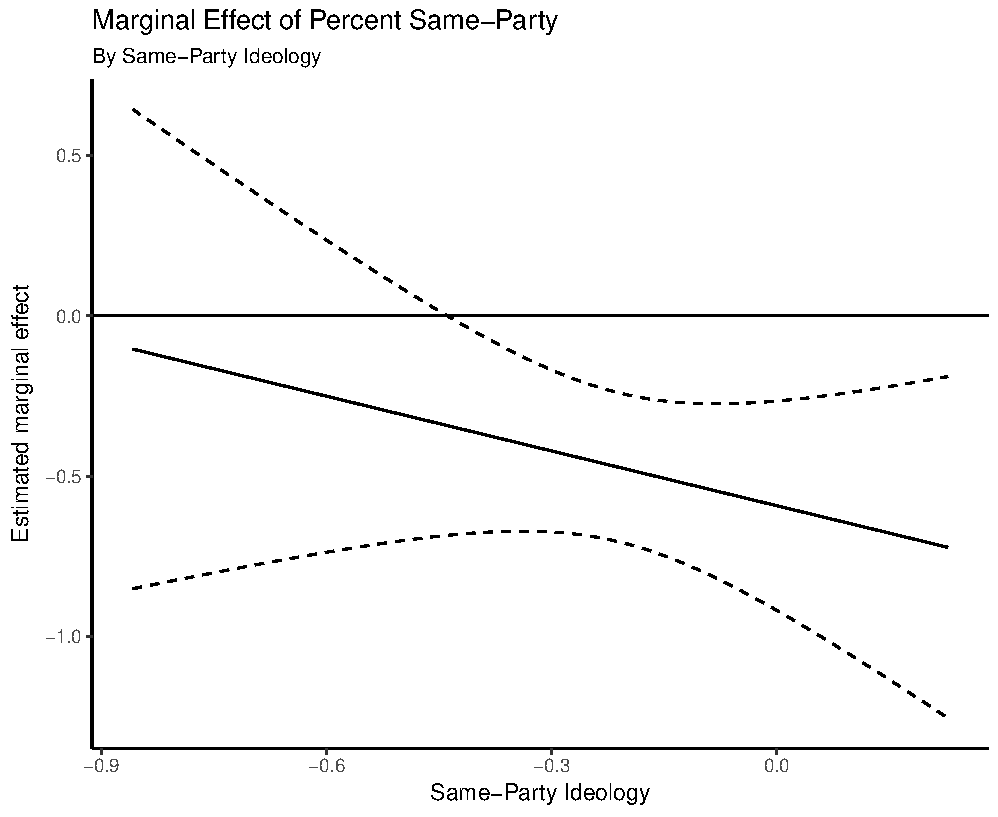
\includegraphics[width=.25\textwidth]{/Users/dsimp/GitHub/Clinton(2006)Rep/drafts/marginals/me3-1} &
    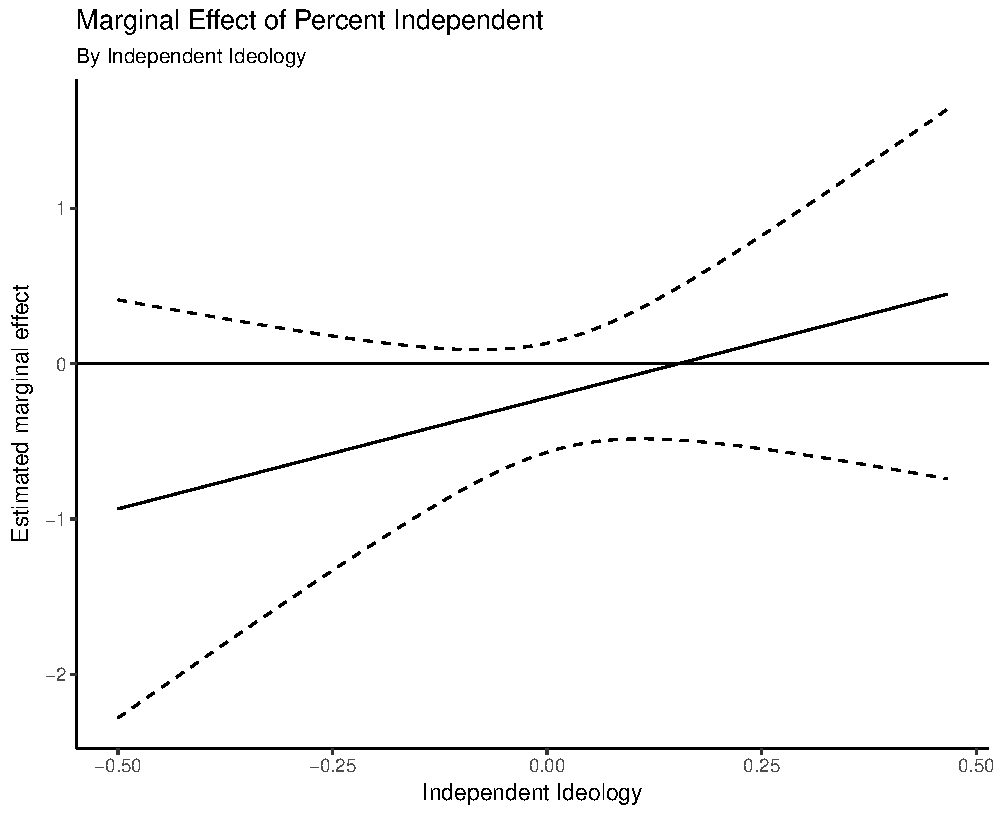
\includegraphics[width=.25\textwidth]{/Users/dsimp/GitHub/Clinton(2006)Rep/drafts/marginals/me3-3} &
    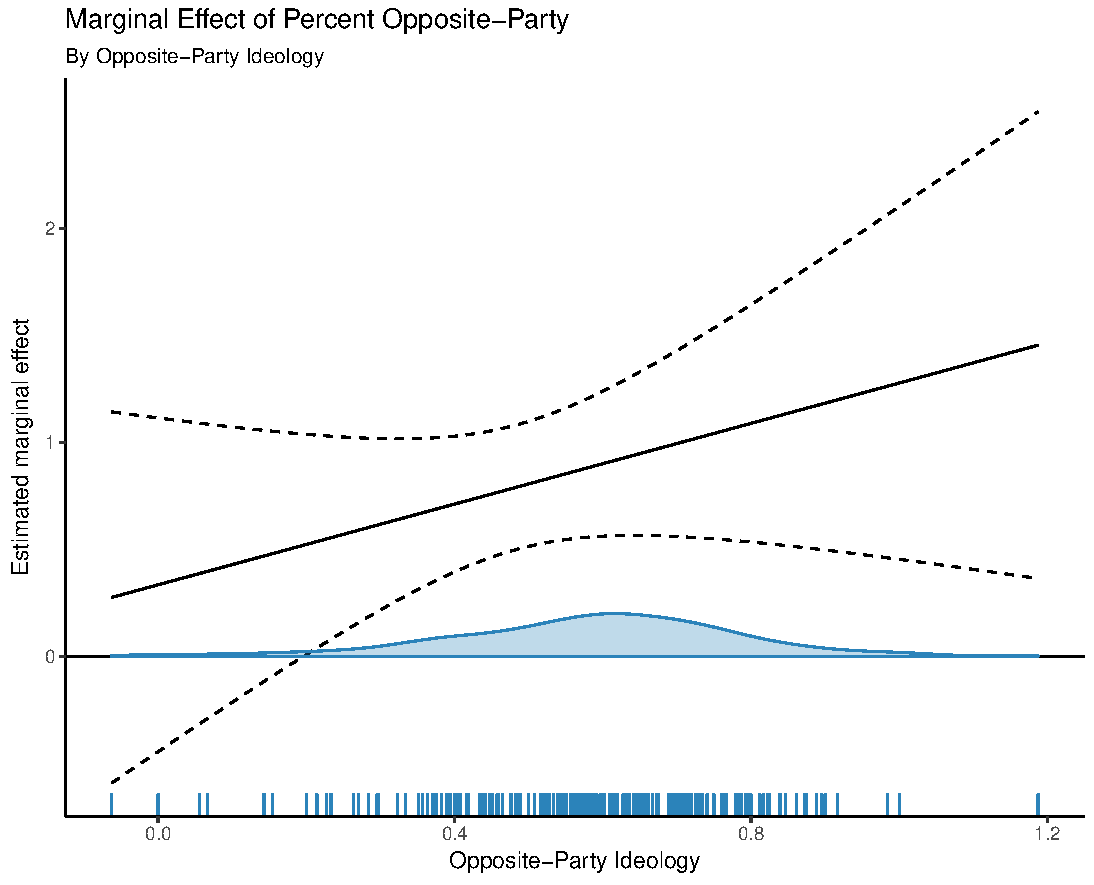
\includegraphics[width=.25\textwidth]{/Users/dsimp/GitHub/Clinton(2006)Rep/drafts/marginals/me3-5} \\
     & & \\
  	\small (J) Same-Party Ideology& 
  	\small (K) Independent Ideology& 
    \small (H) Opposite-Party Ideology\\
    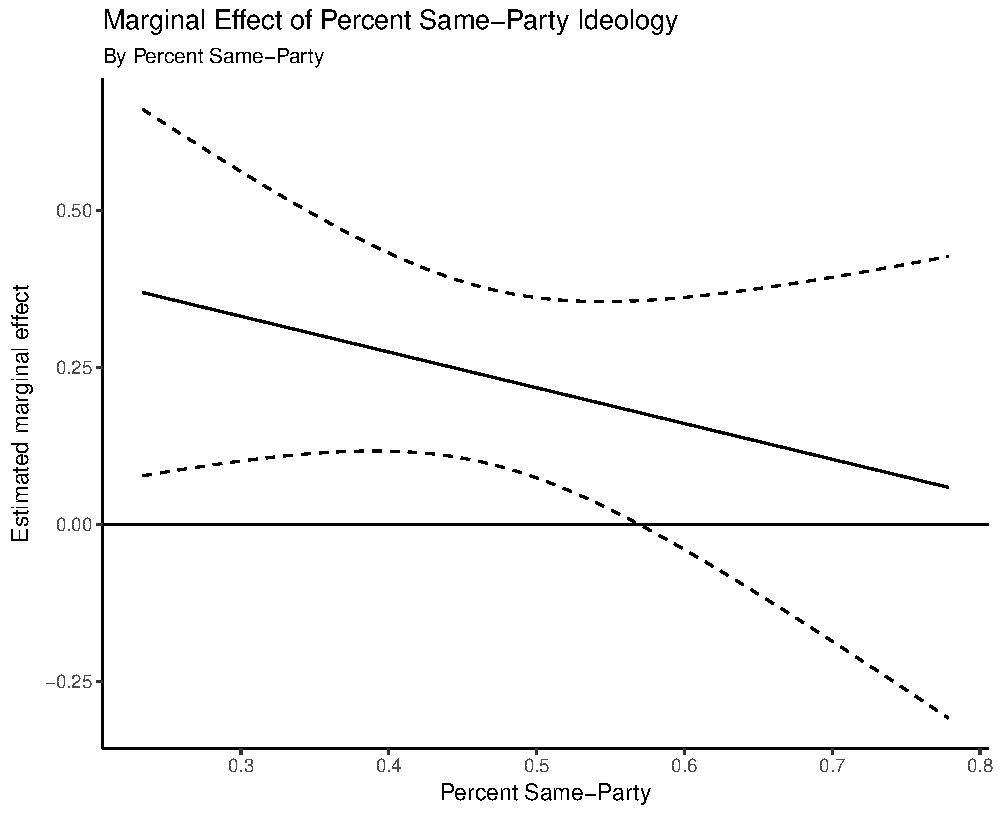
\includegraphics[width=.25\textwidth]{/Users/dsimp/GitHub/Clinton(2006)Rep/drafts/marginals/me3-2} &
    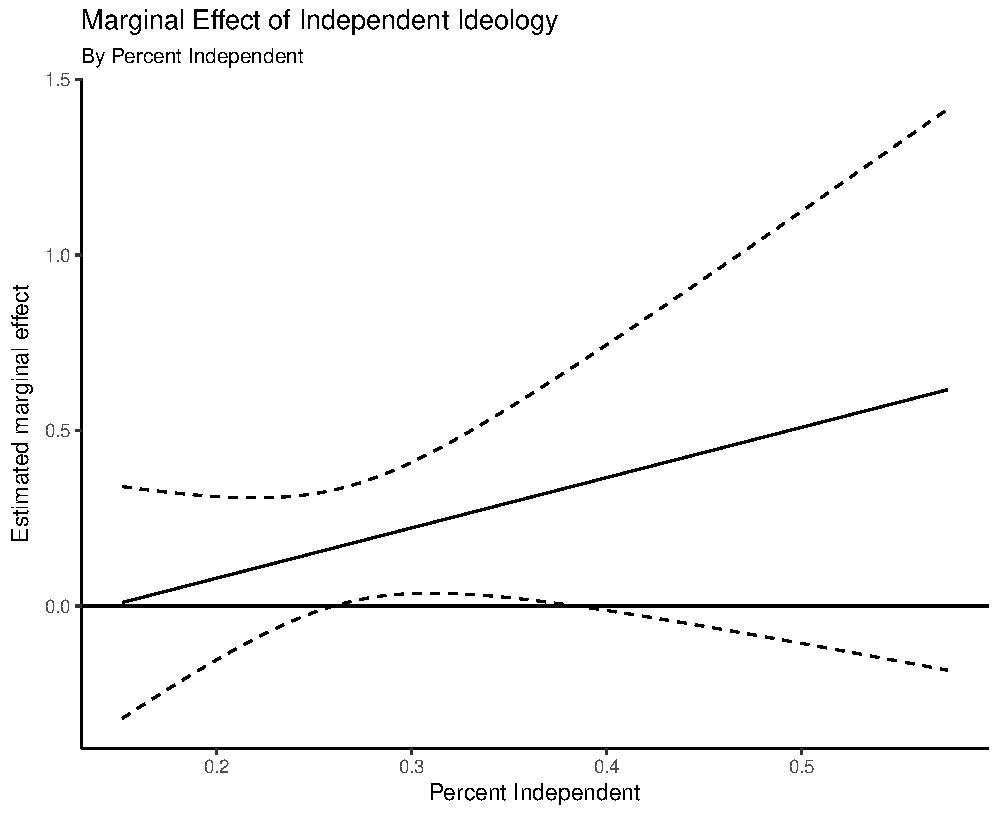
\includegraphics[width=.25\textwidth]{/Users/dsimp/GitHub/Clinton(2006)Rep/drafts/marginals/me3-4} &
    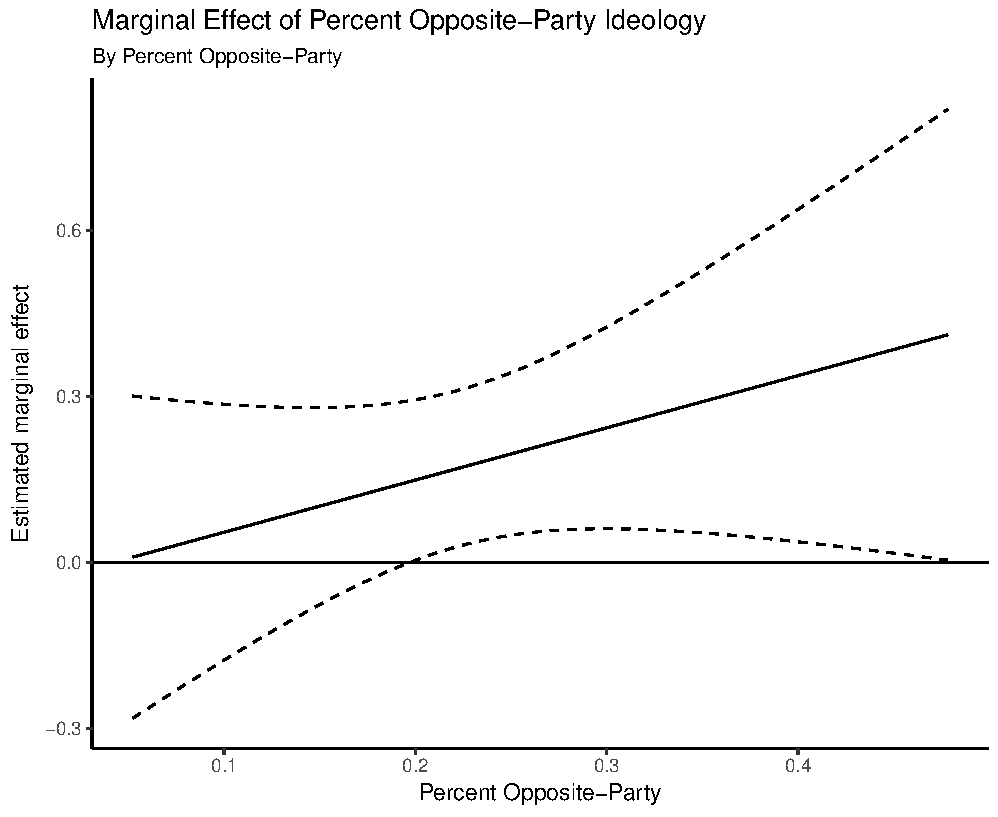
\includegraphics[width=.25\textwidth]{/Users/dsimp/GitHub/Clinton(2006)Rep/drafts/marginals/me3-6} \\
     & & \\
  \end{tabular}
    %}   
 \end{centering}\\
  \textbf{Note:} . 
\end{figure}
 

\newpage

\subsection{Signaled vs Revealed Responsiveness: Party Analysis with  Key Votes}

The previous section showed that across all votes legislators are responsive to their sub-district constituencies. Clinton (2006) argues that when ideal points are restricted to key votes the regression results show that the responsiveness puzzle is not sensitive to the stake of legislation considered (p. 405). However, Clinton's key vote analysis also omits the constitutive terms resulting in biased findings. Therefore, in this section I explore whether the above findings are consistent when the set of votes is restricted to key votes.

Author XXXX argued that a majority of House votes are insignificant. As such, it is my hypothesis that the all votes analysis displays greater conservative consistency than the key vote analysis. During the 106th House, the Republican Party controlled both houses of Congress, and the democratic party controlled the presidency. Under the Cartel Model \textbf{cite} it should be expected that the vast majority of bills that make it to the House floor for a vote are those that will gain a \textbf{blah.} Author xxx suggests that most of these bills are fluff. Such votes may be simple resolutions that have no policy consequence or those that have no chance of passing the Senate or overcoming a presidential veto. 

In the 106th House only XX bills were considered key legislation. Therefore, it is my expectation that the bills are largely used for Republican party to signal partisan loyalty. Democratic representatives may also use such bills to signal bipartisan credibility.

Since key legislation is likely to be politically salient and to make it to the president's desk, it is my hypothesis that the revealed responsiveness relationship will shows decreased responsiveness conservative ideology and increased responsiveness to liberal ideology for legislators of both parties. As such, the key legislation anlysis should reveal members of the Republican (Majority Party) to be less conservatively consistent on average and Democrats (the Minority Party) to be more liberally consistent.

I am still developing this signaled vs revealed responsiveness hypothesis. Should the findings align, it may only be correlative and coincidental. With one Congress's worth of data at this time, I am unable to distinguish between the effects of presidential power, party agenda control, district competitiveness, or other potential explanations. In future work, I plan to explore the data of more Congresses and to potentially develop a game theoretic model of signaled vs revealed responsiveness. The below results provide evidence that this line of research is worth further exploration.

\textbf{Results:} When the data is restricted to key votes, many of the previously observed responsiveness relationship change. Table 4 provides the key votes regression results and Figure 7 provides the key votes marginal effects plots. 

\textit{Same-party:} The first notable change is that the slops of the Republican same-party share and ideology plots are now negative. The all votes plots suggested that there may be a degree of increasing returns to ideology (share) for the relationship between legislator conservative ideological consistency and share (ideology) in panel (A) (panel (D)). However, the panel (A) key votes analysis potentially suggests decreasing returns to percent same party as previously found in the democratic ideology plot in panel (G).  The slope of the marginal effect lines in both (A) and (D) are also steeper in the key votes analysis. Panel (D) shows that party ideology is insignificant at all party sizes.

For Democrats, Panel (G) shows that relative to the all votes analysis, the key votes marginal effects plot shifted down and is more steep. The plot indicates increases consistency responsiveness to percent same party at all ideology levels. The plot again suggest decreasing returns to extremity. Similar to the Republican panel (D), Panel (J) same-party ideology is not significantly related to ideological consistency at any party size.

\textit{Opposite Party:} In the opposite party analysis, the Republican panel (C) shows a dramatically steeper marginal effects plot for opposite party share. In contrast, the Democratic panel (F) reveals no responsiveness to opposite party share.

\textit{Independents:} For Republicans, the independent plot looks very similar to the opposite party pots. For Democrats, the independent plots switch from a positive to negative slope, potentially showing a similar relationship to same party constituents, but with a larger magnitude of responsiveness.

\textbf{Summary:} Together, the plots show evidence that legislators display a different responsiveness relationship when the set of considered votes is restricted from all votes to key votes. Both parties display similar responsiveness to same-party constituents. The plots suggest legislators have a high degree of responsiveness to the ideology of their same party.



Figure X provides a spatial depiction of district group ideology and legislator ideal points.

Both panels contain a depiction of horizontal district bar graphs and legislator ideal points. Each horizontal bar is split into three sections, same-party share, independent share, and non-same party share. The shares are then filled by the their respective group ideology score, where liberal ideology is blue and conservative ideology is red. Districts are organized from top to bottom first by Democratic held districts in decreasing order of same party-share. Then by Republican held districts in increasing order of same party-share. As such the top horizontal bar in the plots represents the district with the largest share of identified Democrats. The bottom horizontal bar represents district with the largest share of identified Republicans. Districts in the center of the plot are those that have either same-party shares that are less than 50\% of the district XYZ.  

In the top panel a point is plotted for the relative legislator ideal point for each district. The points have been re-scaled to fit on a 0 to 1 scale.

The color represents.


 This can be see as the top horizontal bars are long blue  \textbf{blah.}







\newpage

\input{/Users/dsimp/GitHub/Clinton(2006)Rep/drafts/stargazer/table4.txt}


% Interaction Terms Key Votes
\begin{figure}[!htbp]
\caption{Marginal Effects of Interaction Terms (Key Votes)}
\begin{centering}
%\centering
%\fbox{
  \begin{tabular}{ccc}%{@{}ccc@{}}
	& \small \textbf{GOP Regression} & \\ 
	& & \\ 	
  	\small (A) Percent Same-Party& 
  	\small (B) Percent Independent& 
    \small (C) Percent Opposite-Party\\
    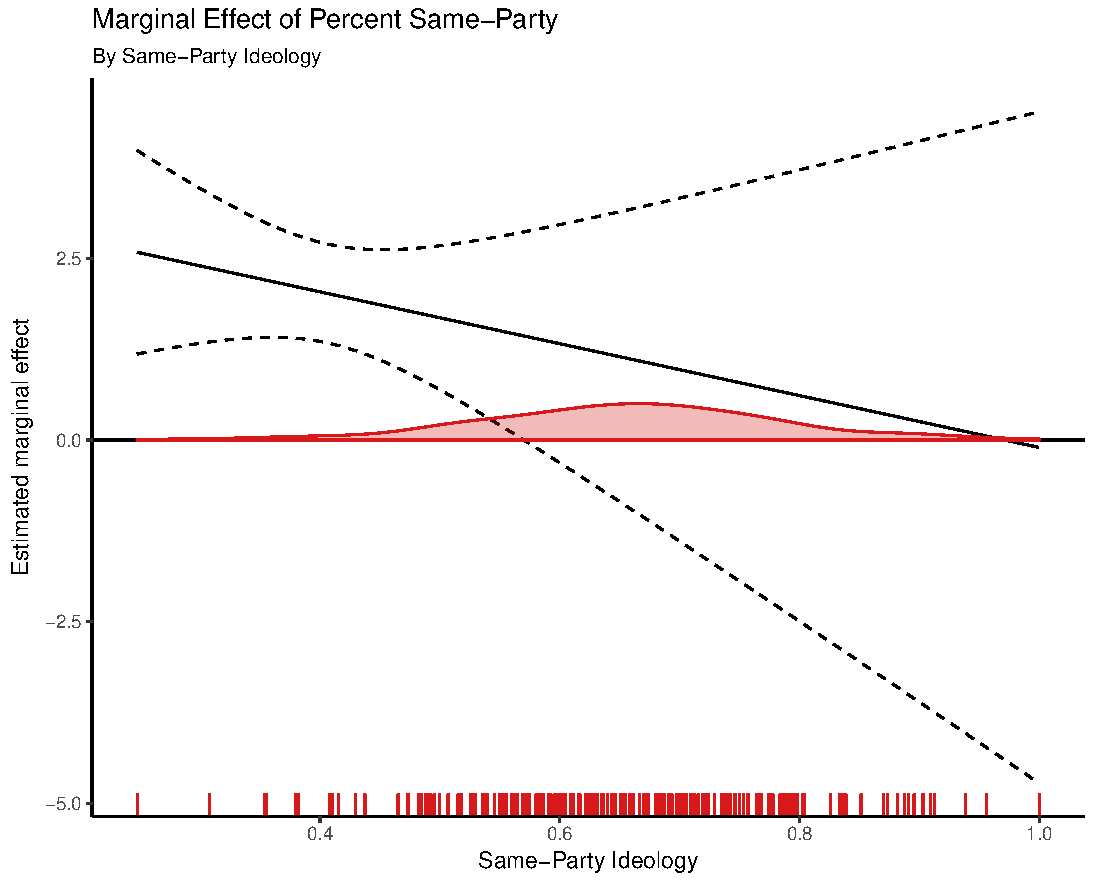
\includegraphics[width=.25\textwidth]{/Users/dsimp/GitHub/Clinton(2006)Rep/drafts/marginals/me4-1} &
    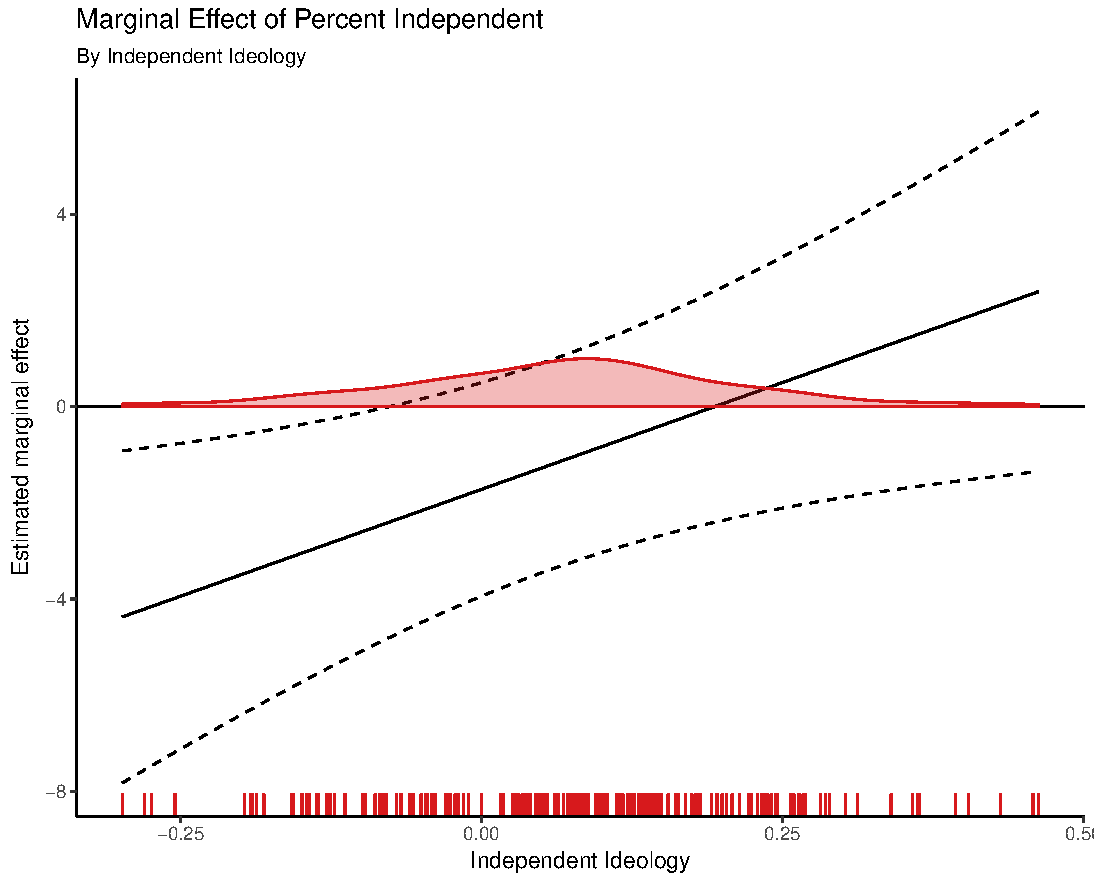
\includegraphics[width=.25\textwidth]{/Users/dsimp/GitHub/Clinton(2006)Rep/drafts/marginals/me4-3} &
    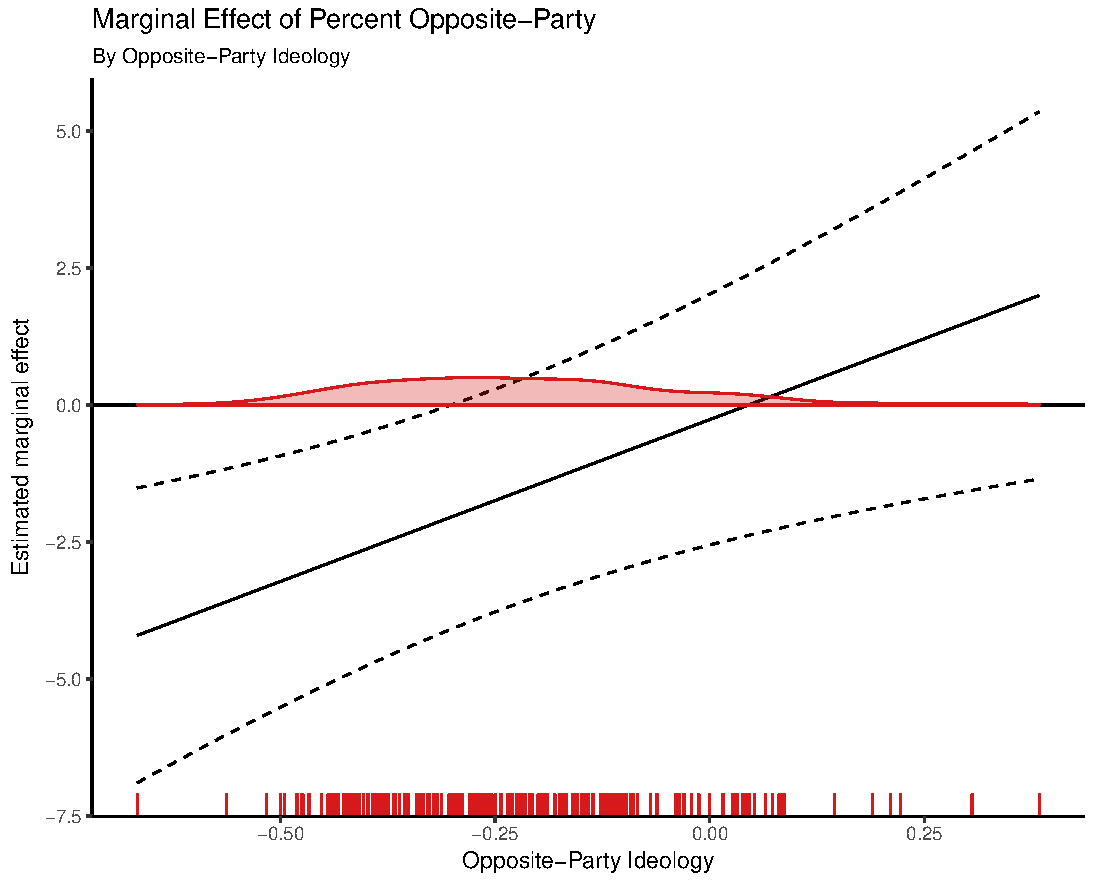
\includegraphics[width=.25\textwidth]{/Users/dsimp/GitHub/Clinton(2006)Rep/drafts/marginals/me4-5} \\
     & & \\
  	\small (D) Same-Party Ideology& 
  	\small (E) Independent Ideology& 
    \small (F) Opposite-Party Ideology\\
    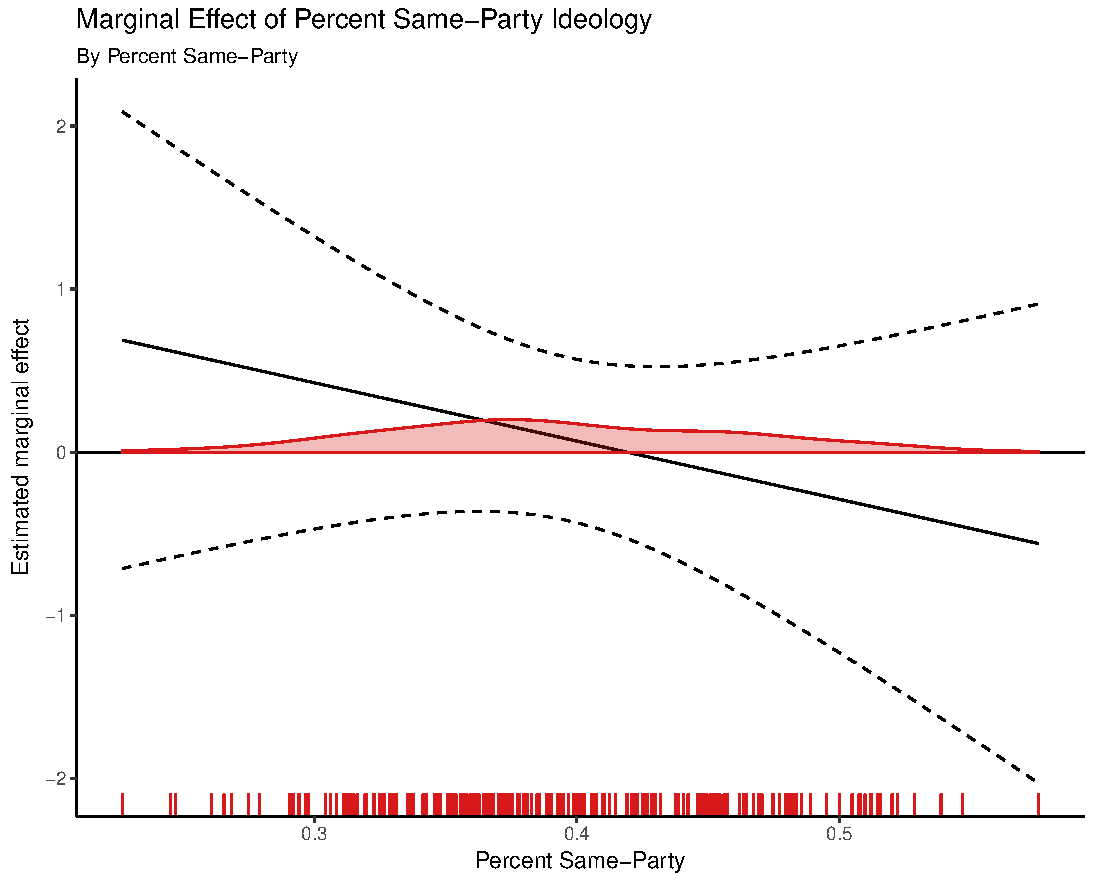
\includegraphics[width=.25\textwidth]{/Users/dsimp/GitHub/Clinton(2006)Rep/drafts/marginals/me4-2} &
    \includegraphics[width=.25\textwidth]{/Users/dsimp/GitHub/Clinton(2006)Rep/drafts/marginals/me4-4} &
    \includegraphics[width=.25\textwidth]{/Users/dsimp/GitHub/Clinton(2006)Rep/drafts/marginals/me4-6} \\
    	& & \\ 
	& \small \textbf{DEM Regression} & \\ 
	& & \\ 
  	\small (G) Percent Same-Party& 
  	\small (H) Percent Independent&  
    \small (I) Percent Opposite-Party\\
    \includegraphics[width=.25\textwidth]{/Users/dsimp/GitHub/Clinton(2006)Rep/drafts/marginals/me5-1} &
    \includegraphics[width=.25\textwidth]{/Users/dsimp/GitHub/Clinton(2006)Rep/drafts/marginals/me5-3} &
    \includegraphics[width=.25\textwidth]{/Users/dsimp/GitHub/Clinton(2006)Rep/drafts/marginals/me5-5} \\
     & & \\
  	\small (J) Same-Party Ideology& 
  	\small (K) Independent Ideology& 
    \small (H) Opposite-Party Ideology\\
    \includegraphics[width=.25\textwidth]{/Users/dsimp/GitHub/Clinton(2006)Rep/drafts/marginals/me5-2} &
    \includegraphics[width=.25\textwidth]{/Users/dsimp/GitHub/Clinton(2006)Rep/drafts/marginals/me5-4} &
    \includegraphics[width=.25\textwidth]{/Users/dsimp/GitHub/Clinton(2006)Rep/drafts/marginals/me5-6} \\
     & & \\
  \end{tabular}
    %}   
 \end{centering}\\
  \textbf{Note:} . 
\end{figure}
 

% 

\newpage
%\input{/Users/dsimp/GitHub/Clinton(2006)Rep/drafts/table3.txt}

\newpage


\newpage

\newpage


\section{Conclusion} 
This paper has demonstrated that independent voters cannot be lumped with opposite party voters when studying the relationship between legislator voting behavior and sub-district constituent ideology. It also explore the sensitivity of various forms of ideology measures.

Future extensions of this project include comparing the stability of the results with other measures of legislator ideal points as well as to employ MRP for individual topic analysis.

Possible extensions to this project include a more in depth analysis of the Non-Common scale issue. Potential datasets include DW-Nominate Scores as well as CF-Scores. Such analysis would further tease out the consistency of using legislator votes to measure the relationship between behavior and sub-district ideology.

Another extension could consider using survey data. I would plan to identify data relevant to key votes in the 106th House. I would then use MRP to consider the relationship between voter preferences and outcomes on kev votes by topic. This would allow me to compare legislator responsiveness to district ideology to legislator responsiveness to district issue preferences.


A longer term extension of this project would be to 

Election Results data to explore the behavior of legislators who won close elections.
Census data - to explore how legislator ideal points varies with district ideology and district demographic characteristics. 

\section{Next Steps} 

This section includes next steps and ideas for the next draft of this paper.

\textbf{Cosmetic Next Steps}
\begin{itemize}
\item Include an appendix table of the 106th House Key Votes.
\item Change the arrangement of the panels in Figure 3. Vertically align the marginal effects of party share and party ideology instead of vertically align.
\item Add a model 5 to Table 2 that includes all three groups (SP ,IND, and OP) in the regression.
\item Also, add an additional figure to demonstrate the marginal effects plots of the new model 5.
\end{itemize}

\textbf{Include}
\begin{itemize}
\item Include a model of three groups
\item \textit{Competitiveness:} I could explore whether the difference between signaled and revealed preference (all vs key vote difference) is correlated with the size of a legislators election victory. Though victory size is also likely endogenously related to district competitiveness.
\item \textit{Presidential Vote Share"} I could explore whether the 
all vs key vote difference is correlated districts with the percentage of Clinton voters in 1994 or Gore voters in 2000 
\end{itemize}

\textbf{Sensitivity Analysis}
\begin{itemize}
\item Explore the impact of different weight matrices. Clinton weights his standard errors using the number of constituent respondents in each district. As such, he excludes the total number of sampled individuals in the district. That is he does not count individuals who did not answer the ideology preference question. 
\item Include an appendix table of the 106th House Key Votes.
\end{itemize}

A second, those less problematic, issue in the \cite{Clinton2006} analysis is the blah. Often EIVreg is used when there is a low R-squared --> blah blah.

Clinton (2006) includes an errors in variable regression in the analysis following the practice of Gerald C. Wright, Robert S. Erikson and John P. McIver, and Fuller (1987).


\textbf{Non-Common Scale}

To consider the Non-Common Scales issue I propose running the equation (3) specification using two additional methods for generating ideology scores \textbf{DW-Nominate}, and \textbf{CF-Scores}. Though all three measures are correlated, this procedure will explore how different measures affect the slope between district opinion ideology and legislator ideal points. Furthermore, it will demonstrate why the Non-Common Scale problem implies that the slope and intercept of the responsiveness curve lack direct meanings.The representative ideal points in Clinton (2006) were generated using a methodology described in Clinton (2004).


I have reproduced Clinton (2009) Figure 1. Below it is followed by replication results from Clinton (2009) Table 1 and Table 2. In each table I have reproduced Clinton's OLS findings and also included replication regression where I use Same-Party Ideology, Independent Ideology and Opposite Party Ideology.



\newpage

\newpage

\bibliography{citations}

\newpage
\section{Appendix} 
% Reset & Rename the Name Configuration of Tables and Figures
\setcounter{table}{0}
\renewcommand{\thetable}{A\arabic{table}}
\setcounter{figure}{0}
\renewcommand{\thefigure}{A\arabic{figure}}

% Ideal Points Summary Table
%\input{/Users/dsimp/GitHub/Clinton(2006)Rep/drafts/summary/summary1.txt}
Table A1 provides the summary statistics for Welch's t-tests of Republican and Democratic legislator ideal points. The absolute ideal point is found by taking the absolute value of all ideal points.
\input{/Users/dsimp/GitHub/Clinton(2006)Rep/drafts/summary/summarystat1.txt} 

Table A2 provides summary statistics for district ideology and sub-district ideology and percent share of total constituents. The statistics are grouped by legislator party. For example, the mean ideology of Democratic constituents in an average district with a Republican legislator is -0.219. The corresponding mean share of the total Democratic voters in an average district with a Republican legislator is 33.3\%.
\input{/Users/dsimp/GitHub/Clinton(2006)Rep/drafts/summary/summary2.txt} 


% Figure A1 is histograms of Group shares.
\begin{figure}[!htbp]
\caption{Distribution of District Group Shares}
\begin{centering}
%\centering
%\fbox{
  \begin{tabular}{@{}cc@{}}
	% & & \\  	
  	\small (A) Same-Party Share &
    \small (B) Non-Same-Party Share  \\
    \includegraphics[width=.45\textwidth]{/Users/dsimp/GitHub/Clinton(2006)Rep/drafts/histogram/histogram2-1.pdf} &
    \includegraphics[width=.45\textwidth]{/Users/dsimp/GitHub/Clinton(2006)Rep/drafts/histogram/histogram2-2.pdf} \\
    % & & \\
    \small (C) Opposite-Party Share & 
    \small (D) Independent Share\\
    \includegraphics[width=.45\textwidth]{/Users/dsimp/GitHub/Clinton(2006)Rep/drafts/histogram/histogram2-3.pdf} &
    \includegraphics[width=.45\textwidth]{/Users/dsimp/GitHub/Clinton(2006)Rep/drafts/histogram/histogram2-4.pdf} \\
    % &  &\\
  \end{tabular}
    %}   
 \end{centering}
 \small~~~~~~~~\textbf{Note:} The histograms illustrate the distribution of constituency group share of total district voters. Districts are classified by the party of their legislator. The short dashed lines are the Republican controlled district means, the long dashed line are the Democratic controlled district means, and the dotted and dashed line is the chamber mean.
\end{figure}. 

% Figure A2 is Ideal Point and Group share plots.
\begin{figure}[!htbp]
\caption{Legislator Ideal Points and District Ideology Means}
\begin{centering}
%\centering
%\fbox{
  \begin{tabular}{@{}cc@{}}
	% & & \\  	
  	\small (A) Ideal Point &
    \small (B) Ideal Point  \\
    \small vs Same-Party Share & 
    \small vs Non-Same-Party Share\\
    \includegraphics[width=.45\textwidth]{/Users/dsimp/GitHub/Clinton(2006)Rep/drafts/plots/shareplot1.pdf} &
    \includegraphics[width=.45\textwidth]{/Users/dsimp/GitHub/Clinton(2006)Rep/drafts/plots/shareplot2.pdf} \\
    % & & \\
    \small (C) Ideal Point & 
    \small (D) Same-Party Ideology\\
    \small vs Opposite Party Share  & 
    \small vs Independent Share\\
    \includegraphics[width=.45\textwidth]{/Users/dsimp/GitHub/Clinton(2006)Rep/drafts/plots/shareplot3.pdf} &
    \includegraphics[width=.45\textwidth]{/Users/dsimp/GitHub/Clinton(2006)Rep/drafts/plots/shareplot4.pdf} \\
    % &  &\\
  \end{tabular}
    %}   
 \end{centering}
 \small~~~~~~~~\textbf{Note:} Districts represented by Republicans (Democrats) are plotted with triangles (circles). A bivariate trend line is plotted for overall comparison and party trend lines are plotted for comparison within districts.
\end{figure}. 

% Figure A3 is Key Ideal Point and Group share plots.
%\begin{figure}[!htbp]
\caption{Legislator Ideal Points and District Ideology Means}
\begin{centering}
%\centering
%\fbox{
  \begin{tabular}{@{}cc@{}}
	% & & \\  	
  	\small (A) Ideal Point &
    \small (B) Ideal Point  \\
    \small vs Same-Party Share & 
    \small vs Non-Same-Party Share\\
    \includegraphics[width=.45\textwidth]{/Users/dsimp/GitHub/Clinton(2006)Rep/drafts/plots/shareplot1.pdf} &
    \includegraphics[width=.45\textwidth]{/Users/dsimp/GitHub/Clinton(2006)Rep/drafts/plots/shareplot2.pdf} \\
    % & & \\
    \small (C) Ideal Point & 
    \small (D) Same-Party Ideology\\
    \small vs Opposite Party Share  & 
    \small vs Independent Share\\
    \includegraphics[width=.45\textwidth]{/Users/dsimp/GitHub/Clinton(2006)Rep/drafts/plots/shareplot3.pdf} &
    \includegraphics[width=.45\textwidth]{/Users/dsimp/GitHub/Clinton(2006)Rep/drafts/plots/shareplot4.pdf} \\
    % &  &\\
  \end{tabular}
    %}   
 \end{centering}
 \small~~~~~~~~\textbf{Note:} Districts represented by Republicans (Democrats) are plotted with triangles (circles). A bivariate trend line is plotted for overall comparison and party trend lines are plotted for comparison within districts.
\end{figure}. 


\input{/Users/dsimp/GitHub/Clinton(2006)Rep/drafts/stargazer/table2.2.txt}

\begin{figure}[!htbp]
\caption{Representative Ideal Points (Key Votes) and District Ideology (Three Groups)}
\begin{centering}
%\centering
%\fbox{
  \begin{tabular}{@{}cc@{}}
	 & \\  	
	\small (A) Marginal Effect of Percent Same-Party&	
  	\small (B) Marginal Effect of Same-Party Ideology\\
    \includegraphics[width=.45\textwidth]{/Users/dsimp/GitHub/Clinton(2006)Rep/drafts/marginals/mebk-1.pdf} &
    \includegraphics[width=.45\textwidth]{/Users/dsimp/GitHub/Clinton(2006)Rep/drafts/marginals/mebk-2.pdf} \\
     & \\
	\small (C) Marginal Effect of Percent Independent& 
    \small (D) Marginal Effect of Independent Ideology\\
    \includegraphics[width=.45\textwidth]{/Users/dsimp/GitHub/Clinton(2006)Rep/drafts/marginals/mebk-3.pdf} &
    \includegraphics[width=.45\textwidth]{/Users/dsimp/GitHub/Clinton(2006)Rep/drafts/marginals/mebk-4.pdf} \\
     &  \\
    \small (E) Marginal Effect of Percent Opposite-Party&  
    \small (F) Marginal Effect of Opposite-Party Ideology\\
    \includegraphics[width=.45\textwidth]{/Users/dsimp/GitHub/Clinton(2006)Rep/drafts/marginals/mebk-5.pdf} &
    \includegraphics[width=.45\textwidth]{/Users/dsimp/GitHub/Clinton(2006)Rep/drafts/marginals/mebk-6.pdf} \\
     &  \\
  \end{tabular}
    %}   
 \end{centering}
  \textbf{Note:} Each panel plots the respective marginal effect of the constitutive terms of the interaction variables in Table 2 Model 5.
\end{figure}
 

% Second Comparison Plot
\begin{figure}[!htbp]
\caption{District Group and Legislator Vote Distribution (Key Votes)}
\begin{centering}
%\centering
%\fbox{
  \begin{tabular}{c}%{@{}ccc@{}}
    \includegraphics[width=.80\textwidth]{/Users/dsimp/GitHub/Clinton(2006)Rep/drafts/compare/compare1b}\\
    \\
    \\
    \includegraphics[width=.80\textwidth]{/Users/dsimp/GitHub/Clinton(2006)Rep/drafts/compare/compare2}\\
    %\includegraphics[width=.25\textwidth]{/Users/dsimp/GitHub/Clinton(2006)Rep/drafts/marginals/me4-3}
  \end{tabular}
    %}   
 \end{centering}\\
 % \textbf{Note:} Words 
\end{figure}


% Data set summary table

\begin{sidewaystable}[!htbp] \centering 
  \caption{} 
  \label{} 
\begin{tabular}{@{\extracolsep{5pt}}lccccccc} 
\\[-1.8ex]\hline \\[-1.8ex] 
Statistic & \multicolumn{1}{c}{N} & \multicolumn{1}{c}{Mean} & \multicolumn{1}{c}{St. Dev.} & \multicolumn{1}{c}{Min} & \multicolumn{1}{c}{Pctl(25)} & \multicolumn{1}{c}{Pctl(75)} & \multicolumn{1}{c}{Max} \\ 
\hline \\[-1.8ex] 
Legislator Ideal Pt & 432 & 0.324 & 0.527 & $-$1.000 & $-$0.139 & 0.802 & 1.240 \\ 
Legisaltor Ideal Pt KV & 432 & 0.036 & 0.941 & $-$2.010 & $-$0.752 & 0.818 & 2.110 \\ 
Legislator Ideal Pt Prec & 432 & 45726.000 & 660212.000 & 98.300 & 519.000 & 933.000 & 9736997.000 \\ 
Legislator Ideal Pt KV Prec & 432 & 46029.000 & 675447.000 & 2.540 & 7.510 & 26.900 & 10074884.000 \\ 
District & 432 & 2797.000 & 1571.000 & 101 & 1304.0 & 4102.0 & 5600 \\ 
Party & 432 & 152.000 & 50.700 & 100 & 100 & 200 & 328 \\ 
Mean Ideolgoy & 432 & 0.126 & 0.172 & $-$0.618 & 0.034 & 0.253 & 0.526 \\ 
Mean SP Ideology & 432 & 0.211 & 0.487 & $-$0.858 & $-$0.257 & 0.661 & 1.000 \\ 
Mean NSP Ideology & 432 & 0.098 & 0.244 & $-$0.541 & $-$0.105 & 0.303 & 0.667 \\ 
Mean OP Ideology & 432 & 0.173 & 0.443 & $-$0.667 & $-$0.243 & 0.597 & 1.190 \\ 
Mean IND Ideology & 432 & 0.047 & 0.161 & $-$0.500 & $-$0.048 & 0.140 & 0.467 \\ 
StDev Ideology & 432 & 0.928 & 0.056 & 0.762 & 0.891 & 0.960 & 1.220 \\ 
StDev SP Ideology & 432 & 0.834 & 0.091 & 0.577 & 0.773 & 0.887 & 1.210 \\ 
StDev NSP Ideology & 432 & 0.879 & 0.080 & 0.681 & 0.823 & 0.923 & 1.330 \\ 
StDev OP Ideology & 432 & 0.843 & 0.115 & 0.515 & 0.775 & 0.903 & 1.550 \\ 
StDev IND Ideology & 432 & 0.852 & 0.104 & 0.577 & 0.786 & 0.910 & 1.280 \\ 
Respondents & 432 & 232.000 & 152.000 & 41 & 178 & 254 & 2099 \\ 
SP Respondents & 432 & 86.600 & 44.500 & 15 & 64 & 99.2 & 571 \\ 
NSP Respondents & 432 & 125.000 & 103.000 & 18 & 94 & 140 & 1443 \\ 
IND Respondents & 432 & 61.300 & 68.500 & 8 & 43 & 67 & 984 \\ 
OP Respondents & 432 & 64.100 & 39.500 & 6 & 45 & 76 & 459 \\ 
Avg 2P Pres Vote & 432 & 0.536 & 0.130 & 0.252 & 0.450 & 0.600 & 0.924 \\ 
District SqMi & 432 & 8.030 & 7.390 & $-$1 & 2 & 12 & 43 \\ 
Tenure & 432 & 8727.000 & 34470.000 & 0.000 & 421.000 & 7708.000 & 654334.000 \\ 
\hline \\[-1.8ex] 
\end{tabular} 
\end{sidewaystable} 









\end{document}